\documentclass{uai2026} % for initial submission
%\documentclass[accepted]{uai2026} % after acceptance, for a revised version

% If you set papersize explicitly, activate the following three lines:
%\special{papersize = 8.5in, 11in}
%\setlength{\pdfpageheight}{11in}
%\setlength{\pdfpagewidth}{8.5in}

%% Choose your variant of English; be consistent
\usepackage[american]{babel}

% If you use natbib package, activate the following three lines:
%\usepackage[round]{natbib}
%\renewcommand{\bibname}{References}
%\renewcommand{\bibsection}{\subsubsection*{\bibname}}
\usepackage{natbib}
% personal package including many pre-defined commands for convenience
%
% flush right qed marks, e.g. at end of proof
%
\usepackage[utf8]{inputenc} % allow utf-8 input
\usepackage[T1]{fontenc} 
\usepackage{graphicx}
\usepackage{subcaption}
\usepackage{lipsum}
\usepackage{amsfonts,nccmath,mathtools}
\usepackage{placeins}
\usepackage{amssymb}
\usepackage{epstopdf}
\usepackage{algorithm}
\usepackage{algpseudocode}
% Define Input/Output labels for algpseudocode:
\algnewcommand\algorithmicinput{\textbf{Input:}}
\algnewcommand\algorithmicoutput{\textbf{Output:}}
\algnewcommand\Input{\item[\algorithmicinput]}
\algnewcommand\Output{\item[\algorithmicoutput]}
\input{math_commands}
\input{defns}
\ifpdf
  \DeclareGraphicsExtensions{.eps,.pdf,.png,.jpg}
\else
  \DeclareGraphicsExtensions{.eps}
\fi
% \hypersetup{
%     colorlinks=true,
%     linkcolor=blue,
%     filecolor=magenta,      
%     urlcolor=cyan,
% }
% Add a serial/Oxford comma by default.
\newcommand{\creflastconjunction}{, and~}
% Used for creating new theorem and remark environments

% \newtheorem{assumption}{Assumption}
% \newtheorem{hypothesis}{Hypothesis}
% \newtheorem{proof_sketch}{Sketch of proof}
% \newtheorem{myclaim}{Claim}
% \newtheorem{remark}{Remark}
% \newtheorem{mydef}{Definition}
% \newtheorem{prop}{Proposition}
% \newtheorem{mypro}{Property}
% Sets running headers as well as PDF title and authors
%\headers{}{D. Doe, P. T. Frank, and J. E. Smith}

% Title. If the supplement option is on, then "Supplementary Material"
% is automatically inserted before the title.
\usepackage{amsopn}
%\DeclareMathOperator{\diag}{diag}
% \usepackage{ulem}
\usepackage{xcolor}
\usepackage{amsthm}
\usepackage{booktabs}   % for \toprule, \midrule, \bottomrule
\usepackage{adjustbox}  % for \begin{adjustbox}{max width=\linewidth}

\newcommand{\blue}[1]{\textcolor{blue}{#1}}

\usepackage{enumitem}
\newcommand{\PLcirc}{\texttt{P\L$^\circ$}}
\usepackage{indentfirst}
\usepackage{bm}
\usepackage{kantlipsum}
%\usepackage{showframe}
\allowdisplaybreaks
\usepackage{adjustbox}
\usepackage{cleveref}
% Avoid duplicate hyperref anchors for algorithmic line numbers across multiple algorithms.
\makeatletter
\renewcommand{\theHALG@line}{ALG@line.\thealgorithm.\arabic{ALG@line}}
\makeatother
% \usepackage{titlesec}
% \titlespacing*{\section}{0pt}{0.1\baselineskip}{0.2\baselineskip}
% \usepackage{titlesec}
% \titlespacing*{\section}{0pt}{0.1\baselineskip}{0.2\baselineskip}
% \DeclareMathOperator{\Tr}{\text{\rm{Tr}}}
% \DeclareMathOperator*{\argmax}{arg\,max}
% \DeclareMathOperator*{\argmin}{arg\,min}


\let\Tr\relax
\let\argmax\relax
\let\argmin\relax
\let\ceil\relax
\let\floor\relax
\let\eg\relax
\let\ie\relax

% Standard optimization operators (avoid conflicts with imported macros above).
\DeclareMathOperator*{\argmin}{arg\,min}
\DeclareMathOperator*{\argmax}{arg\,max}

\newtheorem{thm2}{Theorem [informal]}
\newtheorem{theorem}{Theorem}[section]
\newtheorem{lemma}{Lemma}[section]
\newtheorem{prop}{Proposition}[section]
\newtheorem{remark}{Remark}[section]
\newtheorem{corollary}{Corollary}[section]
\newtheorem{mydef}{Definition}[section]
\newtheorem{assumption}{Assumption}
%\newtheorem{lemma}{Lemma}
\newtheorem{result}{Result}
\newtheorem{step}{Step}
\counterwithin*{step}{section}

%\newtheorem{proposition}{Proposition}
%\newtheorem{corollary}{Corollary}
%\newtheorem{conjecture}{Conjecture}
%\newtheorem{definition}{Definition}
%\newtheorem{remark}{Remark}
\newtheorem{example}{Example}
%\newtheorem{question}{Question}
% \newtheorem*{theorem}{Theorem}
\newtheorem{desiderata}{Desiderata}
\newtheorem{desideratum}{Desideratum}
% \crefalias{desiderata}{desiderata}
% \crefalias{desideratum}{desideratum}
\crefname{desideratum}{desideratum}{desiderata}
\crefname{result}{result}{results}
\crefname{step}{step}{steps}
\Crefname{step}{Step}{Steps}
\crefname{assumption}{assumption}{assumptions}
\crefname{lemma}{lemma}{lemmas}
\Crefname{lemma}{Lemma}{Lemmas}

\newcommand{\norm}[1]{\left\lVert #1 \right\rVert}
\newcommand{\inner}[2]{\left\langle #1,#2 \right\rangle}
\newcommand{\EE}{\mathbb{E}}
\newcommand{\F}{\mathcal{F}}
\newcommand{\Reg}{\mathsf{Reg}}

\title{Online Bilevel Optimization without Hyper-Gradients: Fully First-Order Single-Loop Methods}
\author{Anonymous Author(s)}
% If you use BibTeX in apalike style, activate the following line:
%\bibliographystyle{apalike}

\begin{document}
\onecolumn
\maketitle

% If your paper is accepted and the title of your paper is very long,
% the style will print as headings an error message. Use the following
% command to supply a shorter title of your paper so that it can be
% used as headings.
%
%\runningtitle{I use this title instead because the last one was very long}

% If your paper is accepted and the number of authors is large, the
% style will print as headings an error message. Use the following
% command to supply a shorter version of the authors names so that
% they can be used as headings (for example, use only the surnames)
%
%\runningauthor{Surname 1, Surname 2, Surname 3, ...., Surname n}

\begin{abstract}
We study online bilevel optimization (OBO), where at each round the upper-level objective is evaluated at the follower’s implicit solution of a time-varying lower-level problem. We propose \emph{VR--SF$^2$OBO}, a variance-reduced, fully first-order, single-loop algorithm that avoids linear-system solves and Hessian--vector products. Under a strongly convex lower level, we establish a sublinear \emph{stochastic bilevel local-regret} bound that scales with the upper-level value drift, the follower path length, and gradient drift; no additional Hessian/Jacobian variation budgets appear in the final rate, and the bound recovers offline rates when drift vanishes. This contrasts with online hyper-gradient methods, which obtain sharper horizon dependence at the cost of stronger second-order oracles. Empirically, on online loss tuning for imbalanced data and meta-learning under distribution shift, our methods achieve accuracy comparable to hyper-gradient baselines while offering the lower per-round runtime than alternating-gradient and window-smoothed OBO competitors.
% We study online bilevel optimization (OBO), where each round evaluates an upper objective at the follower’s implicit solution of a time-varying lower-level problem. We introduce F$^2$OBO, a fully first-order, single-loop, window-free method that avoids linear-system solves and Hessian–vector products, and we develop VR–SF$^2$OBO, a variance-reduced stochastic variant. Under the standard lower-level strong-convexity, our analysis yields bilevel local-regret bounds that scale with natural variation budgets—upper-objective value drift and the follower path-length and recover offline rates when drift vanishes. In the stochastic case, our local-regret is sublinear and depends only on gradient-drift and path-length terms; with a constant penalty parameter, no additional Hessian/Jacobian variation budgets appear in the final rate, highlighting a contrast with online hyper-gradient approaches that achieve sharper horizon dependence but rely on stronger second-order oracles. Empirically, on online loss tuning for imbalanced data and meta-learning under distribution shift, our methods obtains the comparable accuracy to the hyper-gradient methods while delivering significantly lower per-round runtime than alternating-gradient and window-smoothed OBO baselines.
% We study \emph{online bilevel optimization} (OBO), where at each round a time-varying lower-level problem is (approximately) solved and the upper-level objective is evaluated at the lower-level implicit solution. We introduce \emph{F$^2$OBO}, a fully first-order, \emph{single-loop} method that avoids linear-system solves, Hessian--vector products, and window smoothing. Under a lower-level strongly-convexity assumption, we establish \emph{bilevel local-regret} bounds that scale with natural \emph{variation budgets}—capturing upper-level objective drift and the follower's optimal path length—and recover static rates when drift vanishes. We further propose \emph{VR--SF$^2$OBO}, a variance-reduced stochastic variant that achieves sublinear local regret using $\mathcal{O}(1)$ batch sizes while preserving the same single-loop update. Empirically, on online loss tuning and meta-learning under distribution shift, our methods match or improve accuracy while delivering significantly lower per-round runtime than alternating-gradient and window-smoothed OBO baselines.
\end{abstract}

\section{Introduction}\label{sec:intro}
Bilevel optimization (BO) aims to minimize an \emph{upper-level} objective that is evaluated at the solution of a \emph{lower-level} optimization problem. Originating in game theory \citep{von1953theory} and later formalized within mathematical optimization \citep{bracken1973mathematical}, BO underpins a range of modern machine learning workflows: hyperparameter optimization and implicit differentiation \citep{lorraine2020implicit,franceschi2018bilevel}, meta-learning \citep{ji2021bilevel}, reinforcement learning \citep{stadie2020intrinsic}, and neural architecture search as well as loss-shaping pipelines \citep{liu2018darts,li2021autobalance} all admit natural bilevel formulations.
Classical theory largely consider the \emph{offline} regime—objectives are fixed and the goal is to find a single stationary point (or minimizer) \citep{bracken1973mathematical,maclaurin2015reversible,ji2021bilevel,chen2025fullyfirstorder}. By contrast, many real-world systems are inherently \emph{online}: inputs and labels drift over time \citep{gama2014conceptdrift,quionero2009datasetshift}, objectives evolve under variation budgets in online optimization \citep{besbes2015nonstationary}, reward structures change in nonstationary RL \citep{padakandla2019nonstationary}, and resource-aware deployments face hardware-dependent latency/energy constraints \citep{cai2020onceforall}. In these settings, the learner must update decisions on the fly from partial, noisy feedback, rather than repeatedly solving a fixed bilevel problem.\\
Online bilevel optimization (OBO) captures dynamic settings where objectives change over time, requiring the leader to continuously adjust the upper-level decision in response to the follower’s (implicit) solution. As in online single-level optimization \citep{hazan2016oco}, OBO proceeds via iterative decisions made without advance knowledge of outcomes \citep{tarzanagh2024online,OBORegretAnon}. We define online bilevel optimization (OBO) at round \(t\) by
\begin{align}\label{eq_def_OBO}
\min_{x \in \mathbb{R}^{d_1}} \;\; \phi_t(x) &:= f_t\bigl(x, y_t^{*}(x)\bigr) \\
\text{s.t.}\quad y_t^{*}(x) &= \arg\min_{y \in \mathbb{R}^{d_2}} g_t(x,y).
\end{align}
Here, \(x\) and \(y\) are the upper- and lower-level variables, and \(f_t\) and \(g_t\) are the corresponding time-varying objectives for \(t \in \{1,\dots,T\}\).
Over \(T\) rounds, the leader selects \(x_t \in \mathbb{R}^{d_1}\) without knowing \(y_t^{*}(x_t)\); instead, it uses a follower-provided estimate \(y_t\) based on limited information about \(g_t\), and incurs the outer loss \(f_t(x_t, y_t)\).


This setting extends online single-level optimization to \emph{nested} objectives and is correspondingly more challenging: to optimize
\(\phi_t(x)\),
the leader only has access to an approximate follower state \(y_t\) and the history of past objectives \(\{(f_k,g_k)\}_{k\le t-1}\).
Leveraging this history can improve the tracking of the solution map $y^{*}_{t}(x)$ and thus refine \(y_t\) as its estimate,
but residual tracking error $\|y_{t}-y^{*}_{t}(x_{t})\|$ and temporal drift of $(f_{t},g_{t})$ directly impact outer-level performance.
Recent OBO methods typically alternate lower- and upper-level updates and evaluate performance via dynamic regret against a time-varying comparator. However, many of these approaches either assume strong oracle access—e.g., exact linear-system solves to compute hyper-gradients—or adopt \emph{window-smoothed} (sliding-window) regret definitions that improve stability but dull responsiveness to rapid changes \citep{tarzanagh2024online,lin2024nonconvex}.

\paragraph{Challenges.}
OBO inherits the difficulties of online nonconvex learning and compounds them with the nested structure of BO: the \emph{hyper-gradient} $\nabla\phi_t$ depends simultaneously on (i) the current follower solution $y_t^{*}(x)$ and (ii) second-order information of the follower objective $g_t$. Classic hyper-gradient estimators either use implicit differentiation with linear-system solves/Hessian–vector products \citep{pedregosa2016hyperparameter,gould2016argmin,lorraine2020implicit} or differentiate through unrolled inner iterations \citep{maclaurin2015reversible,franceschi2017forwardreverse,franceschi2018bilevel}. In online settings, methods such as OAGD and SOBOW add history/window smoothing and often perform multiple inner iterations per round to temper drift and variance \citep{ataee2024oagd,lin2023sobow,bohne2024sobbo}, which may not accurately reflect system performance when functions change rapidly. In contrast, the SOGD approach \citep{anonymous2025stochastic} reduces oracle requirements for hyper-gradient estimation and achieves sublinear regret \emph{without} window smoothing.
We propose \textbf{F$^2$OBO}, a \emph{fully first-order, single-loop} OBO method that avoids Hessian–vector products and linear-system solves, together with its stochastic variance-reduced variant \textbf{VR--SF$^2$OBO}. Both algorithms adopt a penalty-based outer objective and take first-order outer steps using the same class of fully first-order hyper-gradient directions developed for offline BO \citep{chen2025fullyfirstorder,kwon2023fully,ChenMaZhang2025}. Analytically, we establish sublinear deterministic and stochastic \emph{bilevel local regret} bounds for F$^2$OBO and VR--SF$^2$OBO, respectively.
% Each round require $\mathcal{O}(1)$ per-round gradient evaluations tailored to time-varying environments.
\paragraph{Contributions.}
\begin{itemize}
\item \textbf{Fully first-order, single-loop OBO.} We propose \textbf{F$^2$OBO}, which performs one penalized inner step, one tracker step, and one outer update per round using only gradients of $(f_t,g_t)$—no Hessian--vector products and no linear-system solves.
\item \textbf{Deterministic local-regret with variation budgets.} Under standard assumptions (lower-level strong convexity; smoothness), we prove an average gradient local-regret bound that scales with outer value-variation and follower path-length, recovering the static scaling of batch bilevel methods when drift vanishes \citep{ji2021bilevel,chen2025fullyfirstorder}.
\item \textbf{Stochastic variance reduction.} We propose \textbf{VR--SF$^2$OBO}, a STORM-style variance-reduced variant with $\mathcal{O}(1)$-sized mini-batches, and establish a stochastic bilevel local-regret bound under standard oracle models.
\item \textbf{Experiment results.} Compared to OAGD/SOBOW/OBBO, our methods avoid window smoothing and multi-iteration inner solves \citep{ataee2024oagd,lin2023sobow,bohne2024sobbo}, improving responsiveness and per-round efficiency in nonstationary regimes.
\end{itemize}

\subsection*{Related Work}

\textbf{Foundations and offline bilevel optimization.}
Comprehensive treatments of BO and its links to MPECs appear in \citet{dempe2002foundations,colson2007overview}. 
Two dominant offline paradigms are implicit differentiation (ID/AID) \citep{pedregosa2016hyperparameter,gould2016argmin,lorraine2020implicit} and iterative/unrolled differentiation (ITD) \citep{maclaurin2015reversible,franceschi2017forwardreverse,franceschi2018bilevel}. 
Recent analyses provide convergence for nonconvex--strongly-convex bilevel problems and show that \emph{fully first-order} algorithms can attain near-optimal complexity without Hessian-vector products \citep{ji2021bilevel,chen2025fullyfirstorder}. 
Variance-reduced bilevel frameworks and estimators have also been developed \citep{dagreou2022framework,fang2018spider,cutkosky2019storm}.

\textbf{Online bilevel optimization (OBO).}
OAGD introduces dynamic/static bilevel regret and path-length measures for both inner and outer minimizers \citep{ataee2024oagd}. 
SOBOW proposes a single-loop, \emph{window-averaged} hyper-gradient method that achieves sublinear bilevel local regret without requiring access to past objectives \citep{lin2023sobow}, and subsequent work extends to Bregman geometries and stochastic variants with window averaging (OBBO/SOBBO) \citep{bohne2024sobbo}. 
Our approach differs by (i) keeping one update per level without window smoothing, and (ii) adopting proxy-based outer steps with fully first-order directions \citep{chen2025fullyfirstorder}.

\textbf{Online nonconvex learning and local regret.}
Because external regret is typically unattainable for general nonconvex losses, online analyses focus on gradient/prox-gradient stationarity notions \citep{hallak2021prox,heliou2020imperfect,heliou2021zeroth}; we follow this line for OBO and use standard OCO tools for context \citep{hazan2016oco}.


\section{Problem Setup and Notation}
\label{sec:setup}

We consider an online bilevel problem over rounds $t=1,\ldots,T$. At each round $t$, we are given differentiable functions
\[
f_t,g_t:\R^{d_1}\times\R^{d_2}\to\R.
\]
For a leader decision $x\in\R^{d_1}$, the follower solves
\[
y_t^{*}(x)\in\argmin_{y\in\R^{d_2}} g_t(x,y),
\]
and the (time-varying) \emph{hyper-objective} is
\[
\phi_t(x)\;:=\; f_t\!\big(x,\,y_t^{*}(x)\big).
\]
We focus on the unconstrained leader case $X=\R^{d_1}$.\footnote{The constrained case can be handled by replacing the outer update with a projection onto $X$; we omit these standard details.} In this setting, the gradient local regret is defined as follows:
\begin{equation}
\label{eq:local-regret}
\Reg^{\text{loc}}_T\;:=\;\frac1T\sum_{t=1}^T \big\|\nabla \phi_t(x_t)\big\|^2.
\end{equation}

\paragraph{Penalized proxy and notation.}
For a penalty parameter $\lambda>0$, define the penalized lower-level objective and its value function
\begin{align}
L_{\lambda,t}(x,y)&:= f_t(x,y)+\lambda\Big(g_t(x,y)-\min_{z} g_t(x,z)\Big),\\
L^{*}_{\lambda,t}(x)&:= \min_{y} L_{\lambda,t}(x,y),
\end{align}
and denote by $y^{*}_{\lambda,t}(x)\in\argmin_{y}L_{\lambda,t}(x,y)$ a (measurable) minimizer.
Note that for each fixed $x$, the term $\min_z g_t(x,z)$ is constant in $y$, so $y^{*}_{\lambda,t}(x)$ is equivalently defined by
$y^{*}_{\lambda,t}(x)\in\arg\min_y \bigl(f_t(x,y)+\lambda g_t(x,y)\bigr)$.
We will use the shorthands
\[
\ell\;:=\;\max\{C_f,\,L_f,\,L_g,\,\rho_g\},\qquad \kappa\;:=\;\ell/\mu.
\]

\begin{assumption}[Uniform regularity across $t$]\label{ass:offline}
Uniformly for all rounds $t$ and all $(x,y)$:
\begin{enumerate}
\item[\textnormal{(A1)}] \textbf{Lower level strong convexity.} $g_t(x,\cdot)$ is $\mu$–strongly convex: $\nabla^2_{yy} g_t(x,y)\succeq \mu I$.
\item[\textnormal{(A2)}] \textbf{First–order smoothness.} $\nabla f_t$ and $\nabla g_t$ are $L_f$– and $L_g$–Lipschitz in $(x,y)$, respectively.
\item[\textnormal{(A3)}] \textbf{Second–order regularity (in $y$).} $\nabla^2 g_t$ is $\rho_g$–Lipschitz in $y$: 
$\|\nabla^2 g_t(x,y)-\nabla^2 g_t(x,y')\|\le \rho_g\|y-y'\|$.
\item[\textnormal{(A4)}] \textbf{Follower Lipschitz in value.} $f_t(x,\cdot)$ is $C_f$–Lipschitz in $y$:
$|f_t(x,y)-f_t(x,y')|\le C_f\|y-y'\|$.
\end{enumerate}
Let $\ell:=\max\{C_f,L_f,L_g,\rho_g\}$ and $\kappa:=\ell/\mu$.
% \emph{Consequences used throughout:} (i) $y_t^{*}(x)$ and $y^{*}_{\lambda,t}(x)$ are single–valued and Lipschitz in $x$ with moduli $L_g/\mu$ and $4L_g/\mu$; 
% (ii) for $\lambda\ge 2L_f/\mu$, $\nabla L^{*}_{\lambda,t}$ is $L$–Lipschitz in $x$ with $L=O(\ell\kappa^3)$, and
% $\|\nabla L^{*}_{\lambda,t}(x)-\nabla\phi_t(x)\|\le D_1/\lambda$ for $\phi_t(x):=f_t(x,y_t^{*}(x))$ and $D_1=O(\ell\kappa^3)$. 
\end{assumption}

\paragraph{Variation budgets.}
Our analysis measures nonstationarity via the upper-level objective drifts and the path-length budgets:
\begin{align}
V_{T}^{f}\;&:=\;\sum_{t=2}^T\;\sup_{x,y}\;\big|\,f_{t}(x,y)-f_{t-1}(x,y)\,\big|,\label{eq_hyp_obj_seq_len}\\
H_{1,T}\;&:=\;\sum_{t=2}^T\;\sup_{x}\;\big\|\,y_t^{*}(x)-y_{t-1}^{*}(x)\,\big\|.\label{eq_path_len_1}\\
H_{2,T}\;&:=\;\sum_{t=2}^T\;\sup_{x}\;\big\|\,y_t^{*}(x)-y_{t-1}^{*}(x)\,\big\|^2.\label{eq_path_len}
\end{align}
% These budgets will appear in our regret bounds together with the proxy–hyper closeness terms that decay as $O(\lambda^{-2})$.

\section{Algorithm: F$^2$OBO (Window-Free)}
\label{sec:algo-window-free}

\paragraph{Variation budgets.}
Let $\{\phi_t\}_{t=1}^T$ denote the time-varying hyper-objectives
$\phi_t(x) := f_t(x, y_t^\star(x))$ where $y_t^\star(x)\in\arg\min_y g_t(x,y)$.
We quantify nonstationarity via two standard budgets in \eqref{eq_hyp_obj_seq_len} and \eqref{eq_path_len_1}.

\paragraph{Performance metric (window-free local regret).}
\[
\mathsf{Reg}^{\mathrm{loc}}_{T}
\;:=\;
\frac{1}{T}\sum_{t=1}^{T}\bigl\|\nabla\phi_t(x_t)\bigr\|^2.
\]

% ========================= Algorithm (outer unwindowed, inner per-round) =========================
\begin{algorithm}[H]
\caption{F$^2$OBO (outer \emph{unwindowed}; inner per-round)}
\label{alg:f2obo-perround-inner-windowfree}
\begin{algorithmic}[1]
\State \textbf{Inputs:} penalty $\lambda\ge 2L_f/\mu$; stepsizes $\{\eta^x_t,\eta^y_t,\eta^z_t\}$.
Initialize $(x_0,y_0,z_0)$.
\For{$t=0,\dots,T-1$}
\State \textbf{Inner (penalized, per-round):}\quad $y_{t+1}=y_t-\eta^y_t\big(\nabla_y f_t(x_t,y_t)+\lambda\,\nabla_y g_t(x_t,y_t)\big)$
\State \textbf{Inner (unpenalized, per-round):}\quad $z_{t+1}=z_t-\eta^z_t\,\nabla_y g_t(x_t,z_t)$
\State \textbf{Outer (unwindowed):}\quad
$x_{t+1}=x_t-\eta^x_t\Big(\nabla_x f_t(x_t,y_t)+\lambda\big(\nabla_x g_t(x_t,y_t)-\nabla_x g_t(x_t,z_t)\big)\Big)$
\EndFor
\end{algorithmic}
\end{algorithm}

This is the single-step, time-varying specialization of F2BA; it uses the same fully first-order search direction as in Eq.~(6) of \citet{ChenMaZhang2025}.

\section{Analysis under Bounded Variation Budgets (Window-Free)}
\label{sec:windowfree-analysis}

\paragraph{Assumptions.}
We work under Assumption~\ref{ass:offline}. Let $L_\phi$ be a uniform smoothness constant of $\{\phi_t\}_{t=1}^T$
(see Lemma~\ref{lem:descent_phi}).
We assume bounded variation budgets $V_T^f<\infty$, $H_{1,T}<\infty$, and $H_{2,T}<\infty$.
We further take $\lambda\ge 2L_f/\mu$ and stepsizes satisfying, for all $t$,
\[
\eta_t^x\le \frac{1}{2L_\phi},\qquad
\eta_t^y\le \frac{1}{L_f+\lambda L_g},\qquad
\eta_t^z\le \frac{1}{L_g}.
\]

\begin{theorem}[Window-free local regret with bounded variation]
\label{thm:windowfree}
Under the conditions above, Algorithm~\ref{alg:f2obo-perround-inner-windowfree} yields
\[
\frac{1}{T}\sum_{t=1}^T \|\nabla\phi_t(x_t)\|^2
\;\;\le\;\;
\tilde O\!\Big(\frac{1}{\sqrt{T}}\Big)
\;+\;\tilde O\!\Big(\frac{V_T^f + H_{1,T}+ H_{2,T}}{\sqrt{T}}\Big)
\;+\;O\!\Big(\frac{1}{\lambda^2}\Big)
\;+\;O\!\Big(\frac{\|y_0-y^{*}_{\lambda,1}(x_0)\|^2+\|z_0-y^{*}_{1}(x_0)\|^2}{T}\Big).
\]
In particular, if $V_T^f=o(\sqrt{T})$ and $H_{1,T}+H_{2,T}=o(\sqrt{T})$, then $\mathsf{Reg}^{\mathrm{loc}}_{T}=o(1)$ as $T\to\infty$
(e.g., by taking $\lambda=\lambda_T\to\infty$ so that the $O(1/\lambda^2)$ bias vanishes).
\end{theorem}

\begin{proof}[Proof sketch]
(i) \emph{Proxy gradient accuracy.} By Lemma~\ref{lem:offline-keys} (proxy vs.\ true hyper-gradient),
$\|\nabla L^{*}_{\lambda,t}(x_t)-\nabla\phi_t(x_t)\|\le D_1/\lambda$.
Moreover, by Lipschitzness of $\nabla_x f_t,\nabla_x g_t$ in $y$ (Assumption~\ref{ass:offline}),
the algorithmic direction
\[
d_t:=\nabla_x f_t(x_t,y_t)+\lambda\big(\nabla_x g_t(x_t,y_t)-\nabla_x g_t(x_t,z_t)\big)
\]
approximates $\nabla L^{*}_{\lambda,t}(x_t)$ up to the inner tracking errors
$e_t^y:=\|y_t-y^{*}_{\lambda,t}(x_t)\|$ and $e_t^z:=\|z_t-y_t^{*}(x_t)\|$.

(ii) \emph{Single-step descent.} Lemma~\ref{lem:descent_phi} bounds one outer step
$\phi_t(x_{t+1})-\phi_t(x_t)$ by (a) a descent term $-\eta_t^x\|\nabla\phi_t(x_t)\|^2$,
(b) a proxy bias term $O(\eta_t^x/\lambda^2)$, and (c) inner tracking terms proportional to
$\eta_t^x (e_t^y)^2$ and $\eta_t^x (e_t^z)^2$.

(iii) \emph{Tracking error of inner iterates.} One penalized and one unpenalized step ensure
$\|y_{t+1}-y_{\lambda,t}^{*}(x_t)\|^2$ and $\|z_{t+1}-y_t^{*}(x_t)\|^2$ contract up to the movement of
$y_{\lambda,t}^{*}$ and $y_t^{*}$ and the outer motion of $x_t$; see Lemma~\ref{lem:tracking}.
Summing the resulting recursion yields an $O(H_{2,T})$ contribution (plus initialization terms),
and allows absorption of the $\sum_t \eta_t^x (e_t^y)^2$ and $\sum_t \eta_t^x (e_t^z)^2$ terms appearing in (ii).

(iv) \emph{Nonstationarity control.} The change of objective across rounds contributes
$\sum_{t=2}^T \bigl(\phi_t(x_t)-\phi_{t-1}(x_t)\bigr)$.
By adding and subtracting $f_{t-1}(x_t,y_t^*(x_t))$ and using the $C_f$-Lipschitzness of $f_t(x,\cdot)$,
this term is controlled by $V_T^f+ C_f H_{1,T}$.

Choosing $\eta_t^x=\eta_x=\Theta(T^{-1/2})$ and combining (i)–(iv) yields the bound, together with the
$O(1/\lambda^2)$ proxy bias and $O(1/T)$ initialization terms.

\smallskip
\noindent A complete proof (without $\tilde O(\cdot)$ shorthand) is provided in Appendix~\Cref{sec:proof-windowfree}.
\end{proof}

\begin{corollary}[Choosing $\lambda$ and $T$ for an $\varepsilon$-level bound]
\label{cor:eps-windowfree}
Fix $\varepsilon\in(0,1)$ and suppose bounds $V_T^f\le \bar V_T$, $H_{1,T}\le \bar H_{1,T}$, and $H_{2,T}\le \bar H_{2,T}$ are known.
Pick $\eta_x=\Theta(T^{-1/2})$, and set
\[
\lambda \;\ge\; c_\lambda\,\varepsilon^{-1},
\qquad
T \;\ge\; c_T\,\varepsilon^{-2}\,\bigl(1+\bar V_T+\bar H_{1,T}+\bar H_{2,T}\bigr)^2,
\]
for universal constants $c_\lambda,c_T>0$ depending only on $(L_f,L_g,\mu,C_f,\rho_g)$.
Then $\mathsf{Reg}^{\mathrm{loc}}_{T}\le \varepsilon$.
\end{corollary}

\paragraph{Remarks.}
(i) The result is \emph{window-free}: no temporal smoothing in the outer step.
(ii) The only nonvanishing bias term is $O(1/\lambda^2)$; it can be driven below $\varepsilon$ by taking $\lambda=\Theta(\varepsilon^{-1})$.
(iii) The budget terms quantify how quickly $(f_t,g_t)$ and the follower solution map drift; the regret vanishes only when this drift is sufficiently small relative to $T$.
% \begin{remark}[Comparison of our bound]
    
% \end{remark}
\section{Stochastic VR–SF2OBO}
\label{sec:stoch}
\paragraph{Stochastic oracles.}
For mini-batches $B$, write (e.g.) $\nabla_u h_t(w;B)=\tfrac1{|B|}\sum_{\xi\in B}\nabla_u h_t(w;\xi)$ with
$h\in\{f,g\}$, $u\in\{x,y\}$, $w=(x,y)$.
% We assume unbiasedness and bounded conditional second moments:
% \[
% \EE\!\big[\nabla_u h_t(w;B)\mid\F_t\big] = \nabla_u h_t(w), \qquad
% \EE\!\left[\big\|\nabla_u h_t(w;B)-\nabla_u h_t(w)\big\|^2\mid\F_t\right]\le \frac{\sigma_{h,u}^2}{|B|},
% \]
% where $\F_t$ is the filtration up to round $t$.
We assume unbiasedness and bounded second moments in the following assumption.
\begin{assumption}[Stochastic oracle model]\label{ass:oracle}
For any mini–batch $B$ and any partial $u\in\{x,y\}$ of $h\in\{f,g\}$, there exists $\sigma_{h,u}>0$ such that
\[
\EE[\nabla_u h_t(w;B)\mid\F_t]=\nabla_u h_t(w),\qquad 
\EE\big[\|\nabla_u h_t(w;B)-\nabla_u h_t(w)\|^2\mid\F_t\big]\le \frac{\sigma^2_{h,u}}{|B|}.
\]
% Mini–batches are reused \emph{within} differences in the VR updates and are independent across rounds and of $\F_t$.

\end{assumption}
The square-average smoothness is a standard hypothesis in variance-reduction analyses \citep{fang2018spider,cutkosky2019momentum} and is defined in the following.
\begin{assumption}[Square-average smoothness (expected smoothness) of gradient estimators]\label{ass:ES}
For each round $t$ and each partial $u\in\{x,y\}$ of $h\in\{f,g\}$ there exists
$\overline L_{h,u}\ge0$ such that for i.i.d.\ samples $\xi$ and any two points $w=(x,y),w'=(x',y')$,
\[
\EE_\xi\big[\|\nabla_u h_t(w;\xi)-\nabla_u h_t(w';\xi)\|^2\big]
~\le~ \overline L_{h,u}^2\,\|w-w'\|^2.
\]
Consequently, for a mini-batch $B$ of size $|B|$ reused inside a difference,
\[
\EE_B\big[\|\nabla_u h_t(w;B)-\nabla_u h_t(w';B)\|^2\big]
~\le~ \frac{\overline L_{h,u}^2}{|B|}\,\|w-w'\|^2 .
\]
\end{assumption}
\paragraph{Additional variation budgets.}
Our analysis in stochastic case, uses the value and path-length budgets defined in \Cref{eq_hyp_obj_seq_len,eq_path_len} along with the following sequential difference between the individual gradients of the upper-level and lower-level functions:
\begin{align}
    &D^{f}_{x,T}:=\sum_{t=2}^{T}\sup_{x,y}\|\nabla_{x}f_{t}(x,y)-\nabla_{x}f_{t-1}(x,y)\|,\quad D^{f}_{y,T}:=\sum_{t=2}^{T}\sup_{x,y}\|\nabla_{y}f_{t}(x,y)-\nabla_{y}f_{t-1}(x,y)\|\label{eq_def_sec_dif_f}\\
    &D^{g}_{x,T}:=\sum_{t=2}^{T}\sup_{x,y}\|\nabla_{x}g_{t}(x,y)-\nabla_{x}g_{t-1}(x,y)\|,\quad D^{g}_{y,T}:=\sum_{t=2}^{T}\sup_{x,y}\|\nabla_{y}g_{t}(x,y)-\nabla_{y}g_{t-1}(x,y)\|.\label{eq_def_sec_dif_g}
\end{align}
We also use the proxy (penalized) value-variation budget
\begin{equation}\label{eq:def:Vlambda}
V_T^{(\lambda)}
\;:=\;
\sum_{t=1}^{T}\sup_{x}\Big|L_{\lambda_t,t}^{*}(x)-L_{\lambda_{t-1},t-1}^{*}(x)\Big|,
\end{equation}
which captures the inter-round changes of the proxy objectives (including time-varying $\lambda_t$).
Let $\gamma_t^x,\gamma_t^y,\gamma_t^z\in(0,1]$ be time-varying weights, and let
$B_t^{fx},B_t^{fy},B_t^{gx},B_t^{gy}$ denote mini-batches drawn at time $t$ (reused \emph{within} differences).
Similar to the STORM updates in \citep{cutkosky2019momentum}, we design the following gradient updates:
\begin{subequations}\label{eq:storm}
\begin{align}
d_t^{z} 
&= \nabla_y g_t(x_t,z_t;B_t^{gy})
     +(1-\gamma_t^z)\!\left(d_{t-1}^{z}-\nabla_y g_t(x_{t-1},z_{t-1};B_t^{gy})\right), \\
d_t^{y} 
&= \big[\nabla_y f_t(x_t,y_t;B_t^{fy})+\lambda_t\,\nabla_y g_t(x_t,y_t;B_t^{gy})\big] \nonumber\\[-0.35em]
&\hspace{2.0em} +(1-\gamma_t^y)\!\left(d_{t-1}^{y}-\big[\nabla_y f_t(x_{t-1},y_{t-1};B_t^{fy})+\lambda_{t-1}\,\nabla_y g_t(x_{t-1},y_{t-1};B_t^{gy})\big]\right),\\
d_t^{x} 
&= \big[\nabla_x f_t(x_t,y_t;B_t^{fx})+\lambda_t\big(\nabla_x g_t(x_t,y_t;B_t^{gx})-\nabla_x g_t(x_t,z_t;B_t^{gx})\big)\big] \nonumber\\[-0.35em]
&\hspace{2.0em} +(1-\gamma_t^x)\!\left(d_{t-1}^{x}-\big[\nabla_x f_t(x_{t-1},y_{t-1};B_t^{fx})+\lambda_{t-1}\big(\nabla_x g_t(x_{t-1},y_{t-1};B_t^{gx})-\nabla_x g_t(x_{t-1},z_{t-1};B_t^{gx})\big)\big]\right).
\end{align}
\end{subequations}

\begin{algorithm}[t]
\caption{Variance-Reduced SF$^2$OBO (VR--SF$^2$OBO)}
\label{alg:vr-sf2obo}
\begin{algorithmic}[1]
  \Input Horizon $T$; initial $(x_0,y_0,z_0,\lambda_1)$; step-size policies $\{\eta_t^x\}_{t=0}^{T-1}$, $\{\eta_t^y\}_{t=0}^{T-1}$, $\{\eta_t^z\}_{t=0}^{T-1}$; momentum/VR weights $\{\gamma_t^x\}_{t=0}^{T-1}$, $\{\gamma_t^y\}_{t=0}^{T-1}$, $\{\gamma_t^z\}_{t=0}^{T-1}$; batch-size policies for $B_t^{fx},B_t^{fy},B_t^{gx},B_t^{gy}$; multiplier increments $\{\Delta_t^\lambda\}_{t=0}^{T-1}$.
  \Output $(x_{T},y_{T},z_{T},\lambda_{T})$
  \Statex \textbf{Initialization:} $d_0^{z}\gets \nabla_y g_0(x_0,z_0;B_0^{gy})$;\quad
         $d_0^{y}\gets \nabla_y f_0(x_0,y_0;B_0^{fy})+\lambda_0\nabla_y g_0(x_0,y_0;B_0^{gy})$;
  \State $d_0^{x}\gets \nabla_x f_0(x_0,y_0;B_0^{fx})+\lambda_0\!\left(\nabla_x g_0(x_0,y_0;B_0^{gx})-\nabla_x g_0(x_0,z_0;B_0^{gx})\right)$
  \For{$t=0$ \textbf{to} $T-1$}
    \State Sample mini-batches $B_t^{fx},B_t^{fy},B_t^{gx},B_t^{gy}$.
    % \State $d_t^{z} \gets \nabla_y g_t(x_t,z_t;B_t^{gy})+(1-\gamma_t^z)\!\left(d_{t-1}^{z}-\nabla_y g_t(x_{t-1},z_{t-1};B_t^{gy})\right)$
    % \State $d_t^{y} \gets \big[\nabla_y f_t(x_t,y_t;B_t^{fy})+\lambda_t\nabla_y g_t(x_t,y_t;B_t^{gy})\big]$
    %        \Statex \hspace{4.3em}$\quad\;\;+ (1-\gamma_t^y)\!\left(d_{t-1}^{y}-\big[\nabla_y f_t(x_{t-1},y_{t-1};B_t^{fy})+\lambda_t\nabla_y g_t(x_{t-1},y_{t-1};B_t^{gy})\big]\right)$
    % \State $d_t^{x} \gets \big[\nabla_x f_t(x_t,y_t;B_t^{fx})+\lambda_t\big(\nabla_x g_t(x_t,y_t;B_t^{gx})-\nabla_x g_t(x_t,z_t;B_t^{gx})\big)\big]$
    %        \Statex \hspace{4.3em}$\quad\;\;+ (1-\gamma_t^x)\!\left(d_{t-1}^{x}-\big[\nabla_x f_t(x_{t-1},y_{t-1};B_t^{fx})+\lambda_t\big(\nabla_x g_t(x_{t-1},y_{t-1};B_t^{gx})-\nabla_x g_t(x_{t-1},z_{t-1};B_t^{gx})\big)\big]\right)$
    \State $z_{t+1}\gets z_t-\eta_t^z\, d_t^{z}$;\quad
           $y_{t+1}\gets y_t-\eta_t^y\, d_t^{y}$;\quad
           $x_{t+1}\gets x_t-\eta_t^x\, d_t^{x}$;\quad
           $\lambda_{t+1}\gets \lambda_t+\Delta_t^\lambda$\\
           \hspace{0.5cm}[$d_t^{z}$, $d_t^{y}$, and $d_{t}^{x}$ are defined in \Cref{eq:storm}]
  \EndFor
\end{algorithmic}
\end{algorithm}



\begin{theorem}[VR--SF$^2$OBO stochastic local regret]\label{thm:stoch}
Assume Assumption~\ref{ass:offline} and the stochastic oracle conditions in Assumptions~\ref{ass:oracle}–\ref{ass:ES}.
Let $\{(x_t,y_t,z_t,\lambda_t)\}_{t=0}^{T}$ be generated by VR--SF$^2$OBO (Algorithm~\ref{alg:vr-sf2obo}) with control variates defined in \Cref{eq:storm}.
Define $S_x:=\sum_{t=0}^{T-1}\eta_t^x$ and the stochastic bilevel local regret
\[
\mathcal{R}^{\mathrm{loc}}_T:=\frac{1}{S_x}\sum_{t=0}^{T-1}\eta_t^x\,\EE\|\nabla\phi_t(x_t)\|^2 .
\]
If the step sizes satisfy $\eta_t^x\le \frac{1}{2L}$ (where $L$ is a smoothness constant of $L^{*}_{\lambda_t,t}$), $\eta_t^y\le (L_f+\lambda_tL_g)^{-1}$, $\eta_t^z\le L_g^{-1}$, and the coupling conditions \eqref{eq:stoch-absorb-conds} hold, then
\begin{align}
\mathcal{R}^{\mathrm{loc}}_T
\le\;&\ \frac{C}{S_x}\Big(L^{*}_{\lambda_0,0}(x_0)-\inf_x L^{*}_{\lambda_T,T}(x) + V_T^{(\lambda)} + \EE[\delta_0] + \sum_{t=0}^{T-1}\big(\Gamma_t^{(\lambda)}+\Gamma_t\big)\Big)\label{eq:thm-stoch-main}\\
&\ +\frac{C D_1^2}{S_x}\sum_{t=0}^{T-1}\frac{\eta_t^x}{\lambda_t^2}
~+~\frac{C}{S_x}\sum_{t=0}^{T-1}\eta_t^x\,\EE\|\epsilon_t^x\|^2
~+~\frac{C}{S_x}\sum_{t=0}^{T-1}\left(\frac{\eta_t^y}{\lambda_t}\,\EE\|\epsilon_t^y\|^2+\eta_t^z\,\EE\|\epsilon_t^z\|^2\right),\nonumber
\end{align}
where $\delta_0:=\|y_0-y^{*}_{\lambda_0,0}(x_0)\|^2+\|z_0-y_0^{*}(x_0)\|^2$, and $\epsilon_t^u:=d_t^u-G_t^u$ for $u\in\{x,y,z\}$ are the control-variate errors.
Moreover, the last three sums are upper bounded in terms of the gradient-drift budgets in \Cref{eq_def_sec_dif_f,eq_def_sec_dif_g} and the oracle variances via Lemma~\ref{lem:vr-ES} and Lemma~\ref{lem:drift-bounds}.

\smallskip
\noindent The complete proof is given in Appendix~\Cref{sec:proof-stoch-thm}.
\end{theorem}
\begin{remark}[Budgets vs derivative drifts]\label{rem:drifts}
The deterministic analysis can be expressed in terms of value/path-length budgets $(V_T^f,H_{1,T},H_{2,T})$.
In the stochastic variance-reduced setting, the recursion for the control variates naturally introduces \emph{gradient-drift} budgets
such as $D^f_{x,T}$ and $D^g_{x,T}$ in \Cref{eq_def_sec_dif_f,eq_def_sec_dif_g}, which quantify inter-round changes of gradients.
\end{remark}
\begin{remark}[Comparison to offline regime]
When $f_t\equiv f$ and $g_t\equiv g$ (no drift), the budget terms vanish and the regret bound reduces to the corresponding
offline fully first-order rate under the same stochastic oracle model.
\end{remark}

\section{Empirical Evaluations}

\noindent In this section, we examine two experiments in online bilevel optimization and present their results: \emph{Online Parametric Loss Tuning for Imbalanced Data} and \emph{Online Meta-Learning}.

% hyperparameter recipes, init tips
\subsection{Online Parametric Loss Tuning for Imbalanced Data}
\label{sec:exp-parametric-imbalance}

Imbalanced datasets are ubiquitous in modern machine learning and introduce challenges for both generalization and fairness due to underrepresented classes and sensitive attributes. Deep neural networks are particularly prone to overfitting: they can appear fair and accurate during training yet exhibit poor performance at test time. A common remedy is to design a \emph{parametric} loss that jointly balances accuracy and fairness while also mitigating overfitting.
The AutoBalance approach~\citep{li2021autobalance} was the first to automate this idea by introducing a parametric training loss that balances accuracy and fairness and reduces overfitting.
In this empirical evaluation, we compare the stochastic variance-reduced version of our algorithm \Cref{alg:vr-sf2obo} against several bilevel-optimization baselines in an online setting. The baselines include AutoBalance~\citep{li2021autobalance}, SOGD~\citep{anonymous2025stochastic}, SOBOW~\citep{lin2023nonconvex}, and OAGD (a variant of AutoBalance)~\citep{tarzanagh2024onlinebileveloptimizationregret}. SOBOW is a dynamic method that leverages conjugate gradients (CG), whereas OAGD is a static method that estimates hyper-gradients via a Neumann-series approximation.
We consider an online bilevel optimization problem given in \Cref{eq_def_OBO}, with a slight modification: rather than changing the leader and follower loss functions at each time step, we vary the datasets to which they are applied so the environment remains online. At each time step $t\in[T]$, we receive a new sample $(\mathbf{a}_t,b_t)$ drawn from $\mathcal{D}_t:=\{\mathcal{D}_t^{\mathrm{val}},\mathcal{D}_t^{\mathrm{tr}}\}$, where $\mathbf{a}_t\in\mathbb{R}^{d_2}$ is a feature vector and $b_t\in\{1,\ldots,J\}$ is the corresponding label.

% Make (9a, 9b) while allowing text between them:
\setcounter{equation}{8}
\begin{subequations}\label{eq:param-ce}
\renewcommand{\theequation}{\theparentequation\alph{equation}}

\paragraph{Follower (training) loss.}
For such a sample, the follower employs a \emph{parametric} cross-entropy (CE) loss:
\begin{equation}
\label{eq:ce-follower}
g(x_t,y_t;\mathcal{D}_t^{\mathrm{tr}})
=
-\log
\frac{\exp\!\big(\gamma_{b_t}\,[y_t(\mathbf{a}_t)]_{b_t}+\Delta_{b_t}\big)}
{\sum_{j=1}^{J}\exp\!\big(\gamma_j\,[y_t(\mathbf{a}_t)]_{j}+\Delta_{j}\big)}.
\end{equation}

\paragraph{Leader (validation) loss.}
At the outer level, the leader optimizes a balanced CE loss:
\begin{equation}
\label{eq:ce-leader}
f\big(y_t(x_t);\mathcal{D}_t^{\mathrm{val}}\big)
=
-\,u_{b_t}\,
\log
\frac{\exp\!\big([y_t(\mathbf{a}_t)]_{b_t}\big)}
{\sum_{j=1}^{J}\exp\!\big([y_t(\mathbf{a}_t)]_{j}\big)}.
\end{equation}
\end{subequations}
Here $x_t:=(\Delta,\gamma)_{j=1}^{J}$ denotes per-class logit adjustments, and $u_j$ is the reciprocal of the proportion of class $j$ in the data~\citep{li2021autobalance}. The model $y_t(x_t)$ is a 4-layer CNN, yielding a non-convex bilevel objective.

Experiments are conducted on MNIST~\citep{lecun-mnisthandwrittendigit-2010} with mini-batch size $64$. We compare cumulative runtime, balanced test accuracy, and balanced train accuracy, where balanced accuracy is defined as \(\frac{1}{J}\sum_{j=1}^{J}\mathbb{P}_{\mathbf{a}_t\sim \mathcal{D}_j}\!\big[\arg\max_i [y_t(\mathbf{a}_t)]_i = j\big]\), with $\mathcal{D}_j$ the class-conditional sample distribution for class $j$ and $\mathbb{P}[A]$ the probability of event $A$~\citep{li2021autobalance}. To ensure consistency, we set hyperparameters adaptively and tune them accordingly. Training proceeds for $400$ time steps in four phases of $100$ steps each. Across phases, we anneal the class distribution from a highly imbalanced setting proportional to $\big(0.4^i\big)$ toward a more balanced setting proportional to $\big(0.7^i\big)$ for classes $(i=0,\ldots,9)$. Empirically, our approach achieves strong balanced accuracy while requiring substantially less runtime than all competing methods. This runtime advantage becomes even more pronounced when scaling to larger models and performing hyperparameter tuning, while the accuracy and fairness performance remains competitive. Tables~\ref{tab:online-parametric-train-mean-std} and \ref{tab:online-parametric-test-mean-std} report, for each algorithm, the balanced train and test accuracies (mean$\pm$std across five runs) at iterations 100, 200, 300, and 400.


\begin{figure}[!htbp] 
  \centering
  \captionsetup[subfigure]{justification=centering}

  \begin{subfigure}[t]{0.32\linewidth}
    \centering
    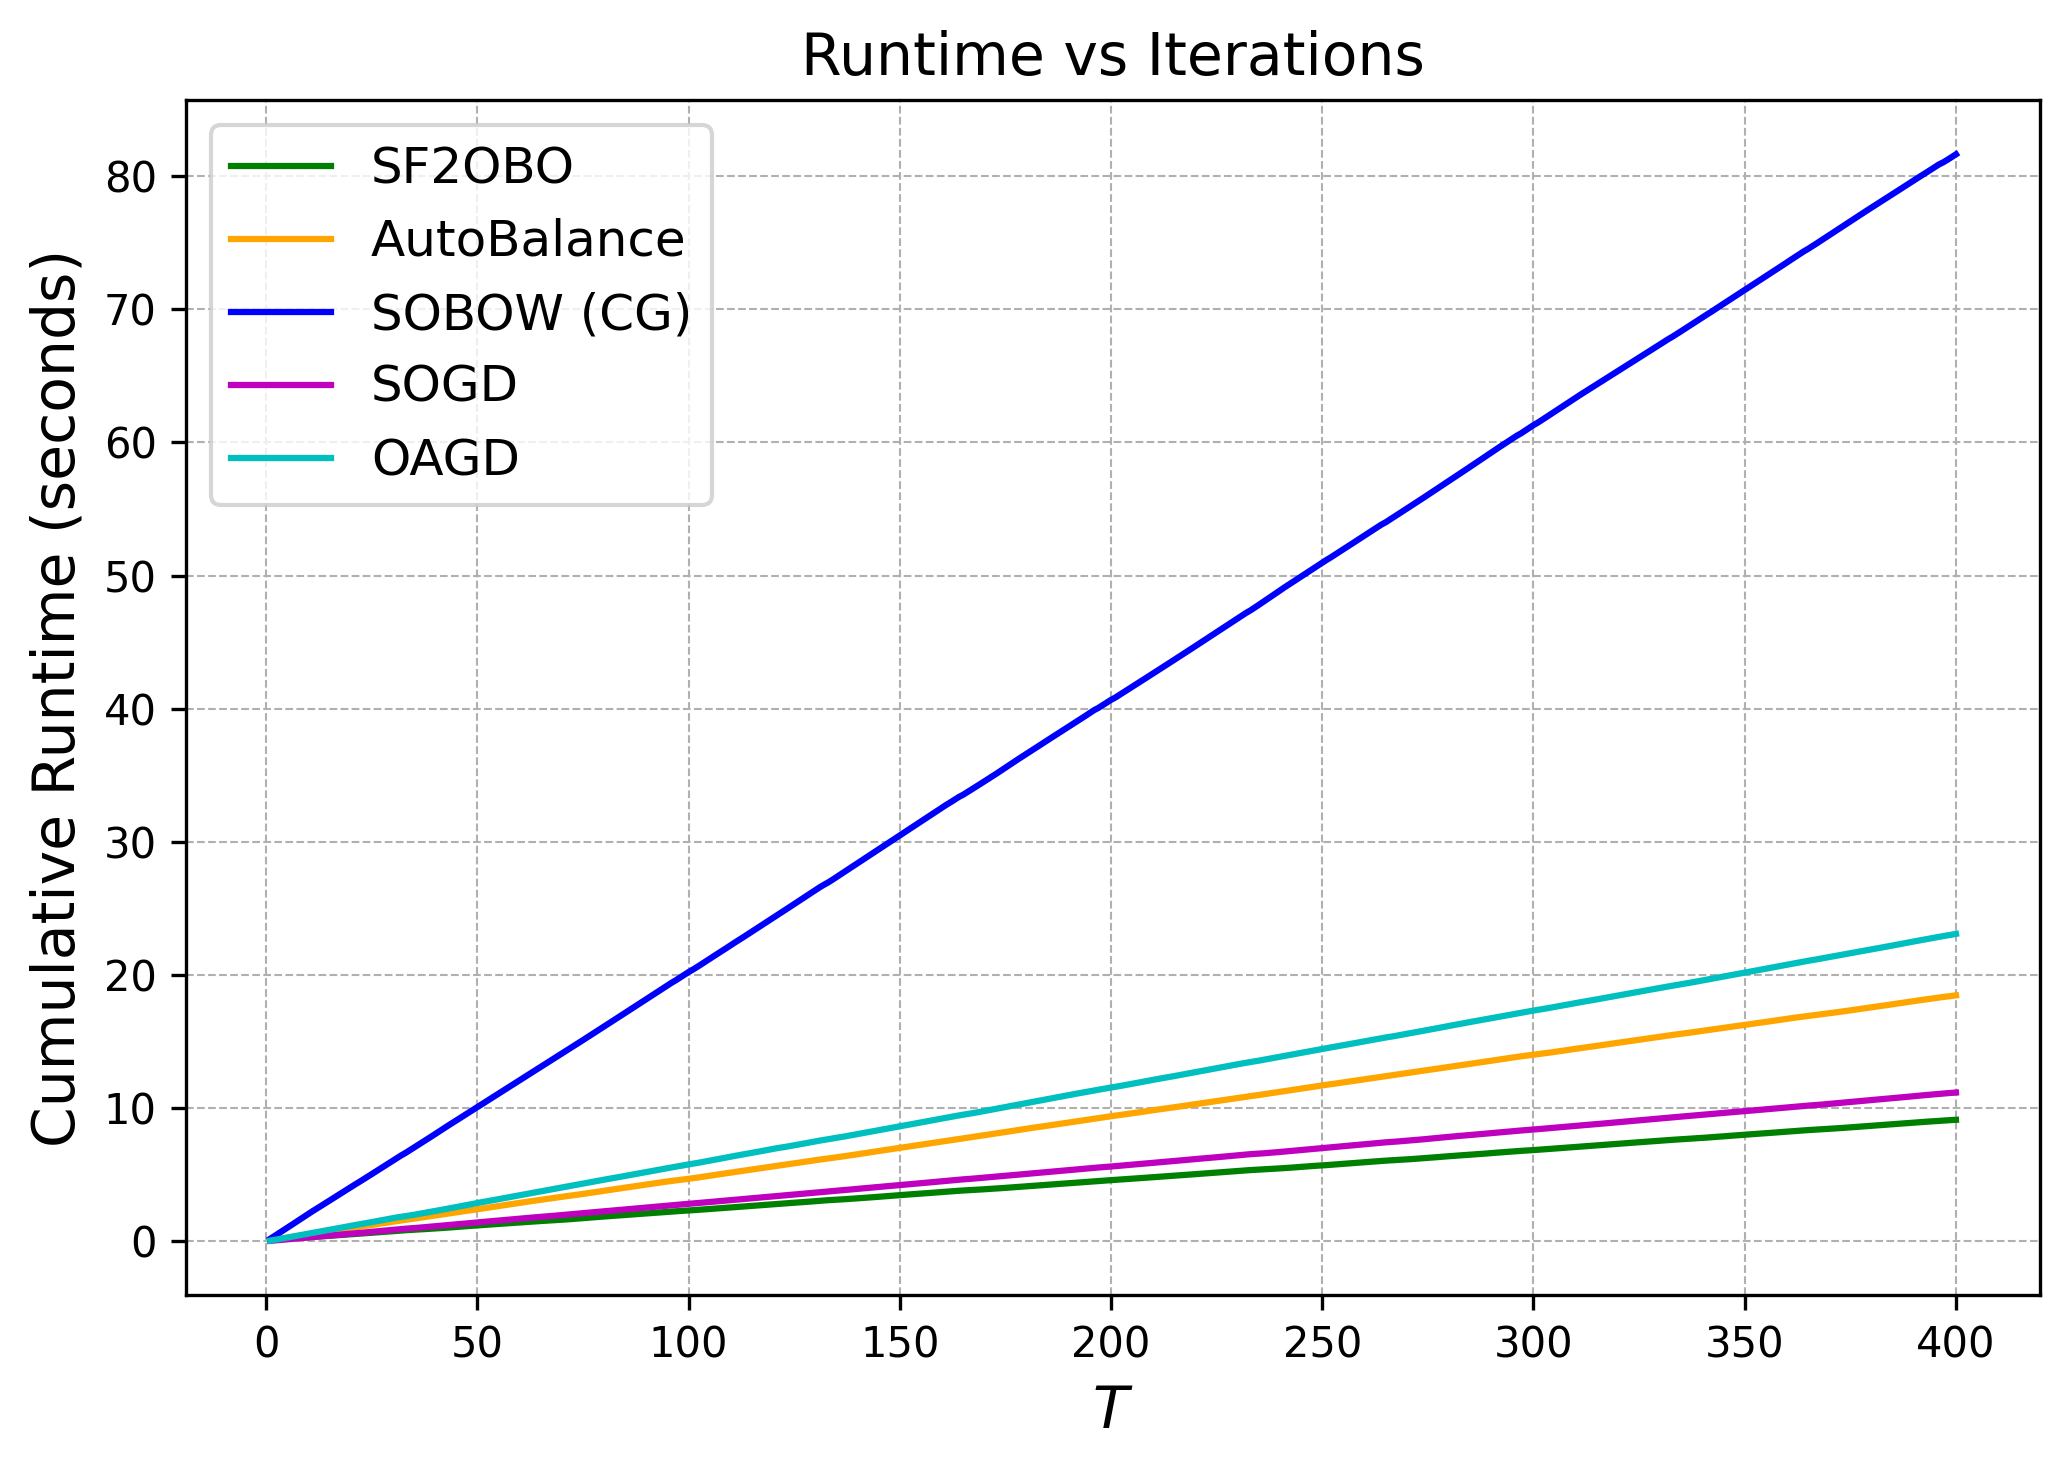
\includegraphics[width=\linewidth]{Plots/time_complexity_vs_iterations_myrun3.png}
    \label{fig:runtime-myrun3}
  \end{subfigure}%  <- no whitespace
  \hfill
  \begin{subfigure}[t]{0.32\linewidth}
    \centering
    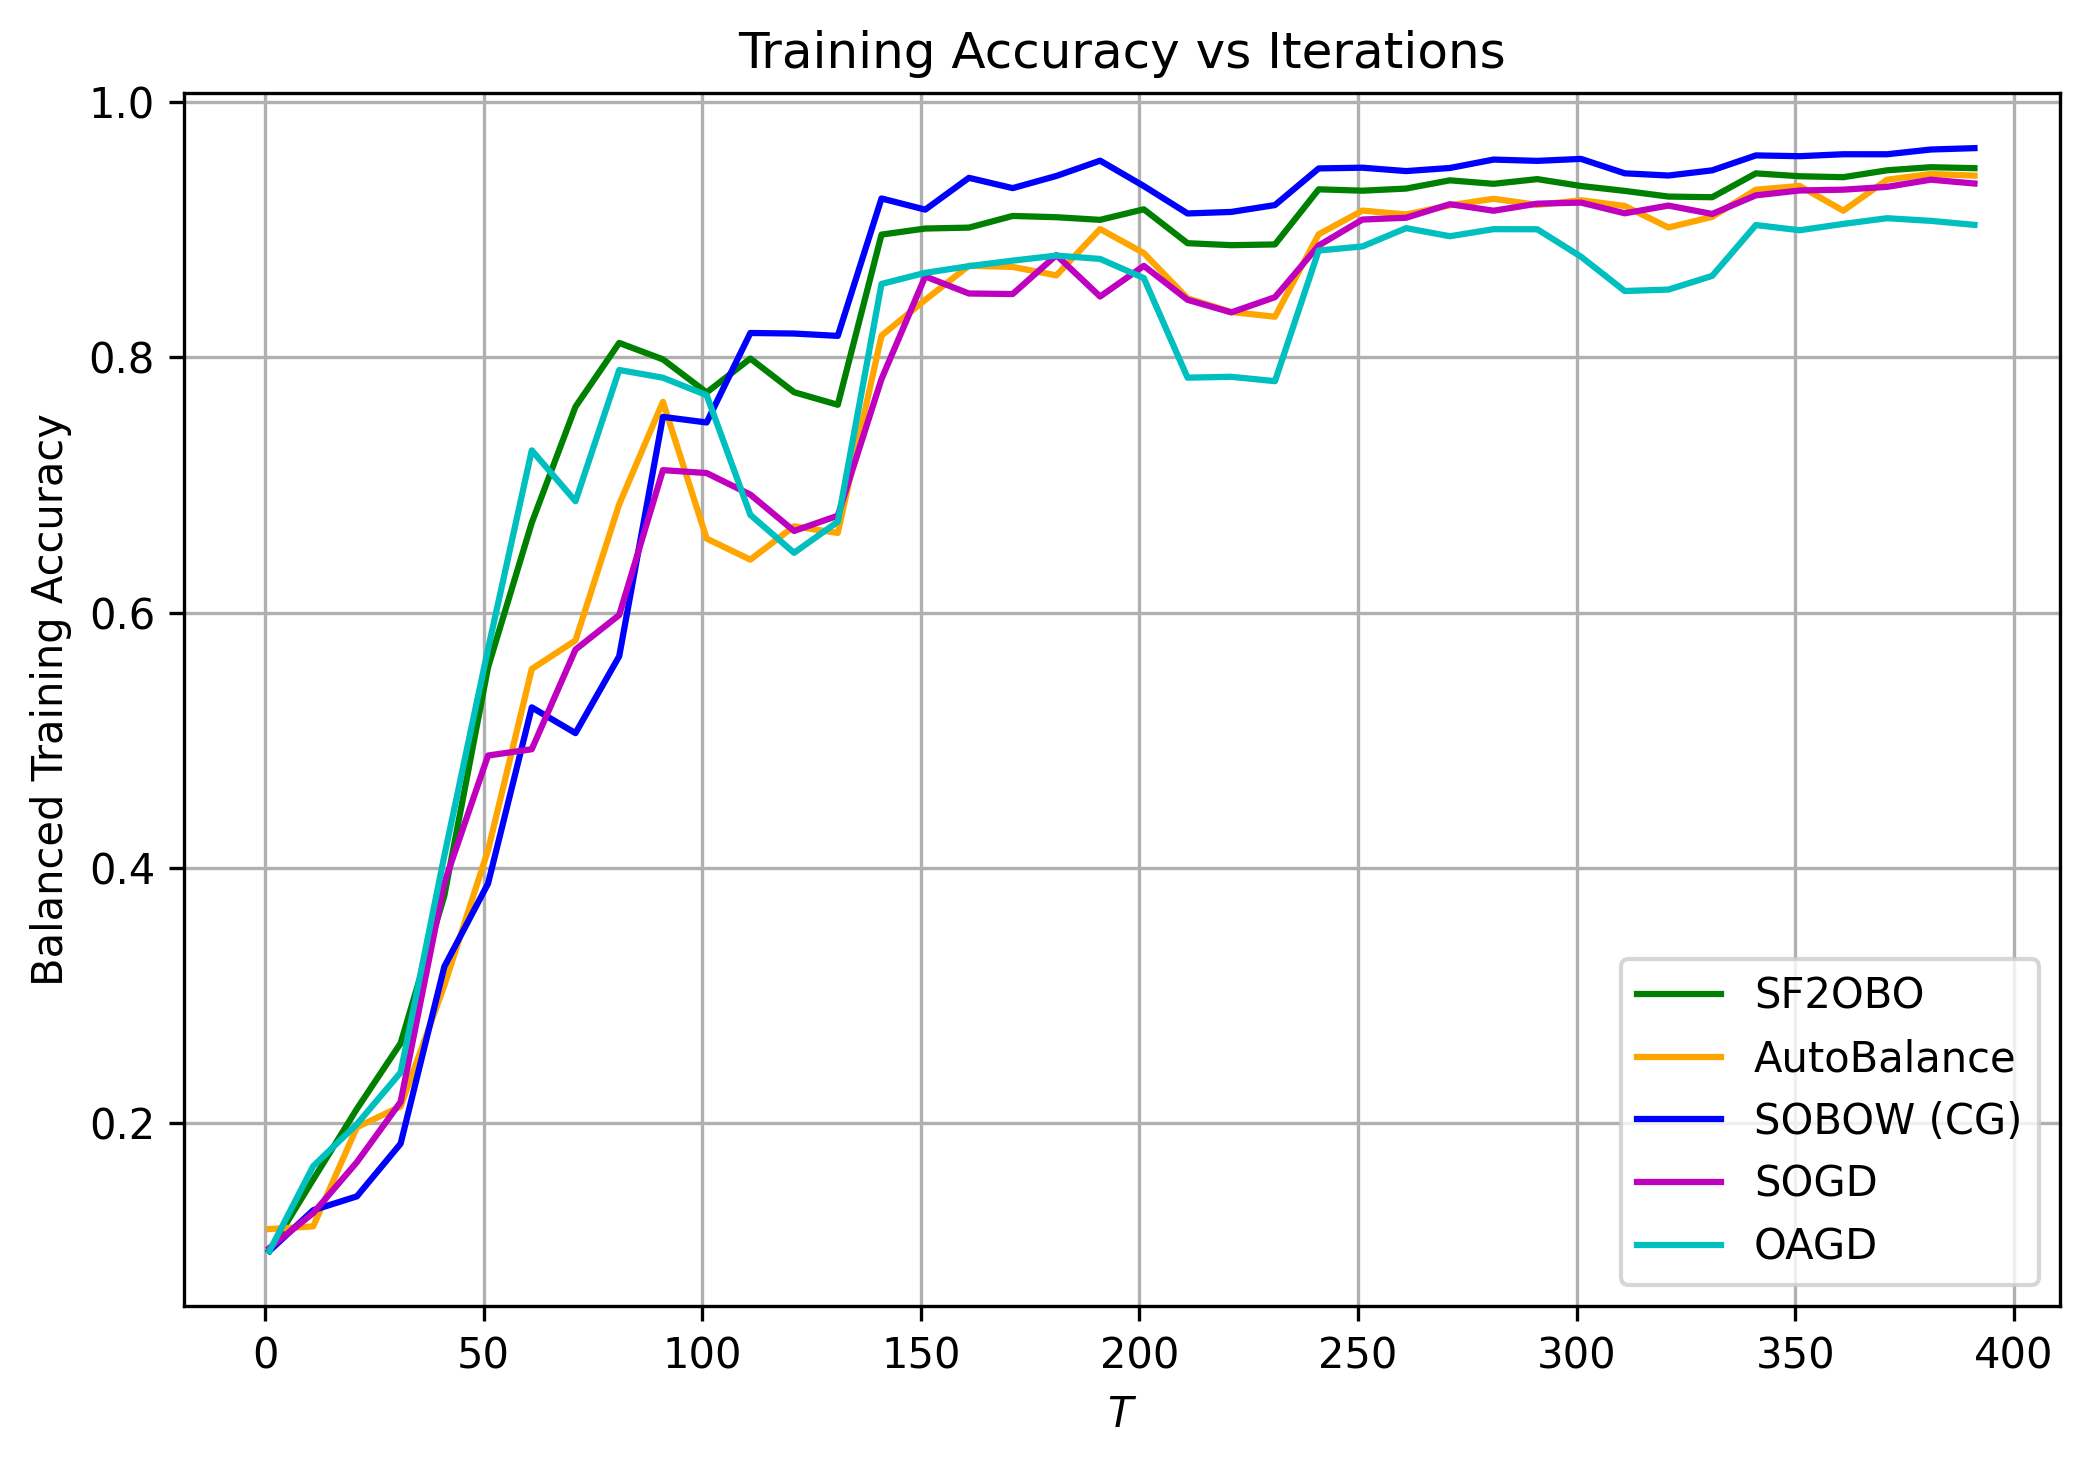
\includegraphics[width=\linewidth]{Plots/accuracy_vs_iterations_myrun32.png}
    \label{fig:trainacc-myrun32}
  \end{subfigure}% 
  \hfill
  \begin{subfigure}[t]{0.32\linewidth}
    \centering
    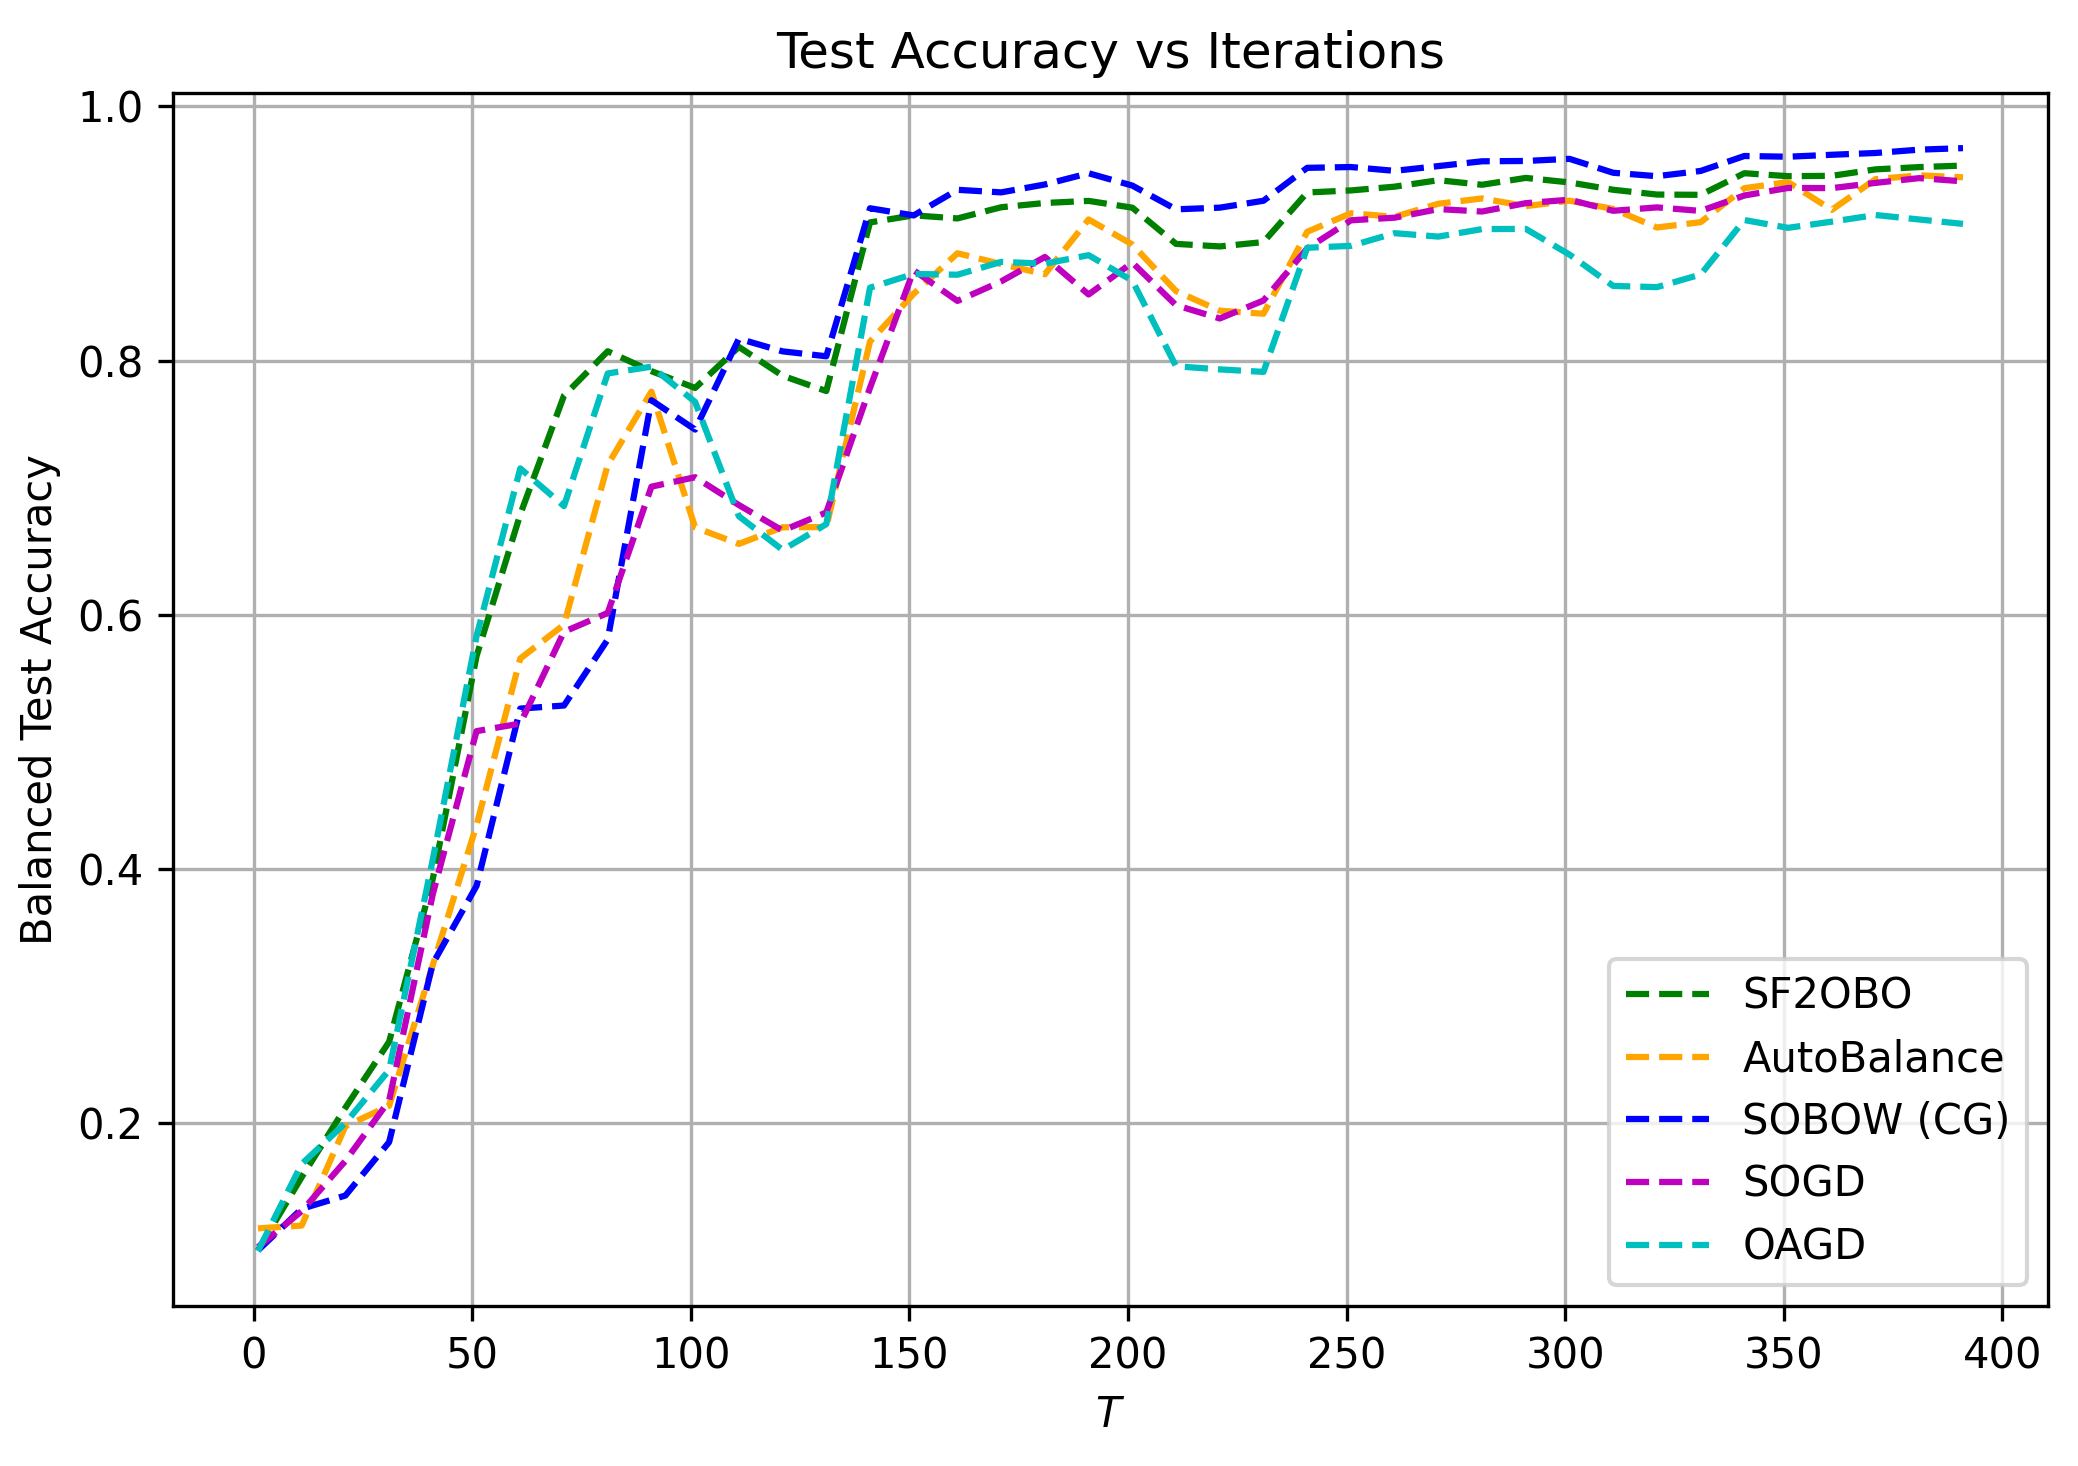
\includegraphics[width=\linewidth]{Plots/accuracy_vs_iterations_myrun31.png}
    \label{fig:testacc-myrun31}
  \end{subfigure}
  \caption{Performance (mean$\pm$std) on online parametric loss tuning with distribution shift on MNIST across five runs, comparing
  OAGD~\citep{tarzanagh2024onlinebileveloptimizationregret}, SOBOW~\citep{lin2023nonconvex}, SOGD~\citep{anonymous2025stochastic},
  AutoBalance~\citep{li2021autobalance} with our stochastic variance-reduced method $\mathrm{VR}\text{--}\mathrm{SF}^2\mathrm{OBO}$.}
  \label{fig:mnist-parametric-imbalance-3up}
\end{figure}
\FloatBarrier  

\begin{table}[!htbp]
  \centering
  \begin{adjustbox}{max width=\linewidth}
  \begin{tabular}{lcccc}
    \toprule
    \textbf{Algorithm\textbackslash Iteration} & \textbf{100} & \textbf{200} & \textbf{300} & \textbf{400} \\
    \midrule
    SOBOW (CG)         & $0.847\!\pm\!0.063$ & $0.947\!\pm\!0.023$ & $0.958\!\pm\!0.005$ & $0.964\!\pm\!0.005$ \\
    \textbf{VR--SF$^2$OBO}        & $\mathbf{0.845\!\pm\!0.048}$ & $\mathbf{0.921\!\pm\!0.023}$ & $\mathbf{0.940\!\pm\!0.004}$ & $\mathbf{0.948\!\pm\!0.006}$ \\
    AutoBalance        & $0.760\!\pm\!0.048$ & $0.891\!\pm\!0.005$ & $0.920\!\pm\!0.027$ & $0.946\!\pm\!0.007$ \\
    SOGD               & $0.764\!\pm\!0.044$ & $0.896\!\pm\!0.010$ & $0.918\!\pm\!0.016$ & $0.931\!\pm\!0.009$ \\
    OAGD               & $0.825\!\pm\!0.054$ & $0.890\!\pm\!0.018$ & $0.903\!\pm\!0.012$ & $0.906\!\pm\!0.008$ \\
    \bottomrule
  \end{tabular}
  \end{adjustbox}
  \caption{Balanced \textbf{train} accuracy (mean$\;\pm\;$std) at iterations 100, 200, 300, and 400 for each algorithm in the \emph{Online Parametric Loss Tuning for Imbalanced Data} experiment.}
  \label{tab:online-parametric-train-mean-std}
\end{table}
\FloatBarrier

\begin{table}[!htbp]
  \centering
  \begin{adjustbox}{max width=\linewidth}
  \begin{tabular}{lcccc}
    \toprule
    \textbf{Algorithm\textbackslash Iteration} & \textbf{100} & \textbf{200} & \textbf{300} & \textbf{400} \\
    \midrule
    SOBOW (CG)         & $0.874\!\pm\!0.050$ & $0.945\!\pm\!0.009$ & $0.960\!\pm\!0.007$ & $0.967\!\pm\!0.003$ \\
    \textbf{VR--SF$^2$OBO}        & $\mathbf{0.849\!\pm\!0.039}$ & $\mathbf{0.927\!\pm\!0.011}$ & $\mathbf{0.945\!\pm\!0.004}$ & $\mathbf{0.952\!\pm\!0.006}$ \\
    AutoBalance        & $0.789\!\pm\!0.048$ & $0.904\!\pm\!0.008$ & $0.921\!\pm\!0.029$ & $0.947\!\pm\!0.002$ \\
    SOGD               & $0.779\!\pm\!0.038$ & $0.896\!\pm\!0.011$ & $0.918\!\pm\!0.014$ & $0.937\!\pm\!0.008$ \\
    OAGD               & $0.820\!\pm\!0.055$ & $0.890\!\pm\!0.003$ & $0.909\!\pm\!0.005$ & $0.913\!\pm\!0.008$ \\
    \bottomrule
  \end{tabular}
  \end{adjustbox}
  \caption{Balanced \textbf{test} accuracy (mean$\;\pm\;$std) at iterations 100, 200, 300, and 400 for each algorithm in the \emph{Online Parametric Loss Tuning for Imbalanced Data} experiment.}
  \label{tab:online-parametric-test-mean-std}
\end{table}
\FloatBarrier



% \section{Conclusion}

\bibliographystyle{abbrvnat}
\bibliography{references}


%%%%%%%%%%%%%%%%%%%%%%%%%%%%%%%%%%%%%%%%%%%%%%%%%%%%%%%%%%%%
\section*{Checklist}


% %%% BEGIN INSTRUCTIONS %%%
The checklist follows the references. For each question, choose your answer from the three possible options: Yes, No, Not Applicable.  You are encouraged to include a justification to your answer, either by referencing the appropriate section of your paper or providing a brief inline description (1-2 sentences). 
Please do not modify the questions.  Note that the Checklist section does not count towards the page limit. Not including the checklist in the first submission won't result in desk rejection, although in such case we will ask you to upload it during the author response period and include it in camera ready (if accepted).
% %%% END INSTRUCTIONS %%%


 \begin{enumerate}


 \item For all models and algorithms presented, check if you include:
 \begin{enumerate}
   \item A clear description of the mathematical setting, assumptions, algorithm, and/or model. [Yes/No/Not Applicable]
   \item An analysis of the properties and complexity (time, space, sample size) of any algorithm. [Yes/No/Not Applicable]
   \item (Optional) Anonymized source code, with specification of all dependencies, including external libraries. [Yes/No/Not Applicable]
 \end{enumerate}


 \item For any theoretical claim, check if you include:
 \begin{enumerate}
   \item Statements of the full set of assumptions of all theoretical results. [Yes/No/Not Applicable]
   \item Complete proofs of all theoretical results. [Yes/No/Not Applicable]
   \item Clear explanations of any assumptions. [Yes/No/Not Applicable]     
 \end{enumerate}


 \item For all figures and tables that present empirical results, check if you include:
 \begin{enumerate}
   \item The code, data, and instructions needed to reproduce the main experimental results (either in the supplemental material or as a URL). [Yes/No/Not Applicable]
   \item All the training details (e.g., data splits, hyperparameters, how they were chosen). [Yes/No/Not Applicable]
         \item A clear definition of the specific measure or statistics and error bars (e.g., with respect to the random seed after running experiments multiple times). [Yes/No/Not Applicable]
         \item A description of the computing infrastructure used. (e.g., type of GPUs, internal cluster, or cloud provider). [Yes/No/Not Applicable]
 \end{enumerate}

 \item If you are using existing assets (e.g., code, data, models) or curating/releasing new assets, check if you include:
 \begin{enumerate}
   \item Citations of the creator If your work uses existing assets. [Yes/No/Not Applicable]
   \item The license information of the assets, if applicable. [Yes/No/Not Applicable]
   \item New assets either in the supplemental material or as a URL, if applicable. [Yes/No/Not Applicable]
   \item Information about consent from data providers/curators. [Yes/No/Not Applicable]
   \item Discussion of sensible content if applicable, e.g., personally identifiable information or offensive content. [Yes/No/Not Applicable]
 \end{enumerate}

 \item If you used crowdsourcing or conducted research with human subjects, check if you include:
 \begin{enumerate}
   \item The full text of instructions given to participants and screenshots. [Yes/No/Not Applicable]
   \item Descriptions of potential participant risks, with links to Institutional Review Board (IRB) approvals if applicable. [Yes/No/Not Applicable]
   \item The estimated hourly wage paid to participants and the total amount spent on participant compensation. [Yes/No/Not Applicable]
 \end{enumerate}

 \end{enumerate}
\appendix
\section{Appendix}

\section{Notation and Assumptions (Glossary)}
\section{Proofs for Offline Ingredients}
Let $y^{*}_{\lambda,t}(x)\in\argmin_y f_t(x,y)+\lambda\big(g_t(x,y)-g_t^{*}(x)\big)$. The offline paper shows \citep[Lemma~4.1]{ChenMaZhang2025}:
\begin{lemma}\label{lem:offline-keys}
Under Assumption~\ref{ass:offline} and $\lambda\ge 2L_f/\mu$, there exist constants $D_1,L_x=O(\ell\kappa^3)$ such that, for all $x$ and each $t$,
\[
\norm{\nabla L^{*}_{\lambda,t}(x)-\nabla\phi_t(x)}\ \le\ \frac{D_1}{\lambda},
\qquad \nabla L^{*}_{\lambda,t}\text{ is }L_x\text{-Lipschitz in }x.
\]
Moreover,
\[
\nabla L^{*}_{\lambda,t}(x)
=\nabla_x f_t\big(x,y^{*}_{\lambda,t}(x)\big)
+\lambda\!\left(\nabla_x g_t\big(x,y^{*}_{\lambda,t}(x)\big)-\nabla_x g_t\big(x,y_t^{*}(x)\big)\right).
\]
\end{lemma}

Finally, $y^{*}_t(x)$ and $y^{*}_{\lambda,t}(x)$ are Lipschitz in $x$ with constants $L_g/\mu$ and $4L_g/\mu$, respectively (Appendix~B in \cite{ChenMaZhang2025}).

\begin{lemma}
\label{lem:B1}
Under \Cref{ass:offline}, for $\lambda \ge 2L_f/\mu$, the function
\[
y \ \longmapsto \ L_{\lambda,t}(x,y)\ :=\ f_{t}(x,y)+\lambda\,g_{t}(x,y)
\]
is $(\lambda\mu/2)$-strongly convex (in $y$).
\end{lemma}

\begin{proof}
Fix $x$. By \Cref{ass:offline}, $g_{t}(x,\cdot)$ is $\mu$-strongly convex, hence
$\nabla^2_{yy} g_{t}(x,y) \succeq \mu I$ for all $y$. By Assumption~\ref{ass:offline}(A2), $\nabla f_{t}$ is
$L_f$-Lipschitz in $(x,y)$ and hence in $y$; since $f_{t}$ is twice continuously differentiable, we have
$\|\nabla^2_{yy} f_{t}(x,y)\|\le L_f$ for all $y$, which implies
$\nabla^2_{yy} f_{t}(x,y) \succeq -\,L_f I$.

Therefore, for any $y$ and any $v\in\mathbb{R}^{d_y}$,
\[
v^\top \nabla^2_{yy} L_{\lambda,t}(x,y)\, v
= v^\top\!\Big(\nabla^2_{yy} f_{t}(x,y)+\lambda\,\nabla^2_{yy} g_{t}(x,y)\Big) v
\ \ge\ (-L_f+\lambda\mu)\,\|v\|^2.
\]
Equivalently, $\nabla^2_{yy} L_{\lambda,t}(x,y) \succeq (\lambda\mu-L_f) I$ for all $y$.
If $\lambda \ge 2L_f/\mu$, then $\lambda\mu-L_f \ge \tfrac{1}{2}\lambda\mu$, which
shows that $L_{\lambda,t}(x,\cdot)$ is $(\lambda\mu/2)$-strongly convex.
\end{proof}
\begin{lemma}
\label{lem:B2}
Under \Cref{ass:offline}, for $\lambda \ge 2L_f/\mu$, it holds that
\[
\bigl\|y^*_{\lambda,t}(x) - y^*_{t}(x)\bigr\| \;\le\; \frac{C_f}{\lambda\,\mu}.
\]
\end{lemma}
\begin{proof}
By the first-order optimality condition, we have
\[
\nabla_y f_{t}\bigl(x, y^*_{\lambda,t}(x)\bigr) + \lambda \nabla_y g_{t}\bigl(x, y^*_{\lambda,t}(x)\bigr) \;=\; 0.
\]
Therefore,
\[
\bigl\|y^*_{\lambda,t}(x) - y^*_{t}(x)\bigr\|
\;\le\; \frac{1}{\mu}\,\bigl\|\nabla_y g_{t}\bigl(x, y^*_{\lambda,t}(x)\bigr)\bigr\|
\;=\; \frac{1}{\lambda\,\mu}\,\bigl\|\nabla_y f_{t}\bigl(x, y^*_{\lambda,t}(x)\bigr)\bigr\|
\;\le\; \frac{C_f}{\lambda\,\mu}.
\]
\end{proof}


\begin{lemma}
\label{lem:B3}
Under \Cref{ass:offline}, for any $\lambda \ge 2L_f/\mu$, it holds that
\[
\bigl|\,L^*_{\lambda,t}(x) - \varphi_{t}(x)\,\bigr| \;\le\; \frac{D_0}{\lambda},
\qquad\text{where}\qquad
D_0 := \Bigl(C_f + \frac{C_f L_g}{2\mu}\Bigr)\frac{C_f}{\mu}
= \mathcal{O}(\ell\,\kappa^2).
\]
\end{lemma}

\begin{proof}
By definition,
\[
\bigl|L^*_{\lambda,t}(x) - \varphi_{t}(x)\bigr|
= \bigl|\,f_{t}\bigl(x,y^*_{\lambda,t}(x)\bigr) - f_{t}\bigl(x,y^*_{t}(x)\bigr)\,\bigr|
  \;+\; \lambda\,\bigl|\,g_{t}\bigl(x,y^*_{\lambda,t}(x)\bigr) - g_{t}\bigl(x,y^*_{t}(x)\bigr)\,\bigr|.
\]
Since $f_{t}$ is $C_f$-Lipschitz in $y$,
\[
\bigl|\,f_{t}\bigl(x,y^*_{\lambda,t}(x)\bigr) - f_{t}\bigl(x,y^*_{t}(x)\bigr)\,\bigr|
\;\le\; C_f\,\bigl\|y^*_{\lambda,t}(x) - y^*_{t}(x)\bigr\|.
\]
Because $\nabla_y g_{t}$ is $L_g$-Lipschitz and $\nabla_y g_{t}\bigl(x,y^*_{t}(x)\bigr)=0$,
the descent lemma gives
\[
\bigl|\,g_{t}\bigl(x,y^*_{\lambda,t}(x)\bigr) - g_{t}\bigl(x,y^*_{t}(x)\bigr)\,\bigr|
\;\le\; \frac{L_g}{2}\,\bigl\|y^*_{\lambda,t}(x) - y^*_{t}(x)\bigr\|^2.
\]
Combining the two bounds yields
\[
\bigl|L^*_{\lambda,t}(x) - \varphi_{t}(x)\bigr|
\;\le\; C_f\,\bigl\|y^*_{\lambda,t}(x) - y^*_{t}(x)\bigr\|
\;+\; \lambda\,\frac{L_g}{2}\,\bigl\|y^*_{\lambda,t}(x) - y^*_{t}(x)\bigr\|^2.
\]
By \Cref{lem:B2}, $\|y^*_{\lambda,t}(x) - y^*_{t}(x)\| \le C_f/(\lambda\mu)$. Substituting this,
\[
\bigl|L^*_{\lambda,t}(x) - \varphi_{t}(x)\bigr|
\;\le\; C_f\cdot \frac{C_f}{\lambda\mu}
\;+\; \lambda\cdot \frac{L_g}{2}\cdot \Bigl(\frac{C_f}{\lambda\mu}\Bigr)^2
\;=\; \frac{1}{\lambda}\,\Bigl(C_f + \frac{C_f L_g}{2\mu}\Bigr)\frac{C_f}{\mu}.
\]
This is exactly the claimed bound with $D_0 := \bigl(C_f + \tfrac{C_f L_g}{2\mu}\bigr)\tfrac{C_f}{\mu}
= \mathcal{O}(\ell\,\kappa^2)$, where $\ell=\max\{C_f,L_f,L_g,\rho_g\}$ and $\kappa=\ell/\mu$.
\end{proof}
\begin{lemma}
\label{lem:B4}
Under \Cref{ass:offline}, for $\lambda \ge 2L_f/\mu$, it holds that
\[
\bigl\|\nabla L^*_{\lambda,t}(x) - \nabla \varphi_{t}(x)\bigr\| \;\le\; \frac{D_1}{\lambda},
\]
where
\[
D_1 \;:=\;
\Bigl(
L_f + \frac{\rho_g L_g}{\mu}
+ \frac{C_f L_g \rho_g}{2\mu^2}
+ \frac{C_f \rho_g}{2\mu}
\Bigr)\frac{C_f}{\mu}
\;=\; \mathcal{O}(\ell\,\kappa^3).
\]
\end{lemma}

\begin{proof}
Taking total derivative of $\varphi_{t}(x)=f_{t}\bigl(x,y^*_{t}(x)\bigr)$ gives
\[
\nabla \varphi_{t}(x)
= \nabla_x f_{t}\bigl(x,y^*_{t}(x)\bigr)
- \nabla^2_{xy} g_{t}\bigl(x,y^*_{t}(x)\bigr)\,[\nabla^2_{yy} g_{t}\bigl(x,y^*_{t}(x)\bigr)]^{-1}\,\nabla_y f_{t}\bigl(x,y^*_{t}(x)\bigr).
\]
Also,
\[
\nabla L^*_{\lambda,t}(x)
= \nabla_x f_{t}\bigl(x,y^*_{\lambda,t}(x)\bigr)
+ \lambda\Bigl(\nabla_x g_{t}\bigl(x,y^*_{\lambda,t}(x)\bigr) - \nabla_x g_{t}\bigl(x,y^*_{t}(x)\bigr)\Bigr).
\]
Hence,
\begin{align*}
\nabla L^*_{\lambda,t}(x) - \nabla \varphi_{t}(x)
&= \underbrace{\nabla_x f_{t}\bigl(x,y^*_{\lambda,t}(x)\bigr) - \nabla_x f_{t}\bigl(x,y^*_{t}(x)\bigr)}_{\text{(A)}} \\
&\quad + \underbrace{\nabla^2_{xy} g_{t}\bigl(x,y^*_{t}(x)\bigr)\,[\nabla^2_{yy} g_{t}\bigl(x,y^*_{t}(x)\bigr)]^{-1}\Bigl(\nabla_y f_{t}\bigl(x,y^*_{t}(x)\bigr)-\nabla_y f_{t}\bigl(x,y^*_{\lambda,t}(x)\bigr)\Bigr)}_{\text{(B)}} \\
&\quad + \underbrace{\lambda\,\nabla^2_{xy} g_{t}\bigl(x,y^*_{t}(x)\bigr)\,[\nabla^2_{yy} g_{t}\bigl(x,y^*_{t}(x)\bigr)]^{-1} \Bigl(\nabla^2_{yy} g_{t}\bigl(x,y^*_{t}(x)\bigr)\,(y^*_{\lambda,t}(x)-y^*_{t}(x))}_{\text{(C)}}\\
&\qquad\qquad\quad \qquad\qquad\qquad\qquad\underbrace{ + \nabla_y g_{t}\bigl(x,y^*_{t}(x)\bigr) - \nabla_y g_{t}\bigl(x,y^*_{\lambda,t}(x)\bigr)\Bigr)}_{\text{(C, cont.)}} \\
&\quad + \underbrace{\lambda\Bigl(\nabla_x g_{t}\bigl(x,y^*_{\lambda,t}(x)\bigr)-\nabla_x g_{t}\bigl(x,y^*_{t}(x)\bigr) - \nabla^2_{xy} g_{t}\bigl(x,y^*_{t}(x)\bigr)\,(y^*_{\lambda,t}(x)-y^*_{t}(x))\Bigr)}_{\text{(D)}}.
\end{align*}
Taking norms and using the smoothness/curvature constants in \Cref{ass:offline},
\[
\|\text{(A)}\| \le L_f\|y^*_{\lambda,t}(x)-y^*_{t}(x)\|,\quad
\|\text{(B)}\| \le \frac{\rho_g L_g}{\mu}\|y^*_{\lambda,t}(x)-y^*_{t}(x)\|.
\]
For the quadratic remainders,
\[
\|\text{(C)}\| \le \frac{\lambda L_g \rho_g}{2\mu}\|y^*_{\lambda,t}(x)-y^*_{t}(x)\|^2,\qquad
\|\text{(D)}\| \le \frac{\lambda \rho_g}{2}\|y^*_{\lambda,t}(x)-y^*_{t}(x)\|^2.
\]
By \Cref{lem:B2}, $\|y^*_{\lambda,t}(x)-y^*_{t}(x)\|\le C_f/(\lambda\mu)$. Substituting this bound into the
four terms above yields
\[
\|\nabla L^*_{\lambda,t}(x) - \nabla \varphi_{t}(x)\|
\;\le\;
\Bigl(
L_f + \frac{\rho_g L_g}{\mu}
+ \frac{C_f L_g \rho_g}{2\mu^2}
+ \frac{C_f \rho_g}{2\mu}
\Bigr)\frac{C_f}{\lambda\mu}
= \frac{D_1}{\lambda},
\]
which proves the claim.
\end{proof}
\begin{lemma}
\label{lem:B5}
Under \Cref{ass:offline}, for $\lambda \ge 2L_f/\mu$, it holds that
\[
\bigl\|\nabla y^*_{t}(x) - \nabla y^*_{\lambda,t}(x)\bigr\| \;\le\; \frac{D_2}{\lambda},
\qquad
D_2 \;:=\; \Bigl(\frac{1}{\mu} + \frac{2L_g}{\mu^2}\Bigr)\Bigl(L_f + \frac{C_f\rho_g}{\mu}\Bigr)
\;=\; \mathcal{O}(\kappa^3).
\]
\end{lemma}
\begin{proof}
Differentiating the first-order condition $\nabla_y g_{t}\bigl(x,y^*_{t}(x)\bigr)=0$ w.r.t.\ $x$ gives
\begin{align}\label{eq_004}
\nabla^2_{xy} g_{t}\bigl(x,y^*_{t}(x)\bigr) \;+\; \nabla y^*_{t}(x)\,\nabla^2_{yy} g_{t}\bigl(x,y^*_{t}(x)\bigr) \;=\; 0.
\end{align}
Rearranging yields the closed form
\begin{align}\label{eq_005}
\nabla y^*_{t}(x) \;=\; -\,\nabla^2_{xy} g_{t}\bigl(x,y^*_{t}(x)\bigr)\bigl[\nabla^2_{yy} g_{t}\bigl(x,y^*_{t}(x)\bigr)\bigr]^{-1}. 
\end{align}
Similarly, since $y^*_{\lambda,t}(x)$ minimizes $L_{\lambda,t}(x,\cdot)=f_{t}(x,\cdot)+\lambda g_{t}(x,\cdot)$,
\begin{align}\label{eq_006}
\nabla y^*_{\lambda,t}(x) \;=\; -\,\nabla^2_{xy} L_{\lambda,t}\bigl(x,y^*_{\lambda,t}(x)\bigr)
\bigl[\nabla^2_{yy} L_{\lambda,t}\bigl(x,y^*_{\lambda,t}(x)\bigr)\bigr]^{-1}.
\end{align}
Using the identity $A^{-1}-B^{-1}=A^{-1}(B-A)B^{-1}$ and the strong convexity in $y$,
we first bound the difference of the inverses:
\[
\Bigl\|
\bigl[\nabla^2_{yy}g_{t}(x,y^*_{t}(x))\bigr]^{-1}
-\Bigl[\frac{1}{\lambda}\nabla^2_{yy}L_{\lambda,t}\bigl(x,y^*_{\lambda,t}(x)\bigr)\Bigr]^{-1}
\Bigr\|
\;\le\; \frac{2}{\lambda \mu^2}\Bigl(L_f + \frac{C_f\rho_g}{\mu}\Bigr),
\]
where we used $\|\nabla^2_{yy}f_{t}\| \le L_f$, the $\rho_g$-Lipschitzness of $\nabla^2 g_{t}$ in $y$,
and \Cref{lem:B2}: $\|y^*_{\lambda,t}(x)-y^*_{t}(x)\| \le C_f/(\lambda\mu)$. 

Now normalize \Cref{eq_004,eq_005} by $\lambda$ for comparison and apply the triangle inequality:
\begin{align*}
\|\nabla y^*_{\lambda,t}(x)-\nabla y^*_{t}(x)\|
&\le \Bigl\|\nabla^2_{xy}g_{t}\bigl(x,y^*_{t}(x)\bigr)-\frac{1}{\lambda}\nabla^2_{xy}L_{\lambda,t}\bigl(x,y^*_{\lambda,t}(x)\bigr)\Bigr\|
\cdot \bigl\|[\nabla^2_{yy}g_{t}(x,y^*_{t}(x))]^{-1}\bigr\|\\
&\quad + \Bigl\|\frac{1}{\lambda}\nabla^2_{xy}L_{\lambda,t}\bigl(x,y^*_{\lambda,t}(x)\bigr)\Bigr\|
\cdot \Bigl\|[\nabla^2_{yy}g_{t}(x,y^*_{t}(x))]^{-1}-\Bigl[\frac{1}{\lambda}\nabla^2_{yy}L_{\lambda,t}\bigl(x,y^*_{\lambda,t}(x)\bigr)\Bigr]^{-1}\Bigr\|.
\end{align*}
The first factor is bounded by
\[
\frac{1}{\mu}\Bigl(\frac{L_f}{\lambda} + \rho_g\|y^*_{\lambda,t}(x)-y^*_{t}(x)\|\Bigr)
\;\le\; \frac{1}{\lambda\mu}\Bigl(L_f + \frac{C_f\rho_g}{\mu}\Bigr),
\]
using again \Cref{lem:B2}. For the second factor, from $\lambda \ge 2L_f/\mu$ we have
$\bigl\|\tfrac{1}{\lambda}\nabla^2_{xy}L_{\lambda,t}(\cdot,\cdot)\bigr\|\!\le\! 2L_g$, which combined with \eqref{eq_006}
yields
\[
\Bigl\|\frac{1}{\lambda}\nabla^2_{xy}L_{\lambda,t}\bigl(x,y^*_{\lambda,t}(x)\bigr)\Bigr\|
\cdot
\Bigl\|[\nabla^2_{yy}g_{t}(\cdot)]^{-1}-\Bigl[\tfrac{1}{\lambda}\nabla^2_{yy}L_{\lambda,t}(\cdot)\Bigr]^{-1}\Bigr\|
\;\le\; \frac{2L_g}{\lambda\mu^2}\Bigl(L_f + \frac{C_f\rho_g}{\mu}\Bigr).
\]
Putting the two bounds together gives
\[
\|\nabla y^*_{\lambda,t}(x)-\nabla y^*_{t}(x)\|
\;\le\; \Bigl(\frac{1}{\lambda\mu} + \frac{2L_g}{\lambda\mu^2}\Bigr)\Bigl(L_f + \frac{C_f\rho_g}{\mu}\Bigr)
\;=\; \frac{D_2}{\lambda},
\]
which proves the claim.
\end{proof}
\begin{lemma}
\label{lem:B6}
Under \Cref{ass:offline}, for $\lambda \ge 2L_f/\mu$, it holds that
\[
\bigl\|\nabla y^*_{\lambda,t}(x)\bigr\| \;\le\; \frac{4L_g}{\mu}.
\]
\end{lemma}

\begin{proof}
Since $y^*_{\lambda,t}(x)$ minimizes $L_{\lambda,t}(x,\cdot)=f_{t}(x,\cdot)+\lambda g_{t}(x,\cdot)$, the
first-order optimality condition $\nabla_y L_{\lambda,t}\bigl(x,y^*_{\lambda,t}(x)\bigr)=0$
and the implicit function theorem give
\[
\nabla y^*_{\lambda,t}(x)
= -\,\nabla^2_{xy} L_{\lambda,t}\bigl(x,y^*_{\lambda,t}(x)\bigr)\,
\Bigl[\nabla^2_{yy} L_{\lambda,t}\bigl(x,y^*_{\lambda,t}(x)\bigr)\Bigr]^{-1}.
\]
Taking operator norms yields
\[
\bigl\|\nabla y^*_{\lambda,t}(x)\bigr\|
\;\le\; \bigl\|\nabla^2_{xy} L_{\lambda,t}\bigl(x,y^*_{\lambda,t}(x)\bigr)\bigr\|\;
\Bigl\|\Bigl[\nabla^2_{yy} L_{\lambda,t}\bigl(x,y^*_{\lambda,t}(x)\bigr)\Bigr]^{-1}\Bigr\|.
\]
By smoothness, $\|\nabla^2_{xy} L_{\lambda,t}(\cdot,\cdot)\|
\le \|\nabla^2_{xy} f_{t}(\cdot,\cdot)\|+\lambda\|\nabla^2_{xy} g_{t}(\cdot,\cdot)\|
\le L_f+\lambda L_g \le 2\lambda L_g$ when $\lambda \ge 2L_f/\mu$.
Moreover, by \Cref{lem:B1}, $L_{\lambda,t}(x,\cdot)$ is $(\lambda\mu/2)$-strongly convex, so
$\nabla^2_{yy} L_{\lambda,t}(\cdot,\cdot) \succeq (\lambda\mu/2)I$ and hence
$\bigl\|\bigl[\nabla^2_{yy} L_{\lambda,t}(\cdot,\cdot)\bigr]^{-1}\bigr\| \le 2/(\lambda\mu)$.
Combining the two bounds gives
\[
\bigl\|\nabla y^*_{\lambda,t}(x)\bigr\| \;\le\; (2\lambda L_g)\cdot\frac{2}{\lambda\mu}
\;=\; \frac{4L_g}{\mu}.
\]
\end{proof}

\begin{lemma}[Smoothness of $L^*_{\lambda,t}(x)$]
\label{lem:B7}
Under \Cref{ass:offline}, for $\lambda \ge 2L_f/\mu$, the mapping $\nabla L^*_{\lambda,t}(x)$ is $D_3$-Lipschitz, where
\[
D_3 \;:=\; L_f \;+\; \frac{4L_fL_g}{\mu} \;+\; \frac{C_f\rho_g}{\mu} \;+\; \frac{C_f L_g \rho_g}{\mu^2} \;+\; L_g D_2
\;=\; \mathcal{O}(\ell\kappa^3),
\]
and $D_2$ is the constant from \Cref{lem:B5}.
\end{lemma}

\begin{proof}
Decompose
\begin{align}
    \nabla L^*_{\lambda,t}(x)
= \underbrace{\nabla_x f_{t}\bigl(x,y^*_{\lambda,t}(x)\bigr)}_{=:A(x)}
\;+\;
\underbrace{\lambda\bigl(\nabla_x g_{t}\bigl(x,y^*_{\lambda,t}(x)\bigr)-\nabla_x g_{t}\bigl(x,y^*_{t}(x)\bigr)\bigr)}_{=:B(x)}.
\end{align}
By \Cref{lem:B6}, $y^*_{\lambda,t}(x)$ is $(4L_g/\mu)$-Lipschitz. Therefore $A(x)$ is
$\bigl(1+\tfrac{4L_g}{\mu}\bigr)L_f$-Lipschitz (chain rule with the $L_f$-smoothness of $f_{t}$).

For $B(x)$, take the total derivative:
\begin{align}
    \nabla B(x)
&= \lambda\bigl(\nabla^2_{xx} g_{t}(x,y^*_{\lambda,t}(x))-\nabla^2_{xx} g_{t}(x,y^*_{t}(x))\bigr) \\
&\quad + \lambda\bigl(\nabla y^*_{\lambda,t}(x)\,\nabla^2_{yx} g_{t}(x,y^*_{\lambda,t}(x)) - \nabla y^*_{t}(x)\,\nabla^2_{yx} g_{t}(x,y^*_{t}(x))\bigr).
\end{align}
Hence
\begin{align}
    \|\nabla B(x)\|
&\le \lambda\|\nabla^2_{xx}g_{t}(x,y^*_{\lambda,t})-\nabla^2_{xx}g(x,y^*_{t})\|
 + \lambda\|\nabla y^*_{t}(x)\|\,\|\nabla^2_{yx}g_{t}(x,y^*_{\lambda,t})-\nabla^2_{yx}g_{t}(x,y^*_{t})\| \\
&\qquad + \lambda\|\nabla y^*_{\lambda,t}(x)-\nabla y^*_{t}(x)\|\,\|\nabla^2_{yx}g_{t}(x,y^*_{\lambda,t})\| \\
&\le \lambda\rho_g\!\left(1+\frac{L_g}{\mu}\right)\!\|y^*_{\lambda,t}(x)-y^*_{t}(x)\|
      + \lambda L_g\,\|\nabla y^*_{\lambda,t}(x)-\nabla y^*_{t}(x)\|, 
\end{align}
where we used $\|\nabla y^*_{t}(x)\|\le L_g/\mu$ and the $y$-Lipschitzness ($\rho_g$) of
$\nabla^2 g_{t}$, together with $\|\nabla^2_{yx}g_{t}\|\le L_g$.

Applying \Cref{lem:B2}, $\|y^*_{\lambda,t}(x)-y^*_{t}(x)\|\le C_f/(\lambda\mu)$, and \Cref{lem:B5},
$\|\nabla y^*_{\lambda,t}(x)-\nabla y^*_{t}(x)\|\le D_2/\lambda$, we obtain
\[
\|\nabla B(x)\| \;\le\; \left(1+\frac{L_g}{\mu}\right)\frac{C_f\rho_g}{\mu} \;+\; L_g D_2,
\]
so $B(x)$ is $\bigl( (1+L_g/\mu)\,C_f\rho_g/\mu + L_g D_2 \bigr)$-Lipschitz. 

Combining the Lipschitz constants of $A$ and $B$ yields
\[
D_3 \;=\; \Bigl(1+\frac{4L_g}{\mu}\Bigr)L_f
\;+\; \Bigl(1+\frac{L_g}{\mu}\Bigr)\frac{C_f\rho_g}{\mu} \;+\; L_g D_2
\;=\; L_f + \frac{4L_fL_g}{\mu} + \frac{C_f\rho_g}{\mu} + \frac{C_f L_g \rho_g}{\mu^2} + L_g D_2,
\]
which proves the claim.
\end{proof}
\begin{lemma}\label{lem:descent_phi}
Let $L_{\phi}=\mathcal{O}(\kappa^{3}\ell)$ be a uniform gradient Lipschitz constant of $\phi_{t}$ \citep[Lemma 4.4]{chen2024finding}.
Assume $\eta_t^x\le \frac{1}{2L_\phi}$, and define the (fully first-order) proxy direction
\[
q_t^{x}:=\nabla_{x}f_{t}(x_{t},y_{t})+\lambda_{t}\big(\nabla_{x}g_{t}(x_{t},y_{t})-\nabla_{x}g_{t}(x_{t},z_{t})\big).
\]
Let $e_t^y:=\|y_t-y^{*}_{\lambda_{t},t}(x_t)\|$ and $e_t^z:=\|z_t-y^{*}_{t}(x_t)\|$. Then
    \begin{align}
        \phi_{t}(x_{t+1})&\le \phi_{t}(x_{t})-\frac{1}{4\eta_{t}^{x}}\|x_{t+1}-x_{t}\|^{2}-\frac{\eta_{t}^{x}}{2}\|\nabla \phi_{t}(x_{t})\|^{2}\nonumber\\
        &+ \frac{\eta_{t}^{x}D_{1}^{2}}{\lambda_{t}^{2}}
        +2\eta_{t}^{x}(L_{f}+\lambda_{t}L_{g})^{2}\,(e_t^y)^{2}
        +2\eta_{t}^{x}(\lambda_{t}L_{g})^{2}\,(e_t^z)^{2}.
    \end{align}
\end{lemma}
\begin{proof}
From $L_{\phi}$-smoothness of $\phi_{t}$, we have
    \begin{align}
        \MoveEqLeft[4]\phi_{t}(x_{t+1})-\phi_{t}(x_{t})\le -\eta_{t}^{x}\langle \nabla\phi_{t}(x_{t}),q_{t}^{x}\rangle+\frac{L_{\phi}}{2}\|x_{t+1}-x_{t}\|^{2}\nonumber\\
        &\le -\frac{\eta_{t}^{x}}{2}\left(\|\nabla\phi_{t}(x_{t})\|^{2}+\|q_{t}^{x}\|^{2}-\|\nabla\phi_{t}(x_{t})-q_{t}^{x}\|^{2}\right)+\frac{L_{\phi}}{2}\|x_{t+1}-x_{t}\|^{2}\nonumber\\
        & \le -\frac{\eta_{t}^{x}}{2}\|\nabla\phi_{t}(x_{t})\|^{2}-\left(\frac{1}{2\eta_{t}^{x}}-\frac{L_{\phi}}{2}\right)\|x_{t+1}-x_{t}\|^{2}+\frac{\eta_{t}^{x}}{2}\|\nabla\phi_{t}(x_{t})-q_{t}^{x}\|^{2}\nonumber\\
        &\le -\frac{\eta_{t}^{x}}{2}\|\nabla\phi_{t}(x_{t})\|^{2}-\frac{1}{4\eta_{t}^{x}}\|x_{t+1}-x_{t}\|^{2}+\frac{\eta_{t}^{x}}{2}\|\nabla\phi_{t}(x_{t})-q_{t}^{x}\|^{2},
    \end{align}
    where the last inequality comes from $\eta_{t}^{x}\le \frac{1}{2L_{\phi}}$. Moreover, 
    \begin{align}
        \|\nabla\phi_{t}(x_{t})-q_{t}^{x}\|^{2}&\le 2\|\nabla\phi_{t}(x_{t})-\nabla L_{\lambda_{t},t}^{*}(x_{t})\|^{2}+2\|\nabla L_{\lambda_{t},t}^{*}(x_{t})-q_{t}^{x}\|^{2}\nonumber\\
        &\le \frac{2D_{1}^{2}}{\lambda^{2}_{t}}+2\|\nabla L_{\lambda_{t},t}^{*}(x_{t})-q_{t}^{x}\|^{2},
    \end{align}
    where the last inequality follows by \Cref{lem:B4} and $D_{1}=\mathcal{O}(\kappa^{3}\ell)$.
    The estimator error $\|\nabla L_{\lambda_{t},t}^{*}(x_{t})-q_{t}^{x}\|^{2}$ is controlled by the inner-loop errors:
\begin{align}
\|\nabla L_{\lambda_{t},t}^{*}(x_{t})-q_{t}^{x}\|^{2}
\le 2(L_{f}+\lambda_{t} L_g)^{2}\cdot\|y_t-y^{*}_{\lambda_{t},t}(x_t)\|^{2}+2\lambda_{t}^{2} L_g^{2}\|z_t-y^{*}_{t}(x_t)\|^{2}.
\end{align}
Combine the last three displays and simplify constants to obtain the claim.
\end{proof}
\begin{lemma}[Inexact descent on an $L$-smooth proxy]\label{lem:descent}
Let $L$ be the gradient Lipschitz constant of $L^{*}_{\lambda,t}(x)$ derived in \Cref{lem:B7}. Let $e_t^y:=\norm{y_t-y^{*}_{\lambda,t}(x_t)}$ and $e_t^z:=\norm{z_t-y_t^{*}(x_t)}$. If $\eta_t^x\le 1/L$, then under \Cref{ass:offline}, we have
\[
L^{*}_{\lambda,t}(x_{t+1})\ \le\ L^{*}_{\lambda,t}(x_t)\ -\ \frac{\eta_t^x}{2}\,\norm{\nabla L^{*}_{\lambda,t}(x_t)}^2\ +\ \frac{\eta_t^x}{2}\Big((L_f+\lambda L_g)e_t^y+\lambda L_g e_t^z\Big)^{2}.
\]
\end{lemma}
\begin{proof}
 By \Cref{lem:B7} and our choice of $\lambda$, we have $\displaystyle L:=\sup_{x}\ \|\nabla^2 L^{*}_\lambda(x)\|=O(\ell\kappa^3)$. Consider one outer step of \Cref{alg:f2obo-perround-inner-windowfree}: $x_{t+1}=x_t-\eta^x_{t}\,\widehat{\nabla L}_{t}$, where
\[
\widehat{\nabla L}_{t}
=\nabla_x f_{t}(x_t,y_t)+\lambda\big(\nabla_x g_{t}(x_t,y_t)-\nabla_x g_{t}(x_t,z_t)\big).
\]
By $L$-smoothness of $L^{*}_{\lambda,t}$ and letting $\eta^x_{t}\le \frac{1}{L}$,
\begin{align}\label{eq:descent}
    L^{*}_{\lambda,t}(x_{t+1})
&\le L^{*}_{\lambda,t}(x_t)
+\left\langle \nabla L^{*}_{\lambda,t}(x_t),\,x_{t+1}-x_t\right\rangle
+\frac{L}{2}\|x_{t+1}-x_t\|^2\\
&= L^{*}_{\lambda,t}(x_t) - \frac{\eta^x_{t}}{2}\|\nabla L^{*}_{\lambda,t}(x_t)\|^2
-\Big(\frac{\eta^{x}_{t}}{2}-\frac{(\eta^{x}_{t})^2 L}{2}\Big)\left\|\widehat{\nabla L}_{t}\right\|^2
+\frac{\eta^{x}_{t}}{2}\|\widehat{\nabla L}_{t}-\nabla L^{*}_{\lambda,t}(x_t)\|^2\\
\end{align}
The estimator error is controlled by the inner-loop errors:
\begin{align}\label{eq:err}
\|\widehat{\nabla L}_{t}-\nabla L^{*}_{\lambda,t}(x_t)\|
\le (L_{f}+\lambda L_g)\cdot\|y_t-y^{*}_{\lambda,t}(x_t)\|+\lambda L_g\|z_t-y^{*}_{t}(x_t)\|.
\end{align}
Since $\eta^x_t\le 1/L$, we have $\frac{\eta^{x}_{t}}{2}-\frac{(\eta^{x}_{t})^2 L}{2}\ge0$, hence we can drop the corresponding nonpositive term in \eqref{eq:descent}.
Combining \eqref{eq:descent} and \eqref{eq:err} and using the definitions of $e_t^y,e_t^z$ yields the claim.
\end{proof}
\section{Proofs for Deterministic Analysis}
We next derive a one-step recursion for the inner tracking errors $\|y_{t}-y^{*}_{\lambda,t}(x_{t})\|$ and $\|z_{t}-y^{*}_{t}(x_{t})\|$
in terms of (i) the outer motion $\|x_{t+1}-x_t\|$ and (ii) drift of the follower solution map.
\begin{lemma}[One-step contraction of inner errors with drift]
\label{lem:tracking}
Fix $\lambda_{t}\ge 2L_f/\mu$ and step-sizes $\eta_t^y\le \frac{1}{L_f+\lambda_{t} L_g}$ and $\eta_t^z\le \frac{1}{L_g}$.
Let
\[
e_t^y:=\bigl\|y_t-y^{*}_{\lambda,t}(x_t)\bigr\|,
\quad
e_t^z:=\bigl\|z_t-y^{*}_t(x_t)\bigr\|,
\quad
\delta_t:=(e_t^y)^2+(e_t^z)^2.
\]
Define the (unpenalized) target drift
\[
\Gamma_t:=\sup_x\bigl\|y^{*}_{t+1}(x)-y^{*}_{t}(x)\bigr\|^2,
\]
and the constants
\[
c_y^{t}:=\frac{\lambda_t\mu}{2}\eta_{t}^{y},\qquad
c_z^{t}:=\mu\eta_{t}^{z},\qquad
c_0^{t}:=\tfrac12\min\{c_y^{t},c_z^{t}\}.
\]
Then under \Cref{ass:offline}, there exist absolute constants
\[
K_y^{t}:=1+\frac{2(1-c_y^{t})}{c_y^{t}}\le \frac{3}{c_y^{t}},\qquad
K_z^{t}:=1+\frac{2(1-c_z^{t})}{c_z^{t}}\le \frac{3}{c_z^{t}},
\]
such that, with $\Delta x_t:=x_{t+1}-x_t$,
\begin{align}
    \delta_{t+1}
\;\le\;
(1-c_0^{t})\,\delta_t
+\underbrace{\Bigl(\tfrac{32L_g^2}{\mu^2}K_y^{t}+\tfrac{2L_g^2}{\mu^2}K_z^{t}\Bigr)}_{=:C_x^{t}}\|x_{t+1}-x_t\|^2
+(6K_y^{t}+2K_z^{t})\,\Gamma_t\,+K_{y}^{t}\left[\frac{6C_{f}^{2}}{\lambda_{t}^{2}\mu^{2}}+\frac{6C_{f}^{2}}{\lambda_{t+1}^{2}\mu^{2}}\right].
\end{align}
\end{lemma}

\begin{proof}
We will use the linear contraction lemma in the following:
    \begin{lemma}[\cite{bubeck2015convex}, Theorem 3.1]\label{thm:D1}
        Suppose $h:\mathbb{R}^d\to\mathbb{R}$ is $\beta$-gradient Lipschitz and $\alpha$-strongly convex.
Consider gradient descent with step size $\eta\le 1/\beta$:
\[
x_{t+1} \;=\; x_t \;-\; \eta\,\nabla h(x_t).
\]
Let $x^{*}=\arg\min_{x\in\mathbb{R}^d} h(x)$. Then
\[
\|x_{t+1}-x^{*}\|^2 \;\le\; \Bigl(1-\eta\alpha\Bigr)\,\|x_t-x^{*}\|^2.
\]
\end{lemma}
\textbf{Step 1: Contraction towards the \emph{current} targets.}
By \Cref{lem:B1}, $y\mapsto L_{\lambda_{t},t}(x_t,y)$ is $(\lambda_{t}\mu/2)$-strongly convex, and it is $(L_f+\lambda_{t} L_g)$-smooth;
gradient descent with $\eta_t^y\le 1/(L_f+\lambda_{t} L_g)$ yields
\[
\|y_{t+1}-y^{*}_{\lambda,t}(x_t)\|^2 \;\le\; (1-c_y^{t})\,\|y_t-y^{*}_{\lambda,t}(x_t)\|^2,
\quad
c_y^{t}=\frac{\lambda_{t}\mu}{2}\eta_{t}^{y}.
\]
Similarly, since $y\mapsto g_t(x_t,y)$ is $\mu$-strongly convex and $L_g$-smooth, the update
$z_{t+1}=z_t-\eta_t^z\nabla_y g_t(x_t,z_t)$ with $\eta_t^z\le 1/L_g$ gives
\[
\|z_{t+1}-y^{*}_t(x_t)\|^2 \;\le\; (1-c_z^{t})\,\|z_t-y^{*}_t(x_t)\|^2,
\quad
c_z^{t}=\mu\eta_{t}^{z}.
\]
% (These are standard, e.g., Bubeck et al. (2015, Thm.~3.10).)
% references present in the draft as Lemma 6.10 / Theorem D.1

\textbf{Step 2: Weighted Young's inequality.}
For any $\theta>0$,
$\|a+b\|^2 \le (1+\theta)\|a\|^2+(1+1/\theta)\|b\|^2$. Apply this with
\[
a=y_{t+1}-y^{*}_{\lambda,t}(x_t),\quad
b=y^{*}_{\lambda,t}(x_t)-y^{*}_{\lambda,t+1}(x_{t+1}),
\]
and choose $\theta_y^{t}:=\frac{c_y^{t}}{2(1-c_y^{t})}$ so that $(1+\theta_y^{t})(1-c_y^{t})=1-\frac{c_y^{t}}{2}$:
\begin{align}\label{eq_0021}
    \MoveEqLeft[4]\|y_{t+1}-y^{*}_{\lambda,t+1}(x_{t+1})\|^2\nonumber\\
    &\le (1+\theta^{t}_{y})\,\|y_{t+1}-y^{*}_{\lambda,t}(x_t)\|^2
+\left(1+\frac{1}{\theta^{t}_{y}}\right)\cdot
\|y^{*}_{\lambda,t+1}(x_{t+1})-y^{*}_{\lambda,t}(x_t)\|^2\nonumber\\
&\;\le\;
(1-\tfrac{c_y^{t}}{2})\,\|y_t-y^{*}_{\lambda,t}(x_t)\|^2
\;+\;\underbrace{\Bigl(1+\tfrac{1}{\theta_y^{t}}\Bigr)}_{=\,K_y^{t}}\,
\|y^{*}_{\lambda,t+1}(x_{t+1})-y^{*}_{\lambda,t}(x_t)\|^2.
\end{align}
The same argument for $z$ with $\theta_z^{t}:=\frac{c_z^{t}}{2(1-c_z^{t})}$ gives
\begin{align}\label{eq_0022_1}
    \|z_{t+1}-y^{*}_{t+1}(x_{t+1})\|^2
\;\le\;
(1-\tfrac{c_z^{t}}{2})\,\|z_t-y^{*}_t(x_t)\|^2
\;+\;K_z^{t}\,\|y^{*}_{t+1}(x_{t+1})-y^{*}_t(x_t)\|^2,
\quad
K_z^{t}=1+\tfrac{1}{\theta_z^{t}}.
\end{align}

\textbf{Step 3: Lipschitzness of $y^{*}_{t}(\cdot)$ and $y^{*}_{\lambda,t}(\cdot)$.}
By \Cref{lem:offline-keys}, $y^{*}_t(\cdot)$ and $y^{*}_{\lambda,t}(\cdot)$
are Lipschitz in $x$ with constants $L_g/\mu$ and $4L_g/\mu$, respectively. From $L_{g}/\mu$-Lipschitzness of $y^{*}_{t}(x)$, we have
\begin{align}
    \MoveEqLeft[4]\|y^{*}_{t+1}(x_{t+1})-y^{*}_{t}(x_{t})\|^{2}\le 2\|y^{*}_{t+1}(x_{t+1})-y^{*}_{t+1}(x_{t})\|^{2}+2\|y^{*}_{t+1}(x_{t})-y^{*}_{t}(x_{t})\|^{2}\nonumber\\
    &\le \frac{2L^{2}_{g}}{\mu^{2}}\cdot\|x_{t+1}-x_{t}\|^{2}+2\sup_{x}\|y^{*}_{t+1}(x)-y^{*}_{t}(x)\|^{2},\label{eq_0022_2}
\end{align}
and similarly from $4L_{g}/\mu$-Lipschitzness of $y^{*}_{\lambda,t}(x)$, we get
\begin{align}
    \MoveEqLeft[4]\|y^{*}_{\lambda_{t+1},t+1}(x_{t+1})-y^{*}_{\lambda_{t},t}(x_{t})\|^{2}\le 2\|y^{*}_{\lambda_{t+1},t+1}(x_{t+1})-y^{*}_{\lambda_{t+1},t+1}(x_{t})\|^{2}+2\|y^{*}_{\lambda_{t+1},t+1}(x_{t})-y^{*}_{\lambda_{t},t}(x_{t})\|^{2}\nonumber\\
    &\le \frac{32L^{2}_{g}}{\mu^{2}}\cdot\|x_{t+1}-x_{t}\|^{2}+2\|y^{*}_{\lambda_{t+1},t+1}(x_{t})-y^{*}_{\lambda_{t},t}(x_{t})\|^{2},\nonumber\\
    &\overset{(a)}{\le} \frac{32L^{2}_{g}}{\mu^{2}}\cdot\|x_{t+1}-x_{t}\|^{2}+6\|y^{*}_{\lambda_{t+1},t+1}(x_{t})-y^{*}_{t+1}(x_{t})\|^{2}+6\|y^{*}_{t+1}(x_{t})-y^{*}_{t}(x_{t})\|^{2}+6\|y^{*}_{\lambda_{t},t}(x_{t})-y^{*}_{t}(x_{t})\|^{2}\nonumber\\
    &\overset{(b)}{\le} \frac{32L^{2}_{g}}{\mu^{2}}\cdot\|x_{t+1}-x_{t}\|^{2}+6\|y^{*}_{t+1}(x_{t})-y^{*}_{t}(x_{t})\|^{2}+\frac{6C_{f}^{2}}{\lambda_{t}^{2}\mu^{2}}+\frac{6C_{f}^{2}}{\lambda_{t+1}^{2}\mu^{2}}\nonumber\\
    &\le \frac{32L^{2}_{g}}{\mu^{2}}\cdot\|x_{t+1}-x_{t}\|^{2}+6\sup_{x}\|y^{*}_{t+1}(x)-y^{*}_{t}(x)\|^{2}+\frac{6C_{f}^{2}}{\lambda_{t}^{2}\mu^{2}}+\frac{6C_{f}^{2}}{\lambda_{t+1}^{2}\mu^{2}},\label{eq_00023}
\end{align}
where (a) follows from $(a+b+c)^2\le 3(a^2+b^2+c^2)$ and (b) comes from \Cref{lem:B2}.



Plugging \eqref{eq_00023} into \eqref{eq_0021}, we get
\begin{align}\label{eq_0025}
      \MoveEqLeft[4]\|y_{t+1}-y^{*}_{\lambda,t+1}(x_{t+1})\|^2\;\le\;
(1-\tfrac{c_y^{t}}{2})\,\|y_t-y^{*}_{\lambda,t}(x_t)\|^2\nonumber\\
&
\;+\;\underbrace{\Bigl(1+\tfrac{1}{\theta_y^{t}}\Bigr)}_{=\,K_y^{t}}\,
\left[ \frac{32L^{2}_{g}}{\mu^{2}}\cdot\|x_{t+1}-x_{t}\|^{2}+6\sup_{x}\|y^{*}_{t+1}(x)-y^{*}_{t}(x)\|^{2}+\frac{6C_{f}^{2}}{\lambda_{t}^{2}\mu^{2}}+\frac{6C_{f}^{2}}{\lambda_{t+1}^{2}\mu^{2}}\right].
\end{align}
And similarly, by plugging \eqref{eq_0022_2} into \eqref{eq_0022_1} with $K_z^{t}=1+\tfrac{1}{\theta_z^{t}}$, we have
\begin{align}\label{eq_0026}
    \|z_{t+1}-y^{*}_{t+1}(x_{t+1})\|^2
\;\le\;
(1-\tfrac{c_z^{t}}{2})\,\|z_t-y^{*}_t(x_t)\|^2
\;+\;K_z^{t}\,\left[\frac{2L^{2}_{g}}{\mu^{2}}\cdot\|x_{t+1}-x_{t}\|^{2}+2\sup_{x}\|y^{*}_{t+1}(x)-y^{*}_{t}(x)\|^{2}\right].
\end{align}

Finally, by adding \eqref{eq_0025} and \eqref{eq_0026} and setting
$c_0^{t}:=\tfrac12\min\{c_y^{t},c_z^{t}\}$ yields
\[
\delta_{t+1}
\;\le\;
(1-c_0^{t})\,\delta_t
+\Bigl(\tfrac{32L_g^2}{\mu^2}K_y^{t}+\tfrac{2L_g^2}{\mu^2}K_z^{t}\Bigr)\|x_{t+1}-x_t\|^2
+(6K_y^{t}+2K_z^{t})\,\Gamma_t\,+K_{y}^{t}\left[\frac{6C_{f}^{2}}{\lambda_{t}^{2}\mu^{2}}+\frac{6C_{f}^{2}}{\lambda_{t+1}^{2}\mu^{2}}\right],
\]
as claimed. 
% Summing over $t$ yields a contribution proportional to $\sum_{t=1}^{T-1}\Gamma_t=H_{2,T}$.
\end{proof}

\subsection{Proof of Theorem~\ref{thm:windowfree}}\label{sec:proof-windowfree}
\begin{proof}[Proof of Theorem~\ref{thm:windowfree}]
For clarity we present the proof for the (common) choice of \emph{constant} parameters:
fix $\lambda\ge 2L_f/\mu$ and stepsizes
\[
\eta_t^y=\eta^y\le \frac{1}{L_f+\lambda L_g},\qquad
\eta_t^z=\eta^z\le \frac{1}{L_g},\qquad
\eta_t^x=\eta^x\le \frac{1}{2L_\phi}\quad (t=1,\ldots,T),
\]
and let $(x_t,y_t,z_t)$ be generated by Algorithm~\ref{alg:f2obo-perround-inner-windowfree} with the round index convention
``use $(x_t,y_t,z_t)$ at round $t$ and update to $(x_{t+1},y_{t+1},z_{t+1})$''.
Equivalently, if the algorithm is initialized at $(x_0,y_0,z_0)$, one may set $(x_1,y_1,z_1):=(x_0,y_0,z_0)$ so that the
initial tracking error $\delta_1$ matches the initialization term in Theorem~\ref{thm:windowfree}.
Write
\[
e_t^y:=\|y_t-y^{*}_{\lambda,t}(x_t)\|,\qquad e_t^z:=\|z_t-y_t^{*}(x_t)\|,\qquad \delta_t:=(e_t^y)^2+(e_t^z)^2.
\]

\paragraph{Step 1: Sum the outer descent inequality.}
Lemma~\ref{lem:descent_phi} gives, for each $t$,
\begin{align}
\frac{\eta^x}{2}\|\nabla\phi_t(x_t)\|^2+\frac{1}{4\eta^x}\|x_{t+1}-x_t\|^2
&\le \phi_t(x_t)-\phi_t(x_{t+1})
\frac{\eta^xD_1^2}{\lambda^2}
2\eta^x(L_f+\lambda L_g)^2(e_t^y)^2
2\eta^x(\lambda L_g)^2(e_t^z)^2\nonumber\\
&\le \phi_t(x_t)-\phi_t(x_{t+1})
\frac{\eta^xD_1^2}{\lambda^2}
\eta^x C_e\,\delta_t,
\label{eq:pf-windowfree-outer}
\end{align}
where $C_e:=2\big((L_f+\lambda L_g)^2+(\lambda L_g)^2\big)$.
Summing \eqref{eq:pf-windowfree-outer} over $t=1,\ldots,T$ yields
\begin{align}
\frac{\eta^x}{2}\sum_{t=1}^T\|\nabla\phi_t(x_t)\|^2
\frac{1}{4\eta^x}\sum_{t=1}^T\|x_{t+1}-x_t\|^2
&\le \sum_{t=1}^T\big(\phi_t(x_t)-\phi_t(x_{t+1})\big)
\frac{\eta^xTD_1^2}{\lambda^2}
\eta^x C_e\sum_{t=1}^T\delta_t.
\label{eq:pf-windowfree-sum1}
\end{align}

\paragraph{Step 2: Telescope the nonstationary outer terms via budgets.}
By reindexing,
\[
\sum_{t=1}^T\big(\phi_t(x_t)-\phi_t(x_{t+1})\big)
\;=\;
\phi_1(x_1)-\phi_T(x_{T+1})+\sum_{t=2}^T\big(\phi_t(x_t)-\phi_{t-1}(x_t)\big).
\]
Since $\phi_T(x_{T+1})\ge \inf_x\phi_T(x)$, it remains to bound the variation term.
For any $x$,
\begin{align*}
\big|\phi_t(x)-\phi_{t-1}(x)\big|
&=\big|f_t(x,y_t^{*}(x))-f_{t-1}(x,y_{t-1}^{*}(x))\big|\\
&\le \underbrace{\big|f_t(x,y_t^{*}(x))-f_{t-1}(x,y_t^{*}(x))\big|}_{\le \sup_{x,y}|f_t(x,y)-f_{t-1}(x,y)|}
~+~\underbrace{\big|f_{t-1}(x,y_t^{*}(x))-f_{t-1}(x,y_{t-1}^{*}(x))\big|}_{\le C_f\|y_t^{*}(x)-y_{t-1}^{*}(x)\|}.
\end{align*}
Taking $\sup_x$ and summing over $t=2,\ldots,T$ gives
\begin{equation}\label{eq:pf-windowfree-var}
\sum_{t=2}^T\sup_x\big|\phi_t(x)-\phi_{t-1}(x)\big|
\le V_T^f + C_f H_{1,T}.
\end{equation}
Therefore,
\begin{equation}\label{eq:pf-windowfree-telescope}
\sum_{t=1}^T\big(\phi_t(x_t)-\phi_t(x_{t+1})\big)
\le \phi_1(x_1)-\inf_x\phi_T(x)+V_T^f+C_fH_{1,T}.
\end{equation}

\paragraph{Step 3: Bound $\sum_t\delta_t$ from the inner tracking recursion.}
Lemma~\ref{lem:tracking} gives, for each $t$, a recursion of the form
\begin{equation}\label{eq:pf-windowfree-track-form}
\delta_{t+1}
\le (1-c_0)\delta_t + A_x\|x_{t+1}-x_t\|^2 + A_\Gamma\,\Gamma_t + A_\lambda\cdot\frac{1}{\lambda^2},
\end{equation}
where $c_0:=\inf_t c_0^t>0$ and the constants $A_x,A_\Gamma,A_\lambda$ are polynomial in $(\mu^{-1},L_f,L_g,\rho_g)$
(they are explicit combinations of $K_y^t,K_z^t$ in Lemma~\ref{lem:tracking}).
Summing \eqref{eq:pf-windowfree-track-form} over $t=1,\ldots,T$ and using $\delta_{T+1}\ge 0$ gives
\begin{equation}\label{eq:pf-windowfree-sumdelta}
\sum_{t=1}^{T}\delta_t
\le \frac{\delta_1}{c_0}
 \frac{A_x}{c_0}\sum_{t=1}^{T}\|x_{t+1}-x_t\|^2
 \frac{A_\Gamma}{c_0}\sum_{t=1}^{T}\Gamma_t
 \frac{A_\lambda}{c_0}\cdot\frac{T}{\lambda^2}.
\end{equation}
By the definition $\Gamma_t:=\sup_x\|y^{*}_{t+1}(x)-y^{*}_{t}(x)\|^2$ in Lemma~\ref{lem:tracking},
we have $\sum_{t=1}^{T-1}\Gamma_t = H_{2,T}$ and hence $\sum_{t=1}^{T}\Gamma_t\le H_{2,T}+\Gamma_T$.
(One can define $\Gamma_T:=0$ to avoid the boundary term.)

\paragraph{Step 4: Absorb the $\sum_t\|x_{t+1}-x_t\|^2$ coupling and conclude.}
Plug \eqref{eq:pf-windowfree-telescope} and \eqref{eq:pf-windowfree-sumdelta} into \eqref{eq:pf-windowfree-sum1} to obtain
\begin{align}
\frac{\eta^x}{2}\sum_{t=1}^T\|\nabla\phi_t(x_t)\|^2
\Big(\frac{1}{4\eta^x}-\eta^x C_e\frac{A_x}{c_0}\Big)\sum_{t=1}^T\|x_{t+1}-x_t\|^2
&\le \phi_1(x_1)-\inf_x\phi_T(x)+V_T^f+C_fH_{1,T}\nonumber\\
&\quad+\frac{\eta^xTD_1^2}{\lambda^2}
\eta^x C_e\Big(\frac{\delta_1}{c_0}+\frac{A_\Gamma}{c_0}H_{2,T}+\frac{A_\lambda}{c_0}\cdot\frac{T}{\lambda^2}\Big).
\label{eq:pf-windowfree-pre-final}
\end{align}
Choose $\eta^x$ small enough so that $\eta^x \le \sqrt{\frac{c_0}{8C_eA_x}}$, which makes the coefficient of
$\sum_t\|x_{t+1}-x_t\|^2$ nonnegative. Dropping this nonnegative term from the left-hand side and dividing by $\eta^x T$ yields
\begin{align}
\frac{1}{T}\sum_{t=1}^T\|\nabla\phi_t(x_t)\|^2
&\le
\frac{2}{\eta^xT}\Big(\phi_1(x_1)-\inf_x\phi_T(x)+V_T^f+C_fH_{1,T}\Big)
\;+\;\frac{2D_1^2}{\lambda^2}\nonumber\\
&\quad
\;+\;\frac{2C_e}{c_0T}\delta_1
\;+\;\frac{2C_eA_\Gamma}{c_0T}H_{2,T}
\;+\;\frac{2C_eA_\lambda}{c_0}\cdot\frac{1}{\lambda^2}.
\label{eq:pf-windowfree-final}
\end{align}
This is an explicit deterministic local-regret bound in terms of $(V_T^f,H_{1,T},H_{2,T})$, the proxy bias $1/\lambda^2$,
and the initialization error $\delta_1$.
Finally, taking $\eta^x=\Theta(T^{-1/2})$ (subject to $\eta^x\le 1/(2L_\phi)$ and the absorption condition above)
gives the $\tilde O(T^{-1/2})$ scaling claimed in Theorem~\ref{thm:windowfree}.
\end{proof}

For completeness, we also provide a fully detailed (windowed) deterministic analysis in Theorem~\ref{thm:det-window-phi} below.
%%%%%%%%%%%%%%%%%%%%%%%%%%%%%%%%%%%%%%%%%%%%
\paragraph{Lemma C.9 (windowed inexact descent using only $\phi$-smoothness).}
Let $\{u_i\}_{i=0}^{w-1}$ be nonnegative window weights with sum $W=\sum_{i=0}^{w-1}u_i$, and define the
averaged outer objective
\[
\bar\phi_t(x):=\frac{1}{W}\sum_{i=0}^{w-1}u_i\,\phi_{t-i}(x).
\]
Assume each $\phi_s$ is $L_\phi$-smooth with the same constant $L_\phi$ (as in Appendix~C, $L_\phi=O(\kappa^3\ell)$).
Consider the outer update
\[
x_{t+1}\;=\;x_t-\eta^x_t\,\bar q^x_t,\qquad
\bar q^x_t\;:=\;\bar\nabla_x f_t(x_t,y_t)
+\lambda\big(\bar\nabla_x g_t(x_t,y_t)-\bar\nabla_x g_t(x_t,z_t)\big),
\]
where $\bar\nabla$ denotes the windowed partial gradients:
$\displaystyle \bar\nabla_u h_t(\cdot):=\frac{1}{W}\sum_{i=0}^{w-1}u_i\,\nabla_u h_{t-i}(\cdot)$ for $u\in\{x,y\}$ and
$h\in\{f,g\}$. If $\eta^x_t\le 1/(2L_\phi)$, then
\begin{equation}
\label{eq:win-C9}
\bar\phi_t(x_{t+1})
\;\le\;
\bar\phi_t(x_t)
\;-\;\frac{\eta^x_t}{2}\,\big\|\nabla\bar\phi_t(x_t)\big\|^2
\;-\;\frac{1}{4\,\eta^x_t}\,\|x_{t+1}-x_t\|^2
\;+\;\frac{\eta^x_t}{2}\,\big\|\nabla\bar\phi_t(x_t)-\bar q^x_t\big\|^2.
\end{equation}
\emph{No smoothness of $L^\star_{\lambda,t}$ is used.}
\begin{proof}
Each $\phi_{t-i}$ is $L_\phi$-smooth, so its gradient is $L_\phi$-Lipschitz. By linearity of gradients,
\[
\nabla\bar\phi_t(x)=\frac{1}{W}\sum_{i=0}^{w-1}u_i\,\nabla\phi_{t-i}(x),
\]
and for any $x,y$,
\[
\|\nabla\bar\phi_t(x)-\nabla\bar\phi_t(y)\|
\le \frac{1}{W}\sum_{i=0}^{w-1}u_i\,\|\nabla\phi_{t-i}(x)-\nabla\phi_{t-i}(y)\|
\le L_\phi\,\|x-y\|.
\]
Hence $\bar\phi_t$ is $L_\phi$-smooth with the same constant.

By the descent lemma for smooth functions,
\[
\bar\phi_t(x_{t+1})
\le \bar\phi_t(x_t)+\big\langle\nabla\bar\phi_t(x_t),x_{t+1}-x_t\big\rangle
+\frac{L_\phi}{2}\,\|x_{t+1}-x_t\|^2.
\]
Plug $x_{t+1}-x_t=-\eta^x_t\,\bar q^x_t$:
\[
\bar\phi_t(x_{t+1})
\le \bar\phi_t(x_t)-\eta^x_t\langle\nabla\bar\phi_t(x_t),\bar q^x_t\rangle
+\frac{L_\phi(\eta^x_t)^2}{2}\,\|\bar q^x_t\|^2.
\]
Use the identity
\(
-\langle a,b\rangle = -\tfrac12\|a\|^2 -\tfrac12\|b\|^2 + \tfrac12\|a-b\|^2
\)
with $a=\nabla\bar\phi_t(x_t)$ and $b=\bar q^x_t$:
\[
\bar\phi_t(x_{t+1})
\le \bar\phi_t(x_t) - \frac{\eta^x_t}{2}\|\nabla\bar\phi_t(x_t)\|^2
- \frac{\eta^x_t}{2}\|\bar q^x_t\|^2
+ \frac{\eta^x_t}{2}\|\nabla\bar\phi_t(x_t)-\bar q^x_t\|^2
+ \frac{L_\phi(\eta^x_t)^2}{2}\,\|\bar q^x_t\|^2.
\]
Group the $\|\bar q^x_t\|^2$ terms:
\[
-\frac{\eta^x_t}{2} + \frac{L_\phi(\eta^x_t)^2}{2}
= -\frac{\eta^x_t}{2}\big(1-L_\phi\eta^x_t\big)
\le -\frac{\eta^x_t}{4}\qquad\text{since }\ \eta^x_t\le \frac{1}{2L_\phi}.
\]
Therefore,
\[
\bar\phi_t(x_{t+1})
\le \bar\phi_t(x_t) - \frac{\eta^x_t}{2}\|\nabla\bar\phi_t(x_t)\|^2
- \frac{\eta^x_t}{4}\|\bar q^x_t\|^2
+ \frac{\eta^x_t}{2}\|\nabla\bar\phi_t(x_t)-\bar q^x_t\|^2.
\]
Since $x_{t+1}-x_t=-\eta^x_t\bar q^x_t$, we have $\|\bar q^x_t\|^2=\|x_{t+1}-x_t\|^2/(\eta^x_t)^2$.
Substitute this to get
\[
\bar\phi_t(x_{t+1})
\le \bar\phi_t(x_t) - \frac{\eta^x_t}{2}\|\nabla\bar\phi_t(x_t)\|^2
- \frac{1}{4\,\eta^x_t}\|x_{t+1}-x_t\|^2
+ \frac{\eta^x_t}{2}\|\nabla\bar\phi_t(x_t)-\bar q^x_t\|^2,
\]
which is exactly \eqref{eq:win-C9}.
\end{proof}

% ========================= Lemma D.1 (per-round tracking; no bar-Gamma) =========================

\begin{lemma}[Outer-direction mismatch under windowed averaging]
\label{lem:mismatch-window}
Let $\bar q^x_t:=\bar\nabla_x f_t(x_t,y_t)+\lambda_t\big(\bar\nabla_x g_t(x_t,y_t)-\bar\nabla_x g_t(x_t,z_t)\big)$
with window weights $\{u_i\}_{i=0}^{w-1}$, $u_i\ge0$, $W=\sum_{i=0}^{w-1}u_i>0$, and define
\[
\nabla\bar L^{\star}_{\lambda_t,t}(x):=\frac{1}{W}\sum_{i=0}^{w-1}u_i\Big(\nabla_x f_{t-i}\big(x,\,y^{\star}_{\lambda,t-i}(x)\big)
+\lambda_t\,\nabla_x g_{t-i}\big(x,\,y^{\star}_{\lambda,t-i}(x)\big)\Big).
\]
Assume $\|\nabla_x f_s(x,y)-\nabla_x f_s(x,y')\|\le L_f\|y-y'\|$ and
$\|\nabla_x g_s(x,y)-\nabla_x g_s(x,y')\|\le L_g\|y-y'\|$ for all $s$.
Let $e^y_t:=\|y_t-y^{\star}_{\lambda,t}(x_t)\|$ and $e^z_t:=\|z_t-y^{\star}_{t}(x_t)\|$, and define the
windowed penalized drift at $x_t$:
\[
D^{(\lambda,u)}_t\ :=\ \frac{1}{W}\sum_{i=1}^{w-1}u_i\,
\big\|y^{\star}_{\lambda,t-i}(x_t)-y^{\star}_{\lambda,t}(x_t)\big\|^2.
\]
Then
\begin{equation}\label{eq:mismatch-window}
\bigl\|\nabla\bar L^{\star}_{\lambda_t,t}(x_t)-\bar q^x_t\bigr\|^2
\ \le\ 
3(L_f+\lambda_t L_g)^2(e^y_t)^2
\ +\ 3(\lambda_t L_g)^2(e^z_t)^2
\ +\ 6(L_f+\lambda_t L_g)^2\,D^{(\lambda,u)}_t.
\end{equation}
Moreover, letting $\Gamma^{(\lambda)}_k:=\sup_x\|y^{\star}_{\lambda,k+1}(x)-y^{\star}_{\lambda,k}(x)\|^2$ and
$\Xi_u:=\frac{1}{W}\sum_{i=1}^{w-1}u_i\,i$, we have
\begin{equation}\label{eq:D-lambdau-to-Gamma}
D^{(\lambda,u)}_t\ \le\ \Xi_u\sum_{k=t-w}^{t-1}\Gamma^{(\lambda)}_k
\qquad(\text{with the convention }\Gamma^{(\lambda)}_k=0\text{ for }k<1).
\end{equation}
\end{lemma}

\begin{proof}
Write, for $s:=t-i$,
\begin{align*}
\nabla\bar L^{\star}_{\lambda_t,t}(x_t)-\bar q^x_t
&= \frac{1}{W}\sum_{i=0}^{w-1}u_i\Big\{
\underbrace{\big[\nabla_x f_{s}(x_t,y^{\star}_{\lambda,s})-\nabla_x f_{s}(x_t,y_t)\big]}_{\mathcal{A}_{s}}
+\lambda_t\underbrace{\big[\nabla_x g_{s}(x_t,y^{\star}_{\lambda,s})-\nabla_x g_{s}(x_t,y_t)\big]}_{\mathcal{B}_{s}}
+\lambda_t\,\underbrace{\nabla_x g_{s}(x_t,z_t)}_{\mathcal{C}_{s}}
\Big\}.
\end{align*}
Add and subtract $\nabla_x g_{s}(x_t,y^{\star}_{t}(x_t))$ inside $\mathcal{C}_s$ and regroup:
\[
\mathcal{C}_{s}
=\big(\nabla_x g_{s}(x_t,z_t)-\nabla_x g_{s}(x_t,y^{\star}_{t})\big)
+\big(\nabla_x g_{s}(x_t,y^{\star}_{t})-\nabla_x g_{s}(x_t,y^{\star}_{\lambda,t})\big)
+\big(\nabla_x g_{s}(x_t,y^{\star}_{\lambda,t})-\nabla_x g_{s}(x_t,y^{\star}_{\lambda,s})\big).
\]
Hence the average decomposes into three parts:
\[
\frac{1}{W}\sum u_i(\mathcal{A}_s+\lambda_t\mathcal{B}_s)\quad\text{(depends on $y_t$)}
\quad+\quad
\lambda_t\frac{1}{W}\sum u_i\big(\nabla_x g_{s}(x_t,z_t)-\nabla_x g_{s}(x_t,y^{\star}_{t})\big)\quad\text{(depends on $z_t$)}
\]
\[
\qquad\qquad+\quad
\lambda_t\frac{1}{W}\sum u_i\big(\nabla_x g_{s}(x_t,y^{\star}_{\lambda,t})-\nabla_x g_{s}(x_t,y^{\star}_{\lambda,s})\big)\quad\text{(window drift)}.
\]
By the $y$-Lipschitz of $\nabla_x f_s,\nabla_x g_s$,
\[
\Big\|\frac{1}{W}\sum u_i(\mathcal{A}_s+\lambda_t\mathcal{B}_s)\Big\|\ \le\ (L_f+\lambda_t L_g)\,e^y_t,
\qquad
\Big\|\lambda_t\frac{1}{W}\sum u_i\big(\nabla_x g_{s}(x_t,z_t)-\nabla_x g_{s}(x_t,y^{\star}_{t})\big)\Big\|\ \le\ \lambda_t L_g\,e^z_t.
\]
For the drift term, again by Lipschitz in $y$,
\[
\Big\|\lambda_t\frac{1}{W}\sum_{i=0}^{w-1}u_i\big(\nabla_x g_{s}(x_t,y^{\star}_{\lambda,t})-\nabla_x g_{s}(x_t,y^{\star}_{\lambda,s})\big)\Big\|
\ \le\ \lambda_t L_g\cdot \frac{1}{W}\sum_{i=1}^{w-1}u_i\,\big\|y^{\star}_{\lambda,t}(x_t)-y^{\star}_{\lambda,t-i}(x_t)\big\|.
\]
Combine the three pieces and apply $(a+b+c)^2\le 3a^2+3b^2+3c^2$ to obtain \eqref{eq:mismatch-window} with
\[
D^{(\lambda,u)}_t=\frac{1}{W}\sum_{i=1}^{w-1}u_i\,\big\|y^{\star}_{\lambda,t-i}(x_t)-y^{\star}_{\lambda,t}(x_t)\big\|^2.
\]
To prove \eqref{eq:D-lambdau-to-Gamma}, note
\(
\|y^{\star}_{\lambda,t-i}-y^{\star}_{\lambda,t}\|
\le \sum_{k=t-i}^{t-1}\|y^{\star}_{\lambda,k+1}-y^{\star}_{\lambda,k}\|
\)
so by Cauchy–Schwarz
\(
\|y^{\star}_{\lambda,t-i}-y^{\star}_{\lambda,t}\|^2
\le i\sum_{k=t-i}^{t-1}\Gamma^{(\lambda)}_k.
\)
Averaging with weights $u_i/W$ gives
\[
D^{(\lambda,u)}_t
\le \frac{1}{W}\sum_{i=1}^{w-1}u_i\,i\sum_{k=t-i}^{t-1}\Gamma^{(\lambda)}_k
\le \Big(\frac{1}{W}\sum_{i=1}^{w-1}u_i\,i\Big)\sum_{k=t-w}^{t-1}\Gamma^{(\lambda)}_k
= \Xi_u\sum_{k=t-w}^{t-1}\Gamma^{(\lambda)}_k.
\]
\end{proof}





\subsection{Windowed deterministic analysis using $\phi_t$-smoothness only.}
Recall the windowed operators and regret from Sec.~3:
\[
\bar\nabla_u h_t(\cdot):=\frac{1}{W}\sum_{i=0}^{w-1}u_i\,\nabla_u h_{t-i}(\cdot)\quad(u\in\{x,y\},~h\in\{f,g\}),
\quad
\Reg^{(u)}_T:=\frac{1}{T}\sum_{t=1}^T\Bigl\|
\frac{1}{W}\sum_{i=0}^{w-1}u_i\,\nabla\phi_{t-i}(x_t)\Bigr\|^2.
\]
Algorithm~1 uses these windowed partials in all three updates.\footnote{Lines 2–4 of Alg.~1 in Sec.~3.} 
Define the averaged outer objective $\bar\phi_t(x):=\frac{1}{W}\sum_{i=0}^{w-1}u_i\,\phi_{t-i}(x)$ and the averaged penalized proxy 
$\bar L^{*}_{\lambda,t}(x):=\frac{1}{W}\sum_{i=0}^{w-1}u_i\,L^{*}_{\lambda,t-i}(x)$. 
% By convexity of averages, $\bar\phi_t$ is $L_\phi$–smooth with the same $L_\phi=O(\kappa^3\ell)$ as $\phi_t$ (Lemma~C.9).

\begin{theorem}[Deterministic WF$^2$OBO with windowed regret via $\phi$–smoothness]
\label{thm:det-window-phi}
Assume Assumption~1 and $\lambda\ge 2L_f/\mu$. Let $L_\phi$ be the uniform gradient Lipschitz constant in Lemma~C.9. Choose stepsizes
\[
\eta^y_t\le \frac{1}{2(L_f+\lambda L_g)},\qquad 
\eta^z_t\le \frac{1}{2L_g},\qquad
\eta^x_t\le \frac{1}{2L_\phi},
\]
and run Algorithm~1 with window weights $\{u_i\}_{i=0}^{w-1}$ (sum $W$). Then, with $e^y_t:=\|y_t-y^\star_{\lambda,t}(x_t)\|$, $e^z_t:=\|z_t-y^\star_t(x_t)\|$, $\delta_t:=(e^y_t)^2+(e^z_t)^2$, there exist absolute constants $C,C',C'',C_0$ polynomial in $(\mu^{-1},L_f,L_g,\rho_g)$ such that
\[
\boxed{\;
\Reg^{(u)}_T\ \le\ 
\frac{C}{\eta^x T}\Bigl(\bar\phi_1(x_1)-\inf_x \bar\phi_T(x)\Bigr)
\;+\;\frac{C'}{T}\bigl(V_T^{f}+H_{2,T}\bigr)
\;+\;\frac{C''}{W}
\;+\;O\!\Bigl(\tfrac{1}{\lambda^2}\Bigr)
\;+\;\frac{C_0\,\delta_0}{T}\; }.
\]
In particular, with $u_i\equiv 1$ and $W=w=\lceil\sqrt{T}\rceil$, constant $\eta^x=\Theta(T^{-1/2})$, and any fixed $\lambda\ge 2L_f/\mu$, 
\[
\Reg^{(u)}_T=\tilde O(T^{-1/2})+\tilde O\bigl((V_T^{f}+H_{2,T})/T\bigr)+O(T^{-1/2})+O(\lambda^{-2}).
\]
\end{theorem}

\begin{proof} 
Using the $L_\phi$–smoothness of $\bar\phi_t$ and the update $x_{t+1}=x_t-\eta^x_t \bar q^x_t$ with 
\[
\bar q^x_t:=\bar\nabla_x f_t(x_t,y_t)+\lambda_{t}\bigl(\bar\nabla_x g_t(x_t,y_t)-\bar\nabla_x g_t(x_t,z_t)\bigr),
\]
Lemma~C.9 (applied to $\bar\phi_t$) gives, for $\eta^x_t\le 1/(2L_\phi)$,
\begin{align}
\bar\phi_t(x_{t+1})
&\le \bar\phi_t(x_t)-\frac{\eta^x_t}{2}\|\nabla\bar\phi_t(x_t)\|^2-\frac{1}{4\eta^x_t}\|x_{t+1}-x_t\|^2
+\frac{\eta^x_t}{2}\bigl\|\nabla\bar\phi_t(x_t)-\bar q^x_t\bigr\|^2. 
\label{eq:w-descent}
\end{align}

\smallskip
\textbf{Step 2 (Bounding the outer-direction mismatch).}
Decompose, as in your Eq.~(21)–(22) but averaged over the window,
\[
\bigl\|\nabla\bar\phi_t(x_t)-\bar q^x_t\bigr\|^2
\;\le\;2\bigl\|\nabla\bar\phi_t(x_t)-\nabla\bar L^{\star}_{\lambda,t}(x_t)\bigr\|^2
+2\bigl\|\nabla\bar L^{\star}_{\lambda,t}(x_t)-\bar q^x_t\bigr\|^2.
\]
By Lemma~C.5 (gradient gap proxy vs. true) and Jensen, 
\[
\bigl\|\nabla\bar\phi_t(x_t)-\nabla\bar L^{\star}_{\lambda_{t},t}(x_t)\bigr\|
\le \frac{D_1}{\lambda_{t}},\qquad D_1=O(\ell\kappa^3).
\]
For the second term, use the same Lipschitz argument as Eq.~(22) on each window element and average:
\[
\bigl\|\nabla\bar L^{\star}_{\lambda_{t},t}(x_t)-\bar q^x_t\bigr\|^2
\le 2(L_f+\lambda_{t} L_g)^2(e^y_t)^2+2(\lambda_{t} L_g)^2(e^z_t)^2.
\]
Hence
\begin{equation}
\bigl\|\nabla\bar\phi_t(x_t)-\bar q^x_t\bigr\|^2\le \frac{2D_1^2}{\lambda_{t}^2}
+4(L_f+\lambda_{t} L_g)^2(e^y_t)^2+4(\lambda_{t} L_g)^2(e^z_t)^2.
\label{eq:w-mismatch}
\end{equation}

\smallskip
\textbf{Step 3 (Summation and window telescoping).}
Sum \eqref{eq:w-descent} over $t=1,\dots,T$ and insert $\pm\bar\phi_{t-1}(x_t)$:
\begin{align}
\frac{1}{2}\sum_{t=1}^T\eta^x_t\|\nabla\bar\phi_t(x_t)\|^2+\frac{1}{4}\sum_{t=1}^T\frac{\|x_{t+1}-x_t\|^2}{\eta^x_t}
&\le \bar\phi_1(x_1)-\bar\phi_T(x_{T+1})+\sum_{t=2}^T\bigl(\bar\phi_t(x_t)-\bar\phi_{t-1}(x_t)\bigr)
\nonumber\\
&\quad+\frac{1}{2}\sum_{t=1}^T\eta^x_t\bigl\|\nabla\bar\phi_t(x_t)-\bar q^x_t\bigr\|^2.
\label{eq:sum-telescope}
\end{align}
By definition of the average,
\begin{align}
    \MoveEqLeft[4]\sum_{t=2}^T\!\bigl(\bar\phi_t(x_t)-\bar\phi_{t-1}(x_t)\bigr)
\nonumber\\
&\le\sum_{t=2}^{T}|f_{t}(x_{t},y^{*}_{t}(x_{t}))-f_{t-1}(x_{t},y^{*}_{t}(x_{t}))|+L_{f}\sum_{t=2}^{T}\|y^{*}_{t}(x_{t})-y^{*}_{t-1}(x_{t})\|\nonumber\\
&\le  V_T^{f}+L_{f}H_{1,T}, 
\end{align}
where we used the definition of $V_T^f$.\footnote{Precisely: drop at most $w$ boundary terms and divide by $W$; the $O(1/\lambda)$ proxy-to-true differences aggregate into the $O(1/\lambda^2)$ term collected later.}

Insert \eqref{eq:w-mismatch} into \eqref{eq:sum-telescope} to obtain
\begin{align}
\frac{1}{2}\sum_{t=1}^T\eta^x_t\|\nabla\bar\phi_t(x_t)\|^2+\frac{1}{4}\sum_{t=1}^T\frac{\|x_{t+1}-x_t\|^2}{\eta^x_t}
&\le \bar\phi_1(x_1)-\inf_x\bar\phi_T(x)+V_T^{f}+L_{f}H_{1,T}
\nonumber\\[-2mm]
&\quad+\sum_{t=1}^T\eta^x_t\Bigl[(L_f+\lambda_{t} L_g)^2(e^y_t)^2+(\lambda_{t} L_g)^2(e^z_t)^2\Bigr]
+O\!\Bigl(\tfrac{1}{\lambda_{t}^2}\Bigr).
\label{eq:pre-absorb}
\end{align}

\smallskip
\textbf{Step 4 (Inner tracking recursion \& absorption).}
As in Lemma~D.1, with $\eta^y_t\le 1/(L_f+\lambda L_g)$ and $\eta^z_t\le 1/L_g$, the inner errors obey the linear recursion (we restate it for completeness):
\begin{equation}
\delta_{t+1}\ \le\ (1-c_t)\,\delta_t\ +\ C_x\|x_{t+1}-x_t\|^2\ +\ K_y\,\Gamma^{(\lambda)}_t\ +\ K_z\,\Gamma_t\ +\ K_y\Bigl[\tfrac{C_f^2}{\lambda_t^2\mu^2}+\tfrac{C_f^2}{\lambda_{t+1}^2\mu^2}\Bigr],
\label{eq:inner-rec}
\end{equation}
with $c_t=\Theta(\lambda\mu\eta^y_t)+\Theta(\mu\eta^z_t)$, $C_x=\Theta(L_g^2\mu^{-2})(K_y+K_z)$, and $\Gamma_t:=\sup_x\|y^\star_t(x)-y^\star_{t-1}(x)\|^2$, $\Gamma^{(\lambda)}_t:=\sup_x\|y^\star_{\lambda,t}(x)-y^\star_{\lambda,t-1}(x)\|^2$. 
This proof uses (i) strong convexity/smoothness in $y$ (Lemma~C.2), (ii) Lipschitzness of $y^\star(\cdot)$ in $x$ (Lemma~C.1), and (iii) the same weighted Young/telescoping manipulations as Equations (28)–(33). 
The only change under windowing is that the $y,z$ steps take the gradient of the averaged functions; this yields the same contraction towards the minimizer of the averaged lower problems and an additional drift term that is bounded by the \emph{same} one-step path lengths $\Gamma_t,\Gamma^{(\lambda)}_t$ (averaging creates convex combinations of the same differences). Thus \eqref{eq:inner-rec} holds up to constants.

Summing \eqref{eq:inner-rec} over $t$ and using $\sum_t \delta_t$–to–$\sum_t\|x_{t+1}-x_t\|^2$ absorption as in your Theorem~4.1 proof (choose $\eta^x_t$ small enough so that $\eta^x_t (L_f+\lambda L_g)^2\delta_t$ is absorbed by $\sum \frac{\|x_{t+1}-x_t\|^2}{\eta^x_t}$ and the contraction mass $\sum c_t\delta_t$), we obtain
\begin{equation}
\sum_{t=1}^T\eta^x_t\Bigl[(L_f+\lambda L_g)^2(e^y_t)^2+(\lambda L_g)^2(e^z_t)^2\Bigr]
\ \le\ \tilde C\,\delta_0\ +\ \tilde C\,\sum_{t=1}^T\frac{\|x_{t+1}-x_t\|^2}{\eta^x_t}\ +\ \tilde C\sum_{t=1}^T(\Gamma^{(\lambda)}_t+\Gamma_t)
\ +\ O\!\Bigl(\tfrac{1}{\lambda^2}\Bigr).
\label{eq:eyez-absorb}
\end{equation}
Plug \eqref{eq:eyez-absorb} into \eqref{eq:pre-absorb} and absorb the $\sum \frac{\|x_{t+1}-x_t\|^2}{\eta^x_t}$ term to the LHS (by taking $\eta^x_t$ small, e.g., fixed $\eta^x\le 1/(2L_\phi)$). This yields
\begin{align}
\frac{1}{2}\sum_{t=1}^T\eta^x_t\|\nabla\bar\phi_t(x_t)\|^2
&\le \bar\phi_1(x_1)-\inf_x\bar\phi_T(x) + V_T^{f}+O(1/W) + C_0\delta_0 + C_1\sum_{t=1}^T(\Gamma^{(\lambda)}_t+\Gamma_t) + O\!\Bigl(\tfrac{1}{\lambda^2}\Bigr).
\label{eq:barphi-grad-sum}
\end{align}

\smallskip
\textbf{Step 5 (From proxies to \(f\)-budgets only).}
By Lemma~C.3 and Lemma~C.4,
\[
\Gamma^{(\lambda)}_t\ \le\ \Gamma_t+O(1/\lambda^2),\qquad 
|\phi_t-\phi_{t-1}|\ \le\ |f_t-f_{t-1}|+O(1/\lambda),
\]
so $\sum_t\Gamma^{(\lambda)}_t \le H_{2,T}+O(T/\lambda^2)$ and the value drift reduces to $V_T^{f}$ up to $O(T/\lambda)$. Collecting these into the existing $O(1/\lambda^2)$ term, \eqref{eq:barphi-grad-sum} becomes
\[
\frac{1}{2}\sum_{t=1}^T\eta^x_t\|\nabla\bar\phi_t(x_t)\|^2
\ \le\ \bar\phi_1(x_1)-\inf_x\bar\phi_T(x)\ +\ V_T^{f}\ +\ O(1/W)\ +\ C_0\delta_0\ +\ C_2 H_{2,T}\ +\ O\!\Bigl(\tfrac{1}{\lambda^2}\Bigr).
\]

\smallskip
\textbf{Step 6 (Relating $\nabla\bar\phi_t$ to windowed regret).}
By definition,
\[
\nabla\bar\phi_t(x_t)=\frac{1}{W}\sum_{i=0}^{w-1}u_i\,\nabla\phi_{t-i}(x_t),
\]
so the LHS is exactly $\sum_t \eta^x_t \bigl\|\frac{1}{W}\sum_{i}u_i\nabla\phi_{t-i}(x_t)\bigr\|^2$. Dividing both sides by $\sum_{t=1}^T\eta^x_t\ge T\min_t\eta^x_t$ yields the claimed bound on $\Reg_T^{(u)}$ with initial gap $\bar\phi_1(x_1)-\inf_x \bar\phi_T(x)$, budgets $V_T^{f}$ and $H_{2,T}$, the window edge term $O(1/W)$, the proxy term $O(1/\lambda^2)$, and the initial inner error $C_0\delta_0/T$.
\end{proof}

%%%%%%%%%%%%%%%%%%%%%%%%%%%%%%%%%%%%%%%%%%%%
\section{Proofs for Stochastic Analysis}
We work with descent of the penalized proxy $L^{*}_{\lambda,t}$, for which the following inexact descent lemma is convenient.
\begin{lemma}
\label{lem:proxy-descent}
Assume that $L_{\lambda,t}^{*}$ is $L$-smooth which derived under \Cref{ass:offline} in \Cref{lem:B7}.
If $\eta_t^x\le \tfrac{1}{2L}$ and we set
\[
\mathsf{E}_{t}^{x} \;:=\; d_t^x-\nabla L^{*}_{\lambda,t}(x_t),
\qquad
\Delta x_t \;:=\; x_{t+1}-x_t \;=\; -\,\eta_t^x\, d_t^x,
\]
then
\[
L_{\lambda,t}^{*}(x_{t+1})
~\le~ 
L_{\lambda,t}^{*}(x_t)
-\frac{\eta_t^x}{2}\,\big\|\nabla L_{\lambda,t}^{*}(x_t)\big\|^2
-\frac{1}{4\eta_t^x}\,\|\Delta x_t\|^2
+\frac{\eta_t^x}{2}\,\|\mathsf{E}_{t}^{x}\|^2 .
\]
\end{lemma}

\begin{proof}
Write $g_t:=\nabla L^{*}_{\lambda,t}(x_t)$ for brevity. By $L$-smoothness,
\begin{equation}\label{eq:smooth}
L_{\lambda,t}^{*}(x_{t+1})
~\le~
L_{\lambda,t}^{*}(x_t) + \langle g_t,\Delta x_t\rangle + \frac{L}{2}\|\Delta x_t\|^2.
\end{equation}
We will upper-bound the inner product $\langle g_t,\Delta x_t\rangle$ via the following exact algebraic identity, valid for any vectors $a,b$ and any $\eta>0$:
\begin{equation}\label{eq:three-point}
\langle a,b\rangle
~=~
-\frac{1}{2\eta}\|b\|^2 \;-\; \frac{\eta}{2}\|a\|^2 \;+\; \frac{1}{2\eta}\|\,b+\eta a\,\|^2 .
\end{equation}
(Indeed, expanding the last norm gives
$\tfrac{1}{2\eta}(\|b\|^2+2\eta\langle a,b\rangle+\eta^2\|a\|^2)
= \langle a,b\rangle + \tfrac{1}{2\eta}\|b\|^2 + \tfrac{\eta}{2}\|a\|^2$,
which rearranges to \eqref{eq:three-point}.)

Apply \eqref{eq:three-point} with $a=g_t$, $b=\Delta x_t$ and $\eta=\eta_t^x$:
\[
\langle g_t,\Delta x_t\rangle
~\le~
-\frac{1}{2\eta_t^x}\|\Delta x_t\|^2 \;-\; \frac{\eta_t^x}{2}\|g_t\|^2 
\;+\; \frac{1}{2\eta_t^x}\|\,\Delta x_t+\eta_t^x g_t\,\|^2 .
\]
Plug this into \eqref{eq:smooth} to obtain
\begin{equation}\label{eq:after-three-point}
L_{\lambda,t}^{*}(x_{t+1})
~\le~
L_{\lambda,t}^{*}(x_t)
-\frac{\eta_t^x}{2}\|g_t\|^2
-\Bigl(\frac{1}{2\eta_t^x}-\frac{L}{2}\Bigr)\|\Delta x_t\|^2
+ \frac{1}{2\eta_t^x}\|\,\Delta x_t+\eta_t^x g_t\,\|^2.
\end{equation}
Next, use the update $\Delta x_t=-\eta_t^x d_t^x$ with $d_t^x=g_t+\mathsf{E}_{t}^{x}$:
\[
\Delta x_t+\eta_t^x g_t \;=\; -\eta_t^x(g_t+\mathsf{E}_{t}^{x})+\eta_t^x g_t \;=\; -\,\eta_t^x\,\mathsf{E}_{t}^{x},
\]
so the last term in \eqref{eq:after-three-point} becomes
\[
\frac{1}{2\eta_t^x}\|\,\Delta x_t+\eta_t^x g_t\,\|^2
~=~ \frac{1}{2\eta_t^x}\,\|\eta_t^x \mathsf{E}_{t}^{x}\|^2
~=~ \frac{\eta_t^x}{2}\,\|\mathsf{E}_{t}^{x}\|^2.
\]
Finally, enforce $\eta_t^x\le \tfrac{1}{2L}$ so that
\[
\frac{1}{2\eta_t^x}-\frac{L}{2} \;\ge\; \frac{1}{2\eta_t^x}-\frac{1}{4\eta_t^x} \;=\; \frac{1}{4\eta_t^x},
\]
and \eqref{eq:after-three-point} yields
\[
L_{\lambda,t}^{*}(x_{t+1})
~\le~
L_{\lambda,t}^{*}(x_t)
-\frac{\eta_t^x}{2}\|g_t\|^2
-\frac{1}{4\eta_t^x}\,\|\Delta x_t\|^2
+\frac{\eta_t^x}{2}\,\|\mathsf{E}_{t}^{x}\|^2,
\]
which is exactly the claimed inequality.
\end{proof}

\begin{lemma}[Variance-reduced MSE recursion]\label{lem:vr-ES}
Let $d_t^z,d_t^y,d_t^x$ be the control-variates in \eqref{eq:storm}.
Define
% \[
% G_t^z:=\nabla_y g_t(x_t,z_t),\qquad
% G_t^y:=\nabla_y f_t(x_t,y_t)+\lambda_t\nabla_y g_t(x_t,y_t),\qquad
% G_t^x:=\nabla_x f_t(x_t,y_t)+\lambda_t\big(\nabla_x g_t(x_t,y_t)-\nabla_x g_t(x_t,z_t)\big),
% \]
the estimator errors $\epsilon_t^u:=d_t^u-G_t^u$ for $u\in\{x,y,z\}$. Under Assumption~\ref{ass:ES},
conditioning on $\F_t$,
\begin{align}
\EE\!\big[\|\epsilon_t^z\|^2\mid\F_t\big]
&\le \Big(1-\tfrac{\gamma_t^z}{2}\Big)\|\epsilon_{t-1}^z\|^2
+ \Big(1-\tfrac{\gamma_t^z}{2}\Big)\Big(1+\tfrac{2}{\gamma_t^z}\Big)\cdot\|\nabla_{y}g_{t}(x_{t-1},y_{t-1})-\nabla_{y}g_{t-1}(x_{t-1},y_{t-1})\|\nonumber\\
&+ \frac{2\,\overline L_{g,y}^2}{|B_t^{gy}|}\Big(\|x_t-x_{t-1}\|^2+\|z_t-z_{t-1}\|^2\Big)
+ \frac{2(\gamma_t^z)^2}{|B_t^{gy}|}\,\sigma_{g,y}^2\label{eq:vrES-z}\\
\EE\!\big[\|\epsilon_t^y\|^2\mid\F_t\big]
&\le \Big(1-\tfrac{\gamma_t^y}{2}\Big)\|\epsilon_{t-1}^y\|^2\nonumber\\
&+ \Big(1-\tfrac{\gamma_t^y}{2}\Big)\Big(1+\tfrac{2}{\gamma_t^y}\Big)\|\big(\nabla_y f_{t-1}+\lambda_{t-1}\nabla_y g_{t-1}\big)(x_{t-1},y_{t-1})
-\big(\nabla_y f_t+\lambda_t\nabla_y g_t\big)(x_{t-1},y_{t-1})\|^{2} \notag\\
& + \left[\frac{2\,\overline L_{fy}^2}{|B_t^{fy}|}+\frac{2\,\lambda_t^2\,\overline L_{gy}^2}{|B_t^{gy}|} \right]\big(\|x_t-x_{t-1}\|^2+\|y_t-y_{t-1}\|^2\big)\notag\\
& + \frac{2(\gamma_t^y)^2}{|B_t^{fy}|}\sigma_{f,y}^2
+ \frac{2\lambda_t^2(\gamma_t^y)^2}{|B_t^{gy}|}\sigma_{g,y}^2.\\
\EE\!\big[\|\epsilon_t^x\|^2\mid\F_t\big]
&\le \Big(1-\tfrac{\gamma_t^x}{2}\Big)\|\epsilon_{t-1}^x\|^2
+ \Big(1-\tfrac{\gamma_t^x}{2}\Big)\Big(1+\tfrac{2}{\gamma_t^x}\Big)\|\Delta_{t,x}^{L_{\lambda_{t},t}}\|^2\notag\\
&\quad + \left[\frac{2\,\overline L_{fx}^2}{|B_t^{fx}|}+\frac{4\,\lambda_t^2\,\overline L_{gx}^2}{|B_t^{gx}|}\right]\cdot\big(\|x_t-x_{t-1}\|^2+\|y_t-y_{t-1}\|^2\big)
+ \frac{4\,\lambda_t^2\,\overline L_{gx}^2}{|B_t^{gx}|}\cdot\|z_t-z_{t-1}\|^2\notag\\
&\quad + \frac{2(\gamma_t^x)^2}{|B_t^{fx}|}\,\sigma_{f,x}^2
+ \frac{4\lambda_t^2(\gamma_t^x)^2}{|B_t^{gx}|}\,\sigma_{g,x}^2.
\end{align}
\end{lemma}

\begin{proof}
Throughout, the batches are (i) reused \emph{within} the difference in \eqref{eq:storm} and (ii) independent across $t$ and of $\F_t$.

\paragraph{Case $z$.}
We start from the STORM-style update for the $z$-control variate (the batch $B_t^{gy}$ is \emph{reused within the difference}):
\[
d_t^z
= \nabla_y g_t(x_t,z_t;B_t^{gy})
+ (1-\gamma_t^z)\Big(d_{t-1}^z-\nabla_y g_t(x_{t-1},z_{t-1};B_t^{gy})\Big).
\]
Let the population gradient and the estimation error be
\[
G_t^z:=\nabla_y g_t(x_t,z_t),\qquad \epsilon_t^z:=d_t^z-G_t^z,
\]
and define the ``shifted'' previous error (against the round-$t$ function)
\[
\epsilon_{t-1}^{z,(t)}:=d_{t-1}^z-\nabla_y g_t(x_{t-1},z_{t-1}).
\]
Adding and subtracting population terms only inside the reuse bracket yields the clean decomposition
\begin{equation}\label{eq:z-decomp}
\epsilon_t^z
=(1-\gamma_t^z)\,\epsilon_{t-1}^{z,(t)}
+\xi_t^z,
\qquad
\xi_t^z:=\big(\nabla_y g_t(x_t,z_t;B_t^{gy})-\nabla_y g_t(x_t,z_t)\big)
-(1-\gamma_t^z)\big(\nabla_y g_t(x_{t-1},z_{t-1};B_t^{gy})-\nabla_y g_t(x_{t-1},z_{t-1})\big).
\end{equation}
By unbiasedness and independence of $B_t^{gy}$ from $\F_t$ (Assumption~\ref{ass:ES}), $\EE[\xi_t^z\mid\F_t]=0$.
Conditioning on $\F_t$ and using the vanishing cross term,
\begin{equation}\label{eq:z-basic-mse}
\EE\!\big[\|\epsilon_t^z\|^2\mid\F_t\big]
=(1-\gamma_t^z)^2\|\epsilon_{t-1}^{z,(t)}\|^2
+\EE\!\big[\|\xi_t^z\|^2\mid\F_t\big].
\end{equation}
Rewrite $\xi_t^z$ as
\begin{align}
    \MoveEqLeft[4]\xi_t^z
=\underbrace{\big(\nabla_y g_t(x_t,z_t;B_t^{gy})-\nabla_y g_t(x_{t-1},z_{t-1};B_t^{gy})\big)
-\big(\nabla_y g_t(x_t,z_t)-\nabla_y g_t(x_{t-1},z_{t-1})\big)}_{=:~\upsilon_t^{\text{diff}}}
\nonumber\\
&+\gamma_t^z\underbrace{\big(\nabla_y g_t(x_{t-1},z_{t-1})-\nabla_y g_t(x_{t-1},z_{t-1};B_t^{gy})\big)}_{=:~\upsilon_t^{\text{var}}}.
\end{align}
By the expected-smoothness/variance bounds in Assumption~\ref{ass:ES} and the reuse of $B$,
\begin{equation}\label{eq:z-noise}
\EE\!\big[\|\xi_t^z\|^2\mid\F_t\big]
\le \frac{2\,\overline L_{g,y}^2}{|B_t^{gy}|}\Big(\|x_t-x_{t-1}\|^2+\|z_t-z_{t-1}\|^2\Big)
+ \frac{2(\gamma_t^z)^2}{|B_t^{gy}|}\,\sigma_{g,y}^2.
\end{equation}

\smallskip\noindent
We introduce the inter-round drift at the previous point
\[
\Delta_{t,y}^{g}:=\nabla_y g_{t-1}(x_{t-1},z_{t-1})-\nabla_y g_t(x_{t-1},z_{t-1}),
\]
so that
$\epsilon_{t-1}^{z,(t)}=\epsilon_{t-1}^z+\Delta_{t,y}^{g}$ with
$\epsilon_{t-1}^z:=d_{t-1}^z-\nabla_y g_{t-1}(x_{t-1},z_{t-1})$.
By Young's inequality, for any $\theta_t\in(0,1]$,
\begin{equation}\label{eq:z-shift-rel}
\|\epsilon_{t-1}^{z,(t)}\|^2
\le (1+\theta_t)\,\|\epsilon_{t-1}^z\|^2+\Big(1+\tfrac{1}{\theta_t}\Big)\|\Delta_{t,y}^{g}\|^2.
\end{equation}
Plugging \eqref{eq:z-noise} and \eqref{eq:z-shift-rel} into \eqref{eq:z-basic-mse} with the convenient choice $\theta_t=\gamma_t^z/2$ and using
$(1-\gamma)^2(1+\gamma/2)\le 1-\gamma/2$ for $\gamma\in(0,1]$, we obtain
\begin{align}
\EE\!\big[\|\epsilon_t^z\|^2\mid\F_t\big]
&\le \Big(1-\tfrac{\gamma_t^z}{2}\Big)\|\epsilon_{t-1}^z\|^2
+ \Big(1-\tfrac{\gamma_t^z}{2}\Big)\Big(1+\tfrac{2}{\gamma_t^z}\Big)\|\Delta_{t,y}^{g}\|^2
+ \frac{2\,\overline L_{g,y}^2}{|B_t^{gy}|}\Big(\|x_t-x_{t-1}\|^2+\|z_t-z_{t-1}\|^2\Big)
+ \frac{2(\gamma_t^z)^2}{|B_t^{gy}|}\,\sigma_{g,y}^2.\label{eq:vrES-z-final}
\end{align}
\paragraph{Case $y$.}
From the STORM-style update for the $y$-control variate,
\[
d_t^y
= \nabla_y f_t(x_t,y_t;B_t^{fy})+\lambda_t\nabla_y g_t(x_t,y_t;B_t^{gy})
+ (1-\gamma_t^y)\!\left(d_{t-1}^y-\nabla_y f_t(x_{t-1},y_{t-1};B_t^{fy})-\lambda_{t-1}\nabla_y g_t(x_{t-1},y_{t-1};B_t^{gy})\right).
\]
Let
\[
G_t^y:=\nabla_y f_t(x_t,y_t)+\lambda_t\nabla_y g_t(x_t,y_t),\qquad
\epsilon_t^y:=d_t^y-G_t^y,
\]
and define the \emph{shifted} previous error (measured against round-$t$ composites)
\[
\epsilon_{t-1}^{y,(t)}:=d_{t-1}^y-\nabla_y f_t(x_{t-1},y_{t-1})-\lambda_{t-1}\nabla_y g_t(x_{t-1},y_{t-1}).
\]
Add and subtract only population terms \emph{inside} the reuse bracket to obtain
\begin{equation}\label{eq:y-decomp}
\epsilon_t^y=(1-\gamma_t^y)\,\epsilon_{t-1}^{y,(t)}+\xi_t^y,
\end{equation}
where
\begin{align*}
\xi_t^y
&:=\underbrace{\big(\nabla_y f_t(x_t,y_t;B_t^{fy})-\nabla_y f_t(x_t,y_t)\big)
-(1-\gamma_t^y)\big(\nabla_y f_t(x_{t-1},y_{t-1};B_t^{fy})-\nabla_y f_t(x_{t-1},y_{t-1})\big)}_{=:\ \xi^{y}_{t,f}}\\
&\quad+\lambda_t\underbrace{\big(\nabla_y g_t(x_t,y_t;B_t^{gy})-\nabla_y g_t(x_t,y_t)\big)
-(1-\gamma_t^y)\big(\nabla_y g_t(x_{t-1},y_{t-1};B_t^{gy})-\nabla_y g_t(x_{t-1},y_{t-1})\big)}_{=:\ \xi^{y}_{t,g}}.
\end{align*}
By unbiasedness and independence of $B_t^{fy},B_t^{gy}$ from $\F_t$ (Assumption~\ref{ass:ES}), we have
$\EE[\xi_t^y\mid\F_t]=0$. Hence, conditioning on $\F_t$,
\begin{equation}\label{eq:y-mse-basic}
\EE\!\big[\|\epsilon_t^y\|^2\mid\F_t\big]
=(1-\gamma_t^y)^2\|\epsilon_{t-1}^{y,(t)}\|^2+\EE\!\big[\|\xi_t^y\|^2\mid\F_t\big].
\end{equation}

\noindent\textit{Bounding the noise term.}
We first handle the $f$-part. Rewrite
\begin{align}
    \xi^{y}_{t,f}
&=\underbrace{\big(\nabla_y f_t(x_t,y_t;B_t^{fy})-\nabla_y f_t(x_{t-1},y_{t-1};B_t^{fy})\big)
-\big(\nabla_y f_t(x_t,y_t)-\nabla_y f_t(x_{t-1},y_{t-1})\big)}_{=:\ \upsilon^{y}_{t,f,\mathrm{diff}}}\nonumber\\
&\qquad\qquad\qquad\qquad+\;\gamma_t^y\underbrace{\big(\nabla_y f_t(x_{t-1},y_{t-1})-\nabla_y f_t(x_{t-1},y_{t-1};B_t^{fy})\big)}_{=:\ \upsilon^{y}_{t,f,\mathrm{var}}}.
\end{align}
By the expected-smoothness bound in Assumption~\ref{ass:ES} (applied with the same batch reused inside the difference),
\[
\EE\!\big[\|\upsilon^{y}_{t,f,\mathrm{diff}}\|^2\mid\F_t\big]\ \le\ \frac{\overline L_{fy}^2}{|B_t^{fy}|}\!\left(\|x_t-x_{t-1}\|^2+\|y_t-y_{t-1}\|^2\right),
\qquad
\EE\!\big[\|\upsilon^{y}_{t,f,\mathrm{var}}\|^2\mid\F_t\big]\ \le\ \frac{\sigma_{f,y}^2}{|B_t^{fy}|}.
\]
Thus,
\begin{equation}\label{eq:y-noise-f}
\EE\!\big[\|\xi^{y}_{t,f}\|^2\mid\F_t\big]
\ \le\ \frac{2\,\overline L_{fy}^2}{|B_t^{fy}|}\big(\|x_t-x_{t-1}\|^2+\|y_t-y_{t-1}\|^2\big)
+\frac{2(\gamma_t^y)^2}{|B_t^{fy}|}\,\sigma_{f,y}^2.
\end{equation}
The $g$-part is identical mutatis mutandis:
\begin{align}
    \xi^{y}_{t,g}
&=\underbrace{\big(\nabla_y g_t(x_t,y_t;B_t^{gy})-\nabla_y g_t(x_{t-1},y_{t-1};B_t^{gy})\big)
-\big(\nabla_y g_t(x_t,y_t)-\nabla_y g_t(x_{t-1},y_{t-1})\big)}_{=:\ \upsilon^{y}_{t,g,\mathrm{diff}}}\nonumber\\
&\qquad\qquad\qquad\qquad+\;\gamma_t^y\underbrace{\big(\nabla_y g_t(x_{t-1},y_{t-1})-\nabla_y g_t(x_{t-1},y_{t-1};B_t^{gy})\big)}_{=:\ \upsilon^{y}_{t,g,\mathrm{var}}},
\end{align}
and Assumption~\ref{ass:ES} yields
\[
\EE\!\big[\|\upsilon^{y}_{t,g,\mathrm{diff}}\|^2\mid\F_t\big]\ \le\ \frac{\overline L_{gy}^2}{|B_t^{gy}|}\!\left(\|x_t-x_{t-1}\|^2+\|y_t-y_{t-1}\|^2\right),
\quad
\EE\!\big[\|\upsilon^{y}_{t,g,\mathrm{var}}\|^2\mid\F_t\big]\ \le\ \frac{\sigma_{g,y}^2}{|B_t^{gy}|}.
\]
Therefore,
\begin{equation}\label{eq:y-noise-g}
\EE\!\big[\|\xi^{y}_{t,g}\|^2\mid\F_t\big]
\ \le\ \frac{2\,\overline L_{gy}^2}{|B_t^{gy}|}\big(\|x_t-x_{t-1}\|^2+\|y_t-y_{t-1}\|^2\big)
+\frac{2(\gamma_t^y)^2}{|B_t^{gy}|}\,\sigma_{g,y}^2.
\end{equation}
Using $\|u+\lambda v\|^2\le 2\|u\|^2+2\lambda^2\|v\|^2$ and combining \eqref{eq:y-noise-f}–\eqref{eq:y-noise-g},
\begin{equation}\label{eq:y-noise}
\EE\!\big[\|\xi_t^y\|^2\mid\F_t\big]
\ \le\ \frac{2\,\overline L_{fy}^2}{|B_t^{fy}|}\!\left(\|x_t-x_{t-1}\|^2+\|y_t-y_{t-1}\|^2\right)
+\frac{2\,\lambda_t^2\,\overline L_{gy}^2}{|B_t^{gy}|}\!\left(\|x_t-x_{t-1}\|^2+\|y_t-y_{t-1}\|^2\right)
+\frac{2(\gamma_t^y)^2}{|B_t^{fy}|}\sigma_{f,y}^2+\frac{2\lambda_t^2(\gamma_t^y)^2}{|B_t^{gy}|}\sigma_{g,y}^2.
\end{equation}

Define the inter-round drift at $(x_{t-1},y_{t-1})$ (note the possible change in $\lambda$):
\[
\Delta_{t,y}^{L_{\lambda_{t},t}}:=\big(\nabla_y f_{t-1}+\lambda_{t-1}\nabla_y g_{t-1}\big)(x_{t-1},y_{t-1})
-\big(\nabla_y f_t+\lambda_{t-1}\nabla_y g_t\big)(x_{t-1},y_{t-1}),
\]
so that $\epsilon_{t-1}^{y,(t)}=\epsilon_{t-1}^y+\Delta_t^y$, with
$\epsilon_{t-1}^y:=d_{t-1}^y-\nabla_y f_{t-1}(x_{t-1},y_{t-1})-\lambda_{t-1}\nabla_y g_{t-1}(x_{t-1},y_{t-1})$.
By Young’s inequality, for any $\theta_t\in(0,1]$,
\begin{equation}\label{eq:y-shift}
\|\epsilon_{t-1}^{y,(t)}\|^2\le(1+\theta_t)\|\epsilon_{t-1}^y\|^2+\Big(1+\tfrac{1}{\theta_t}\Big)\left\|\Delta_{t,y}^{L_{\lambda_{t},t}}\right\|^2.
\end{equation}

\noindent\textit{Putting things together.}
Plug \eqref{eq:y-noise} and \eqref{eq:y-shift} into \eqref{eq:y-mse-basic} with $\theta_t=\gamma_t^y/2$; using
$(1-\gamma)^2(1+\gamma/2)\le 1-\gamma/2$ for $\gamma\in(0,1]$, we obtain
\begin{align}
\EE\!\big[\|\epsilon_t^y\|^2\mid\F_t\big]
&\le \Big(1-\tfrac{\gamma_t^y}{2}\Big)\|\epsilon_{t-1}^y\|^2\nonumber\\
&+ \Big(1-\tfrac{\gamma_t^y}{2}\Big)\Big(1+\tfrac{2}{\gamma_t^y}\Big)\left\|\Delta_{t,y}^{L_{\lambda_{t},t}}\right\|^{2} \notag\\
& + \frac{2\,\overline L_{fy}^2}{|B_t^{fy}|}\big(\|x_t-x_{t-1}\|^2+\|y_t-y_{t-1}\|^2\big)
+ \frac{2\,\lambda_t^2\,\overline L_{gy}^2}{|B_t^{gy}|}\big(\|x_t-x_{t-1}\|^2+\|y_t-y_{t-1}\|^2\big) \notag\\
& + \frac{2(\gamma_t^y)^2}{|B_t^{fy}|}\sigma_{f,y}^2
+ \frac{2\lambda_t^2(\gamma_t^y)^2}{|B_t^{gy}|}\sigma_{g,y}^2,
\label{eq:vrES-y}
\end{align}
which is the desired recursion for $y$.

\paragraph{Case $x$.}
The STORM-style update for $x$ reads
\begin{align*}
d_t^x
&= \nabla_x f_t(x_t,y_t;B_t^{fx})
+ \lambda_t\Big(\nabla_x g_t(x_t,y_t;B_t^{gx})-\nabla_x g_t(x_t,z_t;B_t^{gx})\Big) \\
&\quad + (1-\gamma_t^x)\Big(d_{t-1}^x-\nabla_x f_t(x_{t-1},y_{t-1};B_t^{fx})
-\lambda_{t-1}\big(\nabla_x g_t(x_{t-1},y_{t-1};B_t^{gx})-\nabla_x g_t(x_{t-1},z_{t-1};B_t^{gx})\big)\Big).
\end{align*}
Define
\[
G_t^x:=\nabla_x f_t(x_t,y_t)+\lambda_{t}\big(\nabla_x g_t(x_t,y_t)-\nabla_x g_t(x_t,z_t)\big),\qquad
\epsilon_t^x:=d_t^x-G_t^x,
\]
and the shifted error
\[
\epsilon_{t-1}^{x,(t)}:=d_{t-1}^x-\nabla_x f_t(x_{t-1},y_{t-1})
-\lambda_{t-1}\big(\nabla_x g_t(x_{t-1},y_{t-1})-\nabla_x g_t(x_{t-1},z_{t-1})\big).
\]
As before,
\begin{equation}\label{eq:x-decomp}
\epsilon_t^x=(1-\gamma_t^x)\,\epsilon_{t-1}^{x,(t)}+\xi_t^x,
\end{equation}
with the (zero-mean) noise
\begin{align*}
\xi_t^x
&:=\underbrace{\big(\nabla_x f_t(x_t,y_t;B_t^{fx})-\nabla_x f_t(x_t,y_t)\big)
-(1-\gamma_t^x)\big(\nabla_x f_t(x_{t-1},y_{t-1};B_t^{fx})-\nabla_x f_t(x_{t-1},y_{t-1})\big)}_{=:\ \xi^{x}_{t,f}}\\
&\quad+\lambda_t\underbrace{\Big[\big(\nabla_x g_t(x_t,y_t;B_t^{gx})-\nabla_x g_t(x_t,y_t)\big)
-(1-\gamma_t^x)\big(\nabla_x g_t(x_{t-1},y_{t-1};B_t^{gx})-\nabla_x g_t(x_{t-1},y_{t-1})\big)\Big]}_{=:\ \xi^{x,y}_{t,g}}\\
&\quad-\lambda_t\underbrace{\Big[\big(\nabla_x g_t(x_t,z_t;B_t^{gx})-\nabla_x g_t(x_t,z_t)\big)
-(1-\gamma_t^x)\big(\nabla_x g_t(x_{t-1},z_{t-1};B_t^{gx})-\nabla_x g_t(x_{t-1},z_{t-1})\big)\Big]}_{=:\ \xi^{x,z}_{t,g}}.
\end{align*}
Conditioning on $\F_t$ and using $\EE[\xi_t^x\mid\F_t]=0$,
\begin{equation}\label{eq:x-mse-basic}
\EE\!\big[\|\epsilon_t^x\|^2\mid\F_t\big]
=(1-\gamma_t^x)^2\|\epsilon_{t-1}^{x,(t)}\|^2+\EE\!\big[\|\xi_t^x\|^2\mid\F_t\big].
\end{equation}

\noindent\textit{Bounding the noise term.}
Proceed term-by-term as in the $y$-case. For the $f$-part,
\begin{align}
    \xi^{x}_{t,f}
&=\underbrace{\big(\nabla_x f_t(x_t,y_t;B_t^{fx})-\nabla_x f_t(x_{t-1},y_{t-1};B_t^{fx})\big)
-\big(\nabla_x f_t(x_t,y_t)-\nabla_x f_t(x_{t-1},y_{t-1})\big)}_{=:\ \upsilon^{x}_{t,f,\mathrm{diff}}}\nonumber\\
&\qquad\qquad\qquad\qquad+\;\gamma_t^x\underbrace{\big(\nabla_x f_t(x_{t-1},y_{t-1})-\nabla_x f_t(x_{t-1},y_{t-1};B_t^{fx})\big)}_{=:\ \upsilon^{x}_{t,f,\mathrm{var}}},
\end{align}
which implies
\begin{equation}\label{eq:x-noise-f}
\EE\!\big[\|\xi^{x}_{t,f}\|^2\mid\F_t\big]
\ \le\ \frac{2\,\overline L_{fx}^2}{|B_t^{fx}|}\big(\|x_t-x_{t-1}\|^2+\|y_t-y_{t-1}\|^2\big)
+\frac{2(\gamma_t^x)^2}{|B_t^{fx}|}\,\sigma_{f,x}^2.
\end{equation}
For the two $g$-parts, similarly,
\[
\EE\!\big[\|\xi^{x,y}_{t,g}\|^2\mid\F_t\big]
\ \le\ \frac{2\,\overline L_{gx}^2}{|B_t^{gx}|}\big(\|x_t-x_{t-1}\|^2+\|y_t-y_{t-1}\|^2\big)
+\frac{2(\gamma_t^x)^2}{|B_t^{gx}|}\,\sigma_{g,x}^2,
\]
\[
\EE\!\big[\|\xi^{x,z}_{t,g}\|^2\mid\F_t\big]
\ \le\ \frac{2\,\overline L_{gx}^2}{|B_t^{gx}|}\big(\|x_t-x_{t-1}\|^2+\|z_t-z_{t-1}\|^2\big)
+\frac{2(\gamma_t^x)^2}{|B_t^{gx}|}\,\sigma_{g,x}^2.
\]
Using $\|a+\lambda(b-c)\|^2\le 2\|a\|^2+2\lambda^2\|b-c\|^2\le 2\|a\|^2+4\lambda^2(\|b\|^2+\|c\|^2)$, we obtain
\begin{align}
\EE\!\big[\|\xi_t^x\|^2\mid\F_t\big]
&\le 2\,\EE\!\big[\|\xi^{x}_{t,f}\|^2\mid\F_t\big]+4\lambda_t^2\left(\EE\!\big[\|\xi^{x,y}_{t,g}\|^2\mid\F_t\big]+\EE\!\big[\|\xi^{x,z}_{t,g}\|^2\mid\F_t\big]\right)\notag\\
&\le \frac{2\,\overline L_{fx}^2}{|B_t^{fx}|}\big(\|x_t-x_{t-1}\|^2+\|y_t-y_{t-1}\|^2\big)
+ \frac{4\,\lambda_t^2\,\overline L_{gx}^2}{|B_t^{gx}|}\big(\|x_t-x_{t-1}\|^2+\|y_t-y_{t-1}\|^2+\|z_t-z_{t-1}\|^2\big)\notag\\
&\quad + \frac{2(\gamma_t^x)^2}{|B_t^{fx}|}\,\sigma_{f,x}^2
+ \frac{4\lambda_t^2(\gamma_t^x)^2}{|B_t^{gx}|}\,\sigma_{g,x}^2.
\label{eq:x-noise}
\end{align}

Define the inter-round drift at $(x_{t-1},y_{t-1},z_{t-1})$ (again allowing $\lambda$ to vary):
\begin{align}
    \Delta_{t,x}^{L_{\lambda_{t},t}}:=\Big(&\nabla_x f_{t-1}(x_{t-1},y_{t-1})+\lambda_{t-1}\big(\nabla_x g_{t-1}(x_{t-1},y_{t-1})-\nabla_x g_{t-1}(x_{t-1},z_{t-1})\big)\Big)
\nonumber\\
&-\Big(\nabla_x f_t(x_{t-1},y_{t-1})+\lambda_{t-1}\big(\nabla_x g_t(x_{t-1},y_{t-1})-\nabla_x g_t(x_{t-1},z_{t-1})\big)\Big),
\end{align}
so that $\epsilon_{t-1}^{x,(t)}=\epsilon_{t-1}^x+\Delta_t^x$, where
$\epsilon_{t-1}^x:=d_{t-1}^x-\nabla_x f_{t-1}(x_{t-1},y_{t-1})
-\lambda_{t-1}\big(\nabla_x g_{t-1}(x_{t-1},y_{t-1})-\nabla_x g_{t-1}(x_{t-1},z_{t-1})\big)$.
By Young’s inequality, for any $\theta_t\in(0,1]$,
\begin{equation}\label{eq:x-shift}
\|\epsilon_{t-1}^{x,(t)}\|^2\le(1+\theta_t)\|\epsilon_{t-1}^x\|^2+\Big(1+\tfrac{1}{\theta_t}\Big)\left\|\Delta_{t,x}^{L_{\lambda_{t},t}}\right\|^2.
\end{equation}

\noindent\textit{Putting things together.}
Plug \eqref{eq:x-noise} and \eqref{eq:x-shift} into \eqref{eq:x-mse-basic} with $\theta_t=\gamma_t^x/2$; using
$(1-\gamma)^2(1+\gamma/2)\le 1-\gamma/2$, we get
\begin{align}
\EE\!\big[\|\epsilon_t^x\|^2\mid\F_t\big]
&\le \Big(1-\tfrac{\gamma_t^x}{2}\Big)\|\epsilon_{t-1}^x\|^2
+ \Big(1-\tfrac{\gamma_t^x}{2}\Big)\Big(1+\tfrac{2}{\gamma_t^x}\Big)\|\Delta_{t,x}^{L_{\lambda_{t},t}}\|^2\notag\\
&\quad + \left[\frac{2\,\overline L_{fx}^2}{|B_t^{fx}|}+\frac{4\,\lambda_t^2\,\overline L_{gx}^2}{|B_t^{gx}|}\right]\cdot\big(\|x_t-x_{t-1}\|^2+\|y_t-y_{t-1}\|^2\big)
+ \frac{4\,\lambda_t^2\,\overline L_{gx}^2}{|B_t^{gx}|}\cdot\|z_t-z_{t-1}\|^2\notag\\
&\quad + \frac{2(\gamma_t^x)^2}{|B_t^{fx}|}\,\sigma_{f,x}^2
+ \frac{4\lambda_t^2(\gamma_t^x)^2}{|B_t^{gx}|}\,\sigma_{g,x}^2.
\label{eq:vrES-x}
\end{align}

Combining the bounds \eqref{eq:vrES-y} and \eqref{eq:vrES-x} with the already established $z$-case \eqref{eq:vrES-z-final}
completes the proof of Lemma~\ref{lem:vr-ES}.

\end{proof}
\paragraph{Inter-round gradient-drift budgets.}
For $u\in\{x,y\}$, define the sup-norm one-step drifts
\[
\Delta_t^{f,u}\;:=\;\big\|\nabla_u f_t(x_{t-1},y_{t-1})-\nabla_u f_{t-1}(x_{t-1},y_{t-1})\big\|,\qquad
\Delta_t^{g,u}\;:=\;\big\|\nabla_u g_t(x_{t-1},y_{t-1})-\nabla_u g_{t-1}(x_{t-1},y_{t-1})\big\|.
\]
We also track the penalty variation $\Delta_t^{\lambda}:=|\lambda_t-\lambda_{t-1}|$, and use uniform magnitude envelopes
\[
\Gamma_{g,y}\;:=\;\sup_{s\le T}\sup_{x,y}\big\|\nabla_y g_s(x,y)\big\|,\qquad
\Gamma_{g,x}^{(\mathrm{diff})}\;:=\;\sup_{s\le T}\sup_{x,y,z}\big\|\nabla_x g_s(x,y)-\nabla_x g_s(x,z)\big\|
\ \le\ 2\,\Gamma_{g,x},
\]
with $\Gamma_{g,x}:=\sup_{s\le T}\sup_{x,y}\|\nabla_x g_s(x,y)\|$. (If desired, $\Gamma_{g,x}^{(\mathrm{diff})}$ can be further upper bounded via a Lipschitz-in-$y$ constant.)

\begin{lemma}[Bounding the inter-round composites]\label{lem:drift-bounds}
Recall
\[
\Delta_{t,y}^{L_{\lambda_{t},t}}:=\big(\nabla_y f_{t-1}+\lambda_{t-1}\nabla_y g_{t-1}\big)(x_{t-1},y_{t-1})
-\big(\nabla_y f_t+\lambda_t\nabla_y g_t\big)(x_{t-1},y_{t-1}),
\]
\begin{align*}
    \Delta_{t,x}^{L_{\lambda_{t},t}}&:=\Big(\nabla_x f_{t-1}+\lambda_{t-1}\big(\nabla_x g_{t-1}(\cdot,y)-\nabla_x g_{t-1}(\cdot,z)\big)\Big)\!(x_{t-1},y_{t-1},z_{t-1})\nonumber\\
    &-\Big(\nabla_x f_t+\lambda_t\big(\nabla_x g_t(\cdot,y)-\nabla_x g_t(\cdot,z)\big)\Big)\!(x_{t-1},y_{t-1},z_{t-1}).
\end{align*}
Then
\begin{align}
&\|\Delta_{t,y}^{L_{\lambda_{t},t}}\|^2\ \le\ 2\big(\Delta_t^{f,y}\big)^2+2\lambda_{t-1}^2\big(\Delta_t^{g,y}\big)^2,
\label{eq:drift-y}\\
&\|\Delta_{t,x}^{L_{\lambda_{t},t}}\|^2\ \le\ 2\big(\Delta_t^{f,x}\big)^2+4\lambda_{t-1}^2\big(\Delta_t^{g,x}\big)^2.
\label{eq:drift-x}
\end{align}
\end{lemma}

\begin{proof}
For $y$:
\begin{align*}
\Delta_{t,y}^{L_{\lambda_{t},t}}
&=\underbrace{\big(\nabla_y f_{t-1}-\nabla_y f_t\big)(x_{t-1},y_{t-1})}_{(\mathrm{I})}
+\lambda_{t-1}\underbrace{\big(\nabla_y g_{t-1}-\nabla_y g_t\big)(x_{t-1},y_{t-1})}_{(\mathrm{II})}.
\end{align*}
By definition of the sup-drifts and the envelope, $\|(\mathrm{I})\|\le \Delta_t^{f,y}$, and $\|(\mathrm{II})\|\le \Delta_t^{g,y}$. Hence $\|\Delta_t^y\|\le \Delta_t^{f,y}+\lambda_{t-1}\Delta_t^{g,y}$,
and $(a+b)^2\le 2(a^2+b^2)$ gives the squared bound.

For $x$:
\begin{align*}
\Delta_{t,x}^{L_{\lambda_{t},t}}
&=\underbrace{\big(\nabla_x f_{t-1}-\nabla_x f_t\big)(x_{t-1},y_{t-1})}_{(\mathrm{I})}
+\lambda_{t-1}\underbrace{\big(\nabla_x g_{t-1}-\nabla_x g_t\big)(x_{t-1},y_{t-1})}_{(\mathrm{II})}\\
&\quad-\lambda_{t-1}\underbrace{\big(\nabla_x g_{t-1}-\nabla_x g_t\big)(x_{t-1},z_{t-1})}_{(\mathrm{III})}.
\end{align*}
Then $\|(\mathrm{I})\|\le \Delta_t^{f,x}$, $\|(\mathrm{II})\|\le \Delta_t^{g,x}$, and $\|(\mathrm{III})\|\le \Delta_t^{g,x}$, so
\[
\|\Delta_t^x\|\le \Delta_t^{f,x}+2\lambda_{t-1}\Delta_t^{g,x},
\]
and again $(a+b)^2\le 2(a^2+b^2)$ yields \eqref{eq:drift-x}.
\end{proof}

\paragraph{Plugging into the MSE recursions.}
Applying Lemma~\ref{lem:drift-bounds} an use the bounds in \Cref{eq:vrES-y,eq:vrES-x}, we have the following explicit forms:
\begin{align}
\EE\!\big[\|\epsilon_t^y\|^2\mid\F_t\big]
&\le \Big(1-\tfrac{\gamma_t^y}{2}\Big)\|\epsilon_{t-1}^y\|^2
+ 2\Big(1-\tfrac{\gamma_t^y}{2}\Big)\Big(1+\tfrac{2}{\gamma_t^y}\Big)\!\left[
\big(\Delta_t^{f,y}\big)^2+\lambda_{t-1}^2\big(\Delta_t^{g,y}\big)^2\right]\notag\\
&\quad + \left[\frac{2\,\overline L_{fy}^2}{|B_t^{fy}|}+ \frac{2\,\lambda_t^2\,\overline L_{gy}^2}{|B_t^{gy}|}\right]\cdot\!\left(\|x_t-x_{t-1}\|^2+\|y_t-y_{t-1}\|^2\right)\notag\\
&\quad + \frac{2(\gamma_t^y)^2}{|B_t^{fy}|}\sigma_{f,y}^2
+ \frac{2\lambda_t^2(\gamma_t^y)^2}{|B_t^{gy}|}\sigma_{g,y}^2,
\label{eq:vrES-y-sup}
\\[0.5em]
\EE\!\big[\|\epsilon_t^x\|^2\mid\F_t\big]
&\le \Big(1-\tfrac{\gamma_t^x}{2}\Big)\|\epsilon_{t-1}^x\|^2
+ 2\Big(1-\tfrac{\gamma_t^x}{2}\Big)\Big(1+\tfrac{2}{\gamma_t^x}\Big)\!\left[
\big(\Delta_t^{f,x}\big)^2+2\lambda_{t-1}^2\big(\Delta_t^{g,x}\big)^2\right]\notag\\
&\quad + \left[\frac{2\,\overline L_{fx}^2}{|B_t^{fx}|}+\frac{4\,\lambda_t^2\,\overline L_{gx}^2}{|B_t^{gx}|}\right]\cdot\left(\|x_t-x_{t-1}\|^2+\|y_t-y_{t-1}\|^2\right)
+ \frac{4\,\lambda_t^2\,\overline L_{gx}^2}{|B_t^{gx}|}\cdot\|z_t-z_{t-1}\|^2\notag\\
&\quad + \frac{2(\gamma_t^x)^2}{|B_t^{fx}|}\sigma_{f,x}^2
+ \frac{4\lambda_t^2(\gamma_t^x)^2}{|B_t^{gx}|}\sigma_{g,x}^2.
\label{eq:vrES-x-sup}
\end{align}
\emph{Remarks.} If $\lambda_t$ is constant, the terms with $\Delta_t^{\lambda}$ vanish and there is no dependence on $\Gamma_{g,y}$ and $\Gamma_{g,x}^{(\mathrm{diff})}$ in \eqref{eq:vrES-y-sup} and \eqref{eq:vrES-x-sup} respectively.

% \begin{lemma}
% \label{lem:inner-stoch-correct}
% Assume $\eta_t^y\le (L_f+\lambda_t L_g)^{-1}$ and $\eta_t^z\le L_g^{-1}$, and that updates follow
% \[
% y_{t+1}=y_t-\eta_t^y d_t^y,\qquad z_{t+1}=z_t-\eta_t^z d_t^z,
% \]
% with $d_t^y=G_t^y+\epsilon_t^y$ and $d_t^z=G_t^z+\epsilon_t^z$. Then there exist per-round constants
% \[
% c_t:=\tfrac12\min\{\lambda_t\mu\,\eta_t^y,\ \mu\,\eta_t^z\}\in(0,1],\quad
% K_t^y\le \frac{3}{\lambda_t\mu\,\eta_t^y},\quad
% K_t^z\le \frac{3}{\mu\,\eta_t^z},
% \]
% such that, conditioning on $\mathcal{F}_t$,
% \begin{align*}
% \EE\!\left[\delta_{t+1}\,\middle|\,\mathcal{F}_t\right]
% ~\le~&(1-c_t)\,\delta_t
% ~+~\underbrace{\Bigl(\tfrac{32L_g^2}{\mu^2}K_t^y+\tfrac{2L_g^2}{\mu^2}K_t^z\Bigr)}_{=:~C_x}\,\|\Delta x_t\|^2\\
% &\quad+~2K_t^y\,\Gamma_t^{(\lambda)}
% ~+~2K_t^z\,\Gamma_t
% ~+~\underbrace{2(\eta_t^y)^2\EE\!\big[\|\epsilon_t^y\|^2\!\mid\!\mathcal{F}_t\big]
% +2(\eta_t^z)^2\EE\!\big[\|\epsilon_t^z\|^2\!\mid\!\mathcal{F}_t\big]}_{=:~\Upsilon_t}.
% \end{align*}
% Here
% \[
% \Gamma_t^{(\lambda)}:=\sup_x\|y^{*}_{\lambda,t+1}(x)-y^{*}_{\lambda,t}(x)\|^2,\qquad
% \Gamma_t:=\sup_x\|y^{*}_{t+1}(x)-y^{*}_t(x)\|^2,
% \]
% and $\Delta x_t:=x_{t+1}-x_t$, $\delta_t:=(e_t^y)^2+(e_t^z)^2$.
% \end{lemma}

% \begin{proof}
% We use the following steps to prove the claims.
% \paragraph{Step 1: Inexact GD contraction at fixed target (coordinate $y$).}
% Let $F_t(y):=L_{\lambda,t}(x_t,y)$. By \Cref{ass:offline}, $F_t$ is $m_y$-strongly convex and $\beta_y$-smooth with
% \[
% m_y=\frac{\lambda_t\mu}{2},\qquad \beta_y=L_f+\lambda_t L_g.
% \]
% Let $y_t^{*}:=y^{*}_{\lambda,t}(x_t)$ so that $\nabla F_t(y_t^{*})=0$. The update is
% \[
% y_{t+1}-y_t^{*} ~=~ y_t-y_t^{*} - \eta_t^y\big(\nabla F_t(y_t)+\epsilon_t^y\big).
% \]
% Write $H_t$ for the mean Hessian so that $\nabla F_t(y_t)=H_t(y_t-y_t^{*})$ with $m_y I\preceq H_t\preceq \beta_y I$
% (Mean-Value form for smooth strongly convex $F_t$). Then
% \[
% y_{t+1}-y_t^{*}=(I-\eta_t^y H_t)(y_t-y_t^{*})-\eta_t^y\,\epsilon_t^y.
% \]
% Taking norms and expanding,
% \begin{align*}
% \|y_{t+1}-y_t^{*}\|^2
% &= \|(I-\eta_t^y H_t)(y_t-y_t^{*})\|^2 + (\eta_t^y)^2\|\epsilon_t^y\|^2
% -2\eta_t^y\!\left\langle (I-\eta_t^y H_t)(y_t-y_t^{*}),\,\epsilon_t^y\right\rangle\\
% &\le \|(I-\eta_t^y H_t)\|^2\,\|y_t-y_t^{*}\|^2 \;+\; 2(\eta_t^y)^2\|\epsilon_t^y\|^2,
% \end{align*}
% where the last step uses $2|u^\top v|\le \|u\|^2+\|v\|^2$.
% Because $\eta_t^y\le 1/\beta_y$, the spectral radius bound gives
% \[
% \|(I-\eta_t^y H_t)\|\le 1-\eta_t^y m_y.
% \]
% Hence
% \begin{equation}\label{eq:iny-fixed}
% \|y_{t+1}-y_t^{*}\|^2 \;\le\; (1-\eta_t^y m_y)^2\,\|y_t-y_t^{*}\|^2 + 2(\eta_t^y)^2\|\varepsilon_t^y\|^2
% \;\le\; (1-\eta_t^y m_y)\,\|y_t-y_t^{*}\|^2 + 2(\eta_t^y)^2\|\varepsilon_t^y\|^2.
% \end{equation}

% \paragraph{Step 2: Pass $y$ to the next target \(\,y^{*}_{\lambda,t+1}(x_{t+1})\).}
% Add and subtract the new target:
% \[
% \|y_{t+1}-y^{*}_{\lambda,t+1}(x_{t+1})\|^2
% =\|[y_{t+1}-y^{*}_{\lambda,t}(x_t)]+[y^{*}_{\lambda,t}(x_t)-y^{*}_{\lambda,t+1}(x_{t+1})]\|^2.
% \]
% Apply the weighted Young inequality
% \[
% \|a+b\|^2\le (1+\theta_t^y)\|a\|^2 + \Big(1+\frac{1}{\theta_t^y}\Big)\|b\|^2, \qquad \theta_t^y>0,
% \]
% with $a=y_{t+1}-y^{*}_{\lambda,t}(x_t)$, $b=y^{*}_{\lambda,t}(x_t)-y^{*}_{\lambda,t+1}(x_{t+1})$.
% Combine with \eqref{eq:iny-fixed}:
% \[
% \|y_{t+1}-y^{*}_{\lambda,t+1}(x_{t+1})\|^2
% \le (1+\theta_t^y)\Big[(1-\eta_t^y m_y)\|y_t-y_t^{*}\|^2+2(\eta_t^y)^2\|\varepsilon_t^y\|^2\Big]
% +\Big(1+\frac{1}{\theta_t^y}\Big)\,\Delta^{(\lambda)}_{t,y},
% \]
% where we set the target-motion term
% \[
% \Delta^{(\lambda)}_{t,y}:=\|y^{*}_{\lambda,t+1}(x_{t+1})-y^{*}_{\lambda,t}(x_t)\|^2.
% \]
% Choose $\theta_t^y:=\dfrac{\eta_t^y m_y}{2(1-\eta_t^y m_y)}$ so that
% \[
% (1+\theta_t^y)(1-\eta_t^y m_y)=1-\frac{\eta_t^y m_y}{2}.
% \]
% Moreover,
% \[
% 1+\frac{1}{\theta_t^y}=1+\frac{2(1-\eta_t^y m_y)}{\eta_t^y m_y}=\frac{2-\eta_t^y m_y}{\eta_t^y m_y}\le \frac{3}{\eta_t^y m_y},
% \]
% using $\eta_t^y m_y\le 1$. Also $(1+\theta_t^y)\le 2$. Altogether,
% \begin{equation}\label{eq:y-next-target}
% \|y_{t+1}-y^{*}_{\lambda,t+1}(x_{t+1})\|^2
% \le \Big(1-\frac{\eta_t^y m_y}{2}\Big)\|y_t-y_t^{*}\|^2
% +\frac{3}{\eta_t^y m_y}\,\Delta^{(\lambda)}_{t,y}
% +2(\eta_t^y)^2\|\varepsilon_t^y\|^2.
% \end{equation}
% Since $m_y=\lambda_t\mu/2$, define $K_t^y:=\dfrac{3}{\eta_t^y m_y}\le \dfrac{3}{\lambda_t\mu\,\eta_t^y}$ and note
% \[
% 1-\frac{\eta_t^y m_y}{2} = 1-\frac{\lambda_t\mu\,\eta_t^y}{4}.
% \]
% Thus the $y$-part gives a contraction by $(1-\lambda_t\mu\,\eta_t^y/4)$ plus a target-motion term and a noise term.

% \paragraph{Step 3: Bound $y$-target motion by $x$-movement + drift.}
% Split the motion:
% \[
% \Delta^{(\lambda)}_{t,y}\le 2\|y^{*}_{\lambda,t+1}(x_{t+1})-y^{*}_{\lambda,t+1}(x_t)\|^2
% +2\|y^{*}_{\lambda,t+1}(x_t)-y^{*}_{\lambda,t}(x_t)\|^2.
% \]
% By Lipschitz-in-$x$ of $y^{*}_{\lambda,t+1}(\cdot)$ (from strong convexity of $L_{\lambda,t+1}$ in $y$ and cross-smoothness),
% \[
% \|y^{*}_{\lambda,t+1}(x_{t+1})-y^{*}_{\lambda,t+1}(x_t)\| \le \frac{4L_g}{\mu}\,\|x_{t+1}-x_t\|,
% \]
% and by definition of the round drift,
% \[
% \|y^{*}_{\lambda,t+1}(x_t)-y^{*}_{\lambda,t}(x_t)\|^2 \le \Gamma_t^{(\lambda)}.
% \]
% Hence
% \begin{equation}\label{eq:y-motion}
% \Delta^{(\lambda)}_{t,y}\le \frac{32L_g^2}{\mu^2}\,\|\Delta x_t\|^2 + 2\,\Gamma_t^{(\lambda)}.
% \end{equation}
% Plug \eqref{eq:y-motion} into \eqref{eq:y-next-target}:
% \begin{equation}\label{eq:y-final}
% \|y_{t+1}-y^{*}_{\lambda,t+1}(x_{t+1})\|^2
% \le \Big(1-\frac{\lambda_t\mu\,\eta_t^y}{4}\Big)\,e_t^{y\,2}
% + K_t^y\!\left(\frac{32L_g^2}{\mu^2}\,\|\Delta x_t\|^2 + 2\,\Gamma_t^{(\lambda)}\right)
% + 2(\eta_t^y)^2\|\varepsilon_t^y\|^2.
% \end{equation}

% \paragraph{Step 4: Repeat for $z$.}
% Define $G_t^z=\nabla_y g_t(x_t,z_t)$ and $z_t^{*}:=y_t^{*}(x_t)$. With $m_z=\mu$, $\beta_z=L_g$ and $\eta_t^z\le 1/\beta_z$, the same argument as in Steps 1–2 gives (choose $\theta_t^z=\frac{\eta_t^z m_z}{2(1-\eta_t^z m_z)}$)
% \begin{equation}\label{eq:z-next-target}
% \|z_{t+1}-y_{t+1}^{*}(x_{t+1})\|^2
% \le \Big(1-\frac{\eta_t^z m_z}{2}\Big)\|z_t-z_t^{*}\|^2
% +\frac{3}{\eta_t^z m_z}\,\Delta_{t,z}
% +2(\eta_t^z)^2\|\varepsilon_t^z\|^2,
% \end{equation}
% where \(\Delta_{t,z}:=\|y_{t+1}^{*}(x_{t+1})-y_t^{*}(x_t)\|^2\).
% As before, split and bound
% \[
% \Delta_{t,z}\le 2\|y_{t+1}^{*}(x_{t+1})-y_{t+1}^{*}(x_t)\|^2+2\|y_{t+1}^{*}(x_t)-y_t^{*}(x_t)\|^2
% \le \frac{2L_g^2}{\mu^2}\,\|\Delta x_t\|^2 + 2\,\Gamma_t,
% \]
% using the Lipschitz-in-$x$ constant $L_g/\mu$ for $y_t^{*}(\cdot)$.
% Thus, with $K_t^z:=\dfrac{3}{\eta_t^z m_z}\le \dfrac{3}{\mu\,\eta_t^z}$,
% \begin{equation}\label{eq:z-final}
% \|z_{t+1}-y_{t+1}^{*}(x_{t+1})\|^2
% \le \Big(1-\frac{\mu\,\eta_t^z}{2}\Big)\,e_t^{z\,2}
% + K_t^z\!\left(\frac{2L_g^2}{\mu^2}\,\|\Delta x_t\|^2 + 2\,\Gamma_t\right)
% + 2(\eta_t^z)^2\|\varepsilon_t^z\|^2.
% \end{equation}

% \paragraph{Step 5: Combine $y$ and $z$.}
% Define $c_t:=\tfrac{1}{2}\min\{\lambda_t\mu\,\eta_t^y,\ \mu\,\eta_t^z\}$. Summing \eqref{eq:y-final} and \eqref{eq:z-final} and taking $\EE[\cdot\mid\F_t]$ yields
% \[
% \EE[\delta_{t+1}\mid\F_t]
% \le (1-c_t)\,\delta_t
% + \Big(\tfrac{32L_g^2}{\mu^2}K_t^y+\tfrac{2L_g^2}{\mu^2}K_t^z\Big)\,\|\Delta x_t\|^2
% + 2K_t^y\,\Gamma_t^{(\lambda)} + 2K_t^z\,\Gamma_t
% + 2(\eta_t^y)^2\EE[\|\varepsilon_t^y\|^2\mid\F_t] + 2(\eta_t^z)^2\EE[\|\varepsilon_t^z\|^2\mid\F_t],
% \]
% which is exactly the stated inequality (set $C_x, C_{\mathrm{drift}}^{(\lambda)}, C_{\mathrm{drift}}, \Upsilon_t$ as in the lemma).
% \end{proof}

\begin{lemma}[Inner tracking recursion]\label{lem:inner-stoch-correct}
Assume $\eta_t^y\le (L_f+\lambda_t L_g)^{-1}$ and $\eta_t^z\le L_g^{-1}$, and the inner updates
\[
y_{t+1}=y_t-\eta_t^y d_t^y,\qquad z_{t+1}=z_t-\eta_t^z d_t^z,
\]
with $d_t^y=G_t^y+\epsilon_t^y$ and $d_t^z=G_t^z+\epsilon_t^z$, where
\[
G_t^y:=\nabla_y f_t(x_t,y_t)+\lambda_t\nabla_y g_t(x_t,y_t),\qquad
G_t^z:=\nabla_y g_t(x_t,z_t).
\]
Let
\begin{align}\label{eq_def_delta}
e_t^y:=\|y_t-y^{*}_{\lambda_t,t}(x_t)\|,\quad
e_t^z:=\|z_t-y_t^{*}(x_t)\|,\quad
\delta_t:= (e_t^y)^2+(e_t^z)^2.
\end{align}
Define the one-step minimizer drifts
\[
\Gamma_t^{(\lambda)}:=\sup_x\|y^{*}_{\lambda_{t+1},t+1}(x)-y^{*}_{\lambda_t,t}(x)\|^2,\qquad
\Gamma_t:=\sup_x\|y^{*}_{t+1}(x)-y^{*}_t(x)\|^2.
\]
Then there exist per-round constants
\begin{align}\label{eq_c_t_K_t_C_x}
c_t:=\tfrac12\min\{\lambda_t\mu\,\eta_t^y,\ \mu\,\eta_t^z\}\in(0,1],\quad
K_t^y:= \frac{3}{\lambda_t\mu\,\eta_t^y},\quad
K_t^z:= \frac{3}{\mu\,\eta_t^z},\quad
C_{x}:=\frac{32L_{g}^{2}}{\mu^{2}}K_{t}^{y}+\frac{2L_{g}^{2}}{\mu^{2}}K_{t}^{z}
\end{align}
such that, conditioning on $\mathcal{F}_t$,
\begin{align}\label{eq:inner-track-rec}
\EE[\delta_{t+1}\mid\F_t]
&\le(1-c_t)\,\delta_t
~+~C_x\,\|\Delta x_t\|^2
~+~2K_t^y\,\Gamma_t^{(\lambda)}+2K_t^z\,\Gamma_t\nonumber\\
&\quad +\frac{2\eta_t^y}{\lambda_t\mu}\Big(1+\phi_t^y\Big)\EE\!\big[\|\epsilon_t^y\|^2\mid\F_t\big]
 +\frac{\eta_t^z}{\mu}\Big(1+\phi_t^z\Big)\EE\!\big[\|\epsilon_t^z\|^2\mid\F_t\big],
\end{align}
where
\[
\phi_t^y:=\frac{\eta_t^y\lambda_t\mu}{2\,(2-\eta_t^y\lambda_t\mu)},\qquad
\phi_t^z:=\frac{\eta_t^z\mu}{2\,(1-\eta_t^z\mu)}.
\]
\end{lemma}

\begin{proof}
Fix $t$.

\paragraph{Step 1: One-step contraction for the current inner problems.}
Define $F_t(y):=L_{\lambda_t,t}(x_t,y)$ and $G_t(z):=g_t(x_t,z)$, with minimizers
$y_t^{\lambda,*}:=y^{*}_{\lambda_t,t}(x_t)$ and $z_t^{*}:=y_t^{*}(x_t)$.
By \Cref{ass:offline} and $\lambda_t\ge 2L_f/\mu$, $F_t(\cdot)$ is $(\lambda_t\mu/2)$-strongly convex and $(L_f+\lambda_tL_g)$-smooth in $y$
(\Cref{lem:B1}), and $G_t(\cdot)$ is $\mu$-strongly convex and $L_g$-smooth in $z$.

Write the deterministic gradient steps and the perturbed steps as
\[
\widehat y_{t+1}:=y_t-\eta_t^y\nabla F_t(y_t),\quad y_{t+1}=\widehat y_{t+1}-\eta_t^y\epsilon_t^y,
\qquad
\widehat z_{t+1}:=z_t-\eta_t^z\nabla G_t(z_t),\quad z_{t+1}=\widehat z_{t+1}-\eta_t^z\epsilon_t^z.
\]
For any $\theta>0$, the weighted Young inequality gives
\[
\|y_{t+1}-y_t^{\lambda,*}\|^2
\le (1+\theta)\|\widehat y_{t+1}-y_t^{\lambda,*}\|^2+\Big(1+\tfrac{1}{\theta}\Big)(\eta_t^y)^2\|\epsilon_t^y\|^2,
\]
and similarly for $z$. Using $\eta_t^y\le (L_f+\lambda_tL_g)^{-1}$ and $\eta_t^z\le L_g^{-1}$, the exact steps contract:
\[
\|\widehat y_{t+1}-y_t^{\lambda,*}\|^2\le (1-\tfrac12\lambda_t\mu\,\eta_t^y)\|y_t-y_t^{\lambda,*}\|^2,\qquad
\|\widehat z_{t+1}-z_t^{*}\|^2\le (1-\mu\,\eta_t^z)\|z_t-z_t^{*}\|^2.
\]
Choosing $\theta=\theta_t^y:=\frac{\eta_t^y\lambda_t\mu}{2(2-\eta_t^y\lambda_t\mu)}$ and $\theta=\theta_t^z:=\frac{\eta_t^z\mu}{2(1-\eta_t^z\mu)}$
gives
\begin{align*}
\EE[\|y_{t+1}-y_t^{\lambda,*}\|^2\mid\F_t]
&\le (1-\tfrac14\lambda_t\mu\,\eta_t^y)\|y_t-y_t^{\lambda,*}\|^2
+\frac{2\eta_t^y}{\lambda_t\mu}(1+\phi_t^y)\EE[\|\epsilon_t^y\|^2\mid\F_t],\\
\EE[\|z_{t+1}-z_t^{*}\|^2\mid\F_t]
&\le (1-\tfrac12\mu\,\eta_t^z)\|z_t-z_t^{*}\|^2
+\frac{\eta_t^z}{\mu}(1+\phi_t^z)\EE[\|\epsilon_t^z\|^2\mid\F_t].
\end{align*}

\paragraph{Step 2: Shift the targets to $(t\!+\!1,x_{t+1})$.}
By $(a+b)^2\le 2a^2+2b^2$,
\begin{align*}
\|y_{t+1}-y^{*}_{\lambda_{t+1},t+1}(x_{t+1})\|^2
&\le 2\|y_{t+1}-y_t^{\lambda,*}\|^2+2\|y_t^{\lambda,*}-y^{*}_{\lambda_{t+1},t+1}(x_{t+1})\|^2,\\
\|z_{t+1}-y^{*}_{t+1}(x_{t+1})\|^2
&\le 2\|z_{t+1}-z_t^{*}\|^2+2\|z_t^{*}-y^{*}_{t+1}(x_{t+1})\|^2.
\end{align*}
For the drift terms, use Lipschitzness of the minimizer maps in $x$ (Appendix~B in \cite{ChenMaZhang2025}):
\[
\|y^{*}_{\lambda_{t+1},t+1}(x_{t+1})-y^{*}_{\lambda_{t+1},t+1}(x_t)\|\le \frac{4L_g}{\mu}\|\Delta x_t\|,
\qquad
\|y^{*}_{t+1}(x_{t+1})-y^{*}_{t+1}(x_t)\|\le \frac{L_g}{\mu}\|\Delta x_t\|,
\]
and then split the time-variation via $\Gamma_t^{(\lambda)}$ and $\Gamma_t$ to obtain
\[
\|y_t^{\lambda,*}-y^{*}_{\lambda_{t+1},t+1}(x_{t+1})\|^2\le \frac{32L_g^2}{\mu^2}\|\Delta x_t\|^2+2\Gamma_t^{(\lambda)},\qquad
\|z_t^{*}-y^{*}_{t+1}(x_{t+1})\|^2\le \frac{2L_g^2}{\mu^2}\|\Delta x_t\|^2+2\Gamma_t.
\]

\paragraph{Step 3: Combine.}
Adding the $y$ and $z$ bounds, and absorbing constants into $c_t,K_t^y,K_t^z,C_x$, yields \eqref{eq:inner-track-rec}.
\end{proof}

\iffalse
\begin{lemma}\label{lem:inner-stoch-correct}
Assume $\eta_t^y\le (L_f+\lambda_t L_g)^{-1}$ and $\eta_t^z\le L_g^{-1}$, and the inner updates
\[
y_{t+1}=y_t-\eta_t^y d_t^y,\qquad z_{t+1}=z_t-\eta_t^z d_t^z,
\]
with $d_t^y=G_t^y+\epsilon_t^y$ and $d_t^z=G_t^z+\epsilon_t^z$. Let
\begin{align}\label{eq_def_delta}
    e_t^y:=\|y_t-y^{*}_{\lambda,t}(x_t)\|,\quad e_t^z:=\|z_t-y_t^{*}(x_t)\|,\quad
\delta_t:= (e_t^y)^2+(e_t^z)^2.
\end{align}
Then there exist per-round constants
\begin{align}\label{eq_c_t_K_t_C_x}
    c_t:=\tfrac12\min\{\lambda_t\mu\,\eta_t^y/2,\ \mu\,\eta_t^z\}\in(0,1],\quad
K_t^y:= \frac{6}{\lambda_t\mu\,\eta_t^y},\quad
K_t^z:= \frac{3}{\mu\,\eta_t^z},\quad C_{x}:=\frac{32L_{g}^{2}}{\mu^{2}}K_{t}^{y}+\frac{2L_{g}^{2}}{\mu^{2}}K_{t}^{z}
\end{align}
such that, conditioning on $\mathcal{F}_t$,
\begin{align}
    \MoveEqLeft[4]\EE[\delta_{t+1}\mid\F_t]
\le(1-c_t)\,\delta_t
+C_x\,\EE\|\Delta x_t\|^2
+K_t^y\,\Gamma_t^{(\lambda)}+K_t^z\,\Gamma_t\nonumber\\
&-\frac{6\eta_{t}^{z}}{L_{g}\mu}\|\nabla_{y} g_{t}(x_{t},z_{t})\|^{2}+\mathcal{O}(\eta_{t}^{z}\mu^{-2})\mathbb{E}[\|\epsilon_{t}^{z}\|^{2}\mid \mathcal{F}_{t}]\nonumber\\
&-\frac{12}{\lambda_{t}^{2}L_{g}\mu}\|\nabla_{y} L_{\lambda_{t},t}(x_{t},y_{t})\|^{2}+\mathcal{O}(\lambda_{t}^{-2}\mu^{-2})\mathbb{E}[\|\epsilon_{t}^{y}\|^{2}\mid \mathcal{F}_{t}].
\end{align}
% \begin{align}
% \EE[\delta_{t+1}\mid\F_t]
% &\le(1-c_t)\,\delta_t
% ~+~C_x\,\EE\|\Delta x_t\|^2
% ~+~2K_t^y\,\Gamma_t^{(\lambda)}+2K_t^z\,\Gamma_t\nonumber\\
% &+\frac{2\eta_t^y}{\lambda_t\mu}\Big(1+\phi_t^y\Big)\EE\!\big[\|\epsilon_t^y\|^2\!\mid\!\F_t\big]
% +\frac{\eta_t^z}{\mu}\Big(1+\phi_t^z\Big)\EE\!\big[\|\epsilon_t^z\|^2\!\mid\!\F_t\big].
% \end{align}
where
\[
\Gamma_t^{(\lambda)}:=\sup_x\|y^{*}_{\lambda,t+1}(x)-y^{*}_{\lambda,t}(x)\|^2,\quad
\Gamma_t:=\sup_x\|y^{*}_{t+1}(x)-y^{*}_t(x)\|^2,
\]
and the weights
\[
\phi_t^y:=\frac{\eta_t^y\lambda_t\mu}{2\,(2-\eta_t^y\lambda_t\mu)},\qquad
\phi_t^z:=\frac{\eta_t^z\mu}{2\,(1-\eta_t^z\mu)}
\]
are well-defined because $\eta_t^y\lambda_t\mu/2\le \frac{\lambda_{t}\mu}{2(L_{f}+\lambda_{t}L_{g})}\le 1$ and $\eta_t^z\mu\le \mu/L_g\le 1$.
\end{lemma}

\begin{proof}
\textbf{Recursion for $e_{t}^{y}$:} Let $F_t(y):=L_{\lambda,t}(x_t,y)$. By \Cref{ass:offline}, $F_t$ is $m_y$-strongly convex and $\beta_y$-smooth in $y$
with $m_y=\lambda_t\mu-L_{f}\ge\lambda_{t}\mu/2$ for $\lambda_{t}\ge 2L_{f}\mu^{-1}$ and $\beta_y=L_f+\lambda_t L_g$. Denote $y_t^{*}:=y^{*}_{\lambda,t}(x_t)$ so that $\nabla F_t(y_t^{*})=0$.

\begin{align}
    \|y_{t+1}-y_t^{*}\|^{2}\le\|y_{t}-y_{t}^{{*}}\|^{2}+2(\eta_{t}^{y})^{2}[\|\nabla F_{t}(y_{t})\|^{2}+\|\epsilon_{t}^{y}\|^{2}]-2\eta_{t}^{y}\langle y_{t}-y_{t}^{{*}},\nabla F_{t}(y_{t})\rangle-2\eta_{t}^{y}\langle y_{t}-y_{t}^{{*}},\epsilon_{t}^{y}\rangle
\end{align}
Then by strong-convexity of $F_{t}(y)$, we have
\begin{align}
    \max\left\{\frac{\lambda_{t}\mu}{2}\|y_{t}-y_{t}^{*}\|^{2},\frac{1}{L_{f}+\lambda_{t}L_{g}}\|\nabla F_{t}(y_{y})\|^{2}\right\}\le2\eta_{t}^{y}\langle y_{t}-y_{t}^{{*}},\nabla F_{t}(y_{t})\rangle
\end{align}
and thus, given $\eta_{t}^{y}\lambda_{t}\le 1/(16L_{g})$ and $L_{f}\le \lambda_{t}L_{g}$, we get
\begin{align}
    \MoveEqLeft[4]\mathbb{E}[\|y_{t+1}-y_t^{*}\|^{2}\mid\mathcal{F}_{t}]\le (1-3\eta_{t}^{y}\lambda_{t}\mu/4)\mathbb{E}[\|y_{t}-y_t^{*}\|^{2}\mid\mathcal{F}_{t}]-\frac{\eta_{t}^{y}}{\lambda_{t}L_{g}}\|\nabla F_{t}(y_{t})\|^{2}\nonumber\\
    &+2(\eta_{t}^{y})^{2}\mathbb{E}[\|\epsilon_{t}^{y}\|^{2}\mid\mathcal{F}_{t}]-2\eta_{t}^{y}\mathbb{E}[\langle\epsilon_{t}^{y},y_{t}-y^{*}_{t}\rangle\mid\mathcal{F}_{t}].
\end{align}
By using $|\langle a,b\rangle|\le 4c\|a\|^{2}+\frac{1}{4c}\|b\|^{2}$, we get
\[
\eta_{t}^{y}\langle\epsilon_{t}^{y},y_{t}-y^{*}_{t}\rangle\le \frac{\eta_{t}^{y}\lambda_{t}\mu}{4}\|y_{t}-y_{t}^{*}\|^{2}+\frac{4\eta_{t}^{y}}{\lambda_{t}\mu}\|\epsilon_{t}^{y}\|^{2}.
\]
plugging this back, with $\eta_{t}^{y}\lambda_{t}\mu\ll 1$, we get
\begin{align}\label{eq:opt1-fixed-y}
    \MoveEqLeft[4]\mathbb{E}[\|y_{t+1}-y_t^{*}\|^{2}\mid\mathcal{F}_{t}]\le (1-\eta_{t}^{y}\lambda_{t}\mu/4)\mathbb{E}[\|e_{t}^{y}\|^{2}\mid\mathcal{F}_{t}]-\frac{\eta_{t}^{y}}{\lambda_{t}L_{g}}\|\nabla F_{t}(y_{t})\|^{2}+\mathcal{O}(\eta_{t}^{y}\lambda_{t}^{-1}\mu^{-1})\mathbb{E}[\|\epsilon_{t}^{y}\|^{2}\mid \mathcal{F}_{t}]
\end{align}
% The update reads
% \[
% y_{t+1}-y_t^{*} ~=~ y_t-y_t^{*} - \eta_t^y\big(\nabla F_t(y_t)+\epsilon_t^y\big).
% \]
% Then
% By the mean-value form, there exists a symmetric $H_t$ with $m_y I\preceq H_t\preceq \beta_y I$ such that
% $\nabla F_t(y_t)=H_t(y_t-y_t^{*})$. Hence
% \[
% y_{t+1}-y_t^{*}=(I-\eta_t^y H_t)(y_t-y_t^{*})-\eta_t^y\,\epsilon_t^y.
% \]
% Set $a:=(I-\eta_t^y H_t)(y_t-y_t^{*})$ and $b:=\eta_t^y\epsilon_t^y$. Expanding and applying weighted Young with parameter
% $\theta>0$,
% \[
% \|y_{t+1}-y_t^{*}\|^2=\|a-b\|^2=\|a\|^2+\|b\|^2-2\langle a,b\rangle
% \le (1+\theta)\|a\|^2+\Big(1+\tfrac{1}{\theta}\Big)\|b\|^2.
% \]
% Using $\|a\|\le\|I-\eta_t^y H_t\|\,\|y_t-y_t^{*}\|$ and $\|b\|^2=(\eta_t^y)^2\|\epsilon_t^y\|^2$, and the spectral bound
% $\|I-\eta_t^y H_t\|\le 1-\eta_t^y m_y$ (since $\eta_t^y\le 1/\beta_y$), we choose
% \[
% \theta:=\frac{\eta_t^y m_y}{\,1-\eta_t^y m_y\,}
% \quad\Rightarrow\quad
% (1+\theta)\|I-\eta_t^y H_t\|^2=(1-\eta_t^y m_y).
% \]
% Also $1+\tfrac{1}{\theta}= \tfrac{1}{\eta_t^y m_y}$. Therefore since $m_{y}\ge \lambda_{t}\mu/2$, we get
% \begin{equation}\label{eq:opt1-fixed-y}
% \|y_{t+1}-y_t^{*}\|^2
% \le (1-\eta_t^y \lambda_{t}\mu/2)\,\|y_t-y_t^{*}\|^2
% + \frac{2\eta_t^y}{\lambda_{t}\mu}\,\|\epsilon_t^y\|^2.
% \end{equation}


To bound $e_{t+1}^{y}:=\|y_{t+1}-y^{*}_{\lambda_{t+1},t+1}\|$, we add and subtract $y^{*}_{t}=y^{*}_{\lambda_{t},t}(x_{t})$ and apply weighted Young again: for any $\phi_t^y>0$,
\[
\|y_{t+1}-y^{*}_{\lambda_{t+1},t+1}(x_{t+1})\|^2
=\|[y_{t+1}-y_t^{*}]+[y_t^{*}-y^{*}_{\lambda_{t+1},t+1}(x_{t+1})]\|^2
\le (1+\phi_t^y)\|y_{t+1}-y_t^{*}\|^2+\Big(1+\tfrac{1}{\phi_t^y}\Big)\Delta^{(\lambda)}_{t,y},
\]
where $\Delta^{(\lambda)}_{t,y}:=\|y^{*}_{\lambda_{t+1},t+1}(x_{t+1})-y^{*}_{\lambda_{t+1},t}(x_t)\|^2$.
Insert \eqref{eq:opt1-fixed-y}:
\begin{align*}
\MoveEqLeft[4]\|y_{t+1}-y^{*}_{\lambda,t+1}(x_{t+1})\|^2
\le \Big(1+\tfrac{1}{\phi_t^y}\Big)\Delta^{(\lambda)}_{t,y}\nonumber\\
&+(1+\phi_t^y)\Big[(1-\eta_{t}^{y}\lambda_{t}\mu/4)\mathbb{E}[\|e_{t}^{y}\|^{2}\mid\mathcal{F}_{t}]-\frac{\eta_{t}^{y}}{\lambda_{t}L_{g}}\|\nabla F_{t}(y_{t})\|^{2}+\mathcal{O}(\eta_{t}^{y}\lambda_{t}^{-1}\mu^{-1})\mathbb{E}[\|\epsilon_{t}^{y}\|^{2}\mid \mathcal{F}_{t}]\Big].
\end{align*}
Choose
\[
\phi_t^y:=\frac{\eta_t^y \lambda_{t}\mu/4}{2\,(1-\eta_t^y \lambda_{t}\mu/4)}
\quad\Rightarrow\quad
(1+\phi_t^y)(1-\eta_t^y \lambda_{t}\mu/4)=1-\eta_t^y \lambda_{t}\mu/8,
\qquad
1+\tfrac{1}{\phi_t^y}=1+\frac{2(1-\eta_t^y \lambda_{t}\mu/4)}{\eta_t^y \lambda_{t}\mu/4}\le \frac{3}{\eta_t^y \lambda_{t}\mu/4},
\]
using $\eta_t^y\le 1/(\lambda_{t}\mu)$. Therefore
\begin{equation}\label{eq:y-next-target-opt1}
(e_{t+1}^{y})^{2}
\le (1-\eta_{t}^{y}\lambda_{t}\mu/8)\mathbb{E}[(e_{t}^{y})^{2}\mid\mathcal{F}_{t}]
+\frac{12}{\eta_{t}^{y}\lambda_{t}\mu}\Big[-\frac{\eta_{t}^{y}}{\lambda_{t}L_{g}}\|\nabla F_{t}(y_{t})\|^{2}+\mathcal{O}(\eta_{t}^{y}\lambda_{t}^{-1}\mu^{-1})\mathbb{E}[\|\epsilon_{t}^{y}\|^{2}\mid \mathcal{F}_{t}]\Big]+ \frac{12}{
\eta_t^y \lambda_{t}\mu}\,\Delta^{(\lambda)}_{t,y}
.
\end{equation}
% With $m_y\ge \lambda_t\mu/2$, define $K_t^y:= \tfrac{6}{\lambda_t\mu\,\eta_t^y}$.


Split the term $\Delta^{(\lambda)}_{t,y}$ as follows:
\[
\Delta^{(\lambda)}_{t,y}\le 2\|y^{*}_{\lambda,t+1}(x_{t+1})-y^{*}_{\lambda,t+1}(x_t)\|^2
+2\|y^{*}_{\lambda,t+1}(x_t)-y^{*}_{\lambda,t}(x_t)\|^2.
\]
By Lipschitz-in-$x$ of $y^{*}_{\lambda,t+1}(\cdot)$ in \Cref{lem:offline-keys},
$\|y^{*}_{\lambda,t+1}(x_{t+1})-y^{*}_{\lambda,t+1}(x_t)\|\le \tfrac{4L_g}{\mu}\,\|\Delta x_t\|$, and by definition,
$\|y^{*}_{\lambda,t+1}(x_t)-y^{*}_{\lambda,t}(x_t)\|^2\le \Gamma_t^{(\lambda)}$. Hence
\begin{equation}\label{eq:y-motion}
\Delta^{(\lambda)}_{t,y}\le \frac{32L_g^2}{\mu^2}\,\|\Delta x_t\|^2+2\,\Gamma_t^{(\lambda)}.
\end{equation}
Insert \eqref{eq:y-motion} into \eqref{eq:y-next-target-opt1}:
\begin{align}\label{eq:y-final-opt1}
\MoveEqLeft[4](e_{t+1}^{y})^{2}
\le (1-\eta_{t}^{y}\lambda_{t}\mu/8)\mathbb{E}[(e_{t}^{y})^{2}\mid\mathcal{F}_{t}]
+\frac{12}{\eta_{t}^{y}\lambda_{t}\mu}\Big[-\frac{\eta_{t}^{y}}{\lambda_{t}L_{g}}\|\nabla F_{t}(y_{t})\|^{2}+\mathcal{O}(\eta_{t}^{y}\lambda_{t}^{-1}\mu^{-1})\mathbb{E}[\|\epsilon_{t}^{y}\|^{2}\mid \mathcal{F}_{t}]\Big]\nonumber\\
&+ \frac{16L_g^2}{\mu^2}K_{t}^{y}\|\Delta x_t\|^2+K_{t}^{y}\,\Gamma_t^{(\lambda)}
\end{align}
with $K_{t}^{y}:=\frac{24}{\eta_t^y \lambda_{t}\mu}\Gamma_t^{(\lambda)}$.

\textbf{Recursion for $e_{t}^{z}$:}
Define $G_t^z:=\nabla_y g_t(x_t,z_t)$ and $z_t^{*}:=y_t^{*}(x_t)$. Let $m_z=\mu$, $\beta_z=L_g$; since $\eta_t^z\le 1/\beta_z$,
the same argument gives:
\begin{align}\label{eq:z-final-opt1}
    \MoveEqLeft[4](e_{t+1}^{z})^{2}
\le (1-\eta_{t}^{z}\mu/4)\mathbb{E}[(e_{t}^{z})^{2}\mid\mathcal{F}_{t}]
+\frac{6}{\eta_{t}^{z}\mu}\Big[-\frac{\eta_{t}^{z}}{L_{g}}\|\nabla g_{t}(x_{t},z_{t})\|^{2}+\mathcal{O}(\eta_{t}^{z}\mu^{-1})\mathbb{E}[\|\epsilon_{t}^{z}\|^{2}\mid \mathcal{F}_{t}]\Big]\nonumber\\
&+\frac{2L_g^2}{\mu^2}K_{t}^{z}\,\|\Delta x_t\|^2+K_{t}^{z}\,\Gamma_t
\end{align}
with $K_t^z:=\tfrac{12}{\mu\,\eta_t^z}$ and the Lipschitz-in-$x$ bound
$\|y^{*}_{t+1}(x_{t+1})-y^{*}_{t+1}(x_t)\|\le \tfrac{L_g}{\mu}\|\Delta x_t\|$.

Finally, we add \eqref{eq:y-final-opt1} and \eqref{eq:z-final-opt1}. With
\[
c_t:=\tfrac12\min\{\frac{\lambda_t\mu\eta_t^y}{4},\frac{\mu\eta_t^z}{2}\},\qquad
C_x:=\tfrac{16L_g^2}{\mu^2}K_t^y+\tfrac{2L_g^2}{\mu^2}K_t^z,
\]
we obtain exactly
\begin{align}
    \MoveEqLeft[4]\EE[\delta_{t+1}\mid\F_t]
\le(1-c_t)\,\delta_t
+C_x\,\EE\|\Delta x_t\|^2
+K_t^y\,\Gamma_t^{(\lambda)}+K_t^z\,\Gamma_t\nonumber\\
&+\frac{6}{\eta_{t}^{z}\mu}\Big[-\frac{(\eta_{t}^{z})^{2}}{L_{g}}\|\nabla g_{t}(x_{t},z_{t})\|^{2}+\mathcal{O}((\eta_{t}^{z})^{2}\mu^{-1})\mathbb{E}[\|\epsilon_{t}^{z}\|^{2}\mid \mathcal{F}_{t}]\Big]\nonumber\\
&+\frac{12}{\eta_{t}^{y}\lambda_{t}\mu}\Big[-\frac{\eta_{t}^{y}}{\lambda_{t}L_{g}}\|\nabla F_{t}(y_{t})\|^{2}+\mathcal{O}(\eta_{t}^{y}\lambda_{t}^{-1}\mu^{-1})\mathbb{E}[\|\epsilon_{t}^{y}\|^{2}\mid \mathcal{F}_{t}]\Big].
\end{align}
This is the claimed inequality.
\end{proof}

\fi


\subsection{Proof of Theorem~\ref{thm:stoch}}\label{sec:proof-stoch-thm}
\begin{proof}[Proof of Theorem~\ref{thm:stoch}]
Throughout, let
\[
g_t^{*}:=\nabla L^{*}_{\lambda_t,t}(x_t),\qquad
\Delta x_t:=x_{t+1}-x_t=-\eta_t^x d_t^x,
\qquad
\mathsf{E}_t^{x}:=d_t^x-g_t^{*}.
\]
Also define the population outer direction evaluated at the current inner iterates
\[
G_t^x:=\nabla_x f_t(x_t,y_t)+\lambda_t\big(\nabla_x g_t(x_t,y_t)-\nabla_x g_t(x_t,z_t)\big),
\qquad
\epsilon_t^x:=d_t^x-G_t^x.
\]

\paragraph{Step 1: Outer proxy descent and telescoping.}
Apply \Cref{lem:proxy-descent} to $L^{*}_{\lambda_t,t}$, take expectations, and sum over $t=0,\ldots,T-1$:
\begin{align}
\MoveEqLeft[3]
\frac{1}{2}\sum_{t=0}^{T-1}\eta_t^x\,\EE\|g_t^{*}\|^2
~+~\frac{1}{4}\sum_{t=0}^{T-1}\frac{1}{\eta_t^x}\,\EE\|\Delta x_t\|^2\nonumber\\
&\le
L^{*}_{\lambda_0,0}(x_0)-\EE\big[L^{*}_{\lambda_{T},T}(x_T)\big]
 +\sum_{t=1}^{T}\sup_x\Big|L^{*}_{\lambda_t,t}(x)-L^{*}_{\lambda_{t-1},t-1}(x)\Big|
 +\frac{1}{2}\sum_{t=0}^{T-1}\eta_t^x\,\EE\|\mathsf{E}_t^{x}\|^2\nonumber\\
&\le
L^{*}_{\lambda_0,0}(x_0)-\inf_x L^{*}_{\lambda_T,T}(x)
+ V_T^{(\lambda)}
+ \frac{1}{2}\sum_{t=0}^{T-1}\eta_t^x\,\EE\|\mathsf{E}_t^{x}\|^2 .
\label{eq:stoch-outer-sum}
\end{align}

\paragraph{Step 2: Bounding the outer inexactness by VR error and inner tracking.}
Decompose $\mathsf{E}_t^x=(d_t^x-G_t^x)+(G_t^x-g_t^{*})=\epsilon_t^x+(G_t^x-g_t^{*})$, hence
\[
\|\mathsf{E}_t^x\|^2\le 2\|\epsilon_t^x\|^2+2\|G_t^x-g_t^{*}\|^2.
\]
By \Cref{lem:offline-keys}, $g_t^{*}$ equals $G_t^x$ evaluated at $(y_t,z_t)=(y^{*}_{\lambda_t,t}(x_t),\,y_t^{*}(x_t))$; therefore, by $(x,y)$-smoothness,
\[
\|G_t^x-g_t^{*}\|
\le (L_f+\lambda_tL_g)\|y_t-y^{*}_{\lambda_t,t}(x_t)\|+(\lambda_tL_g)\|z_t-y_t^{*}(x_t)\|.
\]
Squaring and using $\delta_t=\|y_t-y^{*}_{\lambda_t,t}(x_t)\|^2+\|z_t-y_t^{*}(x_t)\|^2$ yields
\begin{equation}\label{eq:stoch-Ex-bound}
\|\mathsf{E}_t^x\|^2
\le 2\|\epsilon_t^x\|^2 + C_{e,t}\,\delta_t,
\qquad
C_{e,t}:=4\Big((L_f+\lambda_tL_g)^2+(\lambda_tL_g)^2\Big).
\end{equation}

\paragraph{Step 3: Summing the inner recursion and absorbing coupling terms.}
From \Cref{lem:inner-stoch-correct} and \eqref{eq:inner-track-rec}, taking expectations and summing over $t=0,\ldots,T-1$ gives
\begin{align}
\sum_{t=0}^{T-1}c_t\,\EE[\delta_t]
&\le \EE[\delta_0]
~+~\sum_{t=0}^{T-1}C_{x,t}\,\EE\|\Delta x_t\|^2
~+~2\sum_{t=0}^{T-1}\Big(K_t^y\,\Gamma_t^{(\lambda)}+K_t^z\,\Gamma_t\Big)\nonumber\\
&\quad +\sum_{t=0}^{T-1}A_{y,t}\,\EE\|\epsilon_t^y\|^2
~+~\sum_{t=0}^{T-1}A_{z,t}\,\EE\|\epsilon_t^z\|^2,
\label{eq:stoch-inner-sum}
\end{align}
where $A_{y,t}:=\frac{2\eta_t^y}{\lambda_t\mu}(1+\phi_t^y)$, $A_{z,t}:=\frac{\eta_t^z}{\mu}(1+\phi_t^z)$, and we write $C_{x,t},K_t^y,K_t^z$ for the constants in \Cref{lem:inner-stoch-correct}.

Combine \eqref{eq:stoch-outer-sum}, \eqref{eq:stoch-Ex-bound}, and \eqref{eq:stoch-inner-sum}. If, for all $t$,
\begin{equation}\label{eq:stoch-absorb-conds}
\eta_t^x\,C_{x,t}\le \frac{1}{8},
\qquad
\eta_t^x\,C_{e,t}\le \frac{c_t}{2},
\end{equation}
then the $\sum_t C_{x,t}\EE\|\Delta x_t\|^2$ term is absorbed by the movement mass $\sum_t \frac{1}{\eta_t^x}\EE\|\Delta x_t\|^2$ in \eqref{eq:stoch-outer-sum},
and the $\sum_t \eta_t^x C_{e,t}\EE[\delta_t]$ term is absorbed by $\sum_t c_t\EE[\delta_t]$ in \eqref{eq:stoch-inner-sum}.
Dropping the remaining nonnegative terms on the left-hand side, we obtain
\begin{equation}\label{eq:stoch-proxy-grad-bound}
\sum_{t=0}^{T-1}\eta_t^x\,\EE\|g_t^{*}\|^2
\le
C\Big(L^{*}_{\lambda_0,0}(x_0)-\inf_x L^{*}_{\lambda_T,T}(x) + V_T^{(\lambda)} + \EE[\delta_0]
+\sum_{t=0}^{T-1}\big(\Gamma_t^{(\lambda)}+\Gamma_t\big)\Big)
+C\sum_{t=0}^{T-1}\eta_t^x\,\EE\|\epsilon_t^x\|^2
+C\sum_{t=0}^{T-1}\Big(A_{y,t}\EE\|\epsilon_t^y\|^2+A_{z,t}\EE\|\epsilon_t^z\|^2\Big).
\end{equation}
for a constant $C$ polynomial in $(\mu^{-1},L_f,L_g)$.

\paragraph{Step 4: From proxy gradients to $\nabla\phi_t$.}
By \Cref{lem:offline-keys}, $\|\nabla\phi_t(x_t)\|\le \|g_t^{*}\|+D_1/\lambda_t$, hence
$\|\nabla\phi_t(x_t)\|^2\le 2\|g_t^{*}\|^2+2D_1^2/\lambda_t^2$.
Multiply by $\eta_t^x$, sum, divide by $S_x=\sum_{t=0}^{T-1}\eta_t^x$, and apply \eqref{eq:stoch-proxy-grad-bound} to obtain \eqref{eq:thm-stoch-main}.

Finally, Lemma~\ref{lem:vr-ES} and Lemma~\ref{lem:drift-bounds} provide explicit upper bounds on the error sums
$\sum_t \eta_t^x\EE\|\epsilon_t^x\|^2$, $\sum_t A_{y,t}\EE\|\epsilon_t^y\|^2$, and $\sum_t A_{z,t}\EE\|\epsilon_t^z\|^2$
in terms of the drift budgets \Cref{eq_def_sec_dif_f,eq_def_sec_dif_g} and the oracle variances.
\end{proof}

\iffalse
\begin{theorem}\label{thm:vr-sf2obo-tv-O1}
Assume Assumption~\ref{ass:offline} and Assumptions~\ref{ass:oracle}--\ref{ass:ES}.
Let $\mathcal{R}^{\mathrm{loc}}_T:=\frac{1}{S_x}\sum_{t=0}^{T-1}\eta_t^x\,\EE\|\nabla\phi_t(x_t)\|^2$, where $S_x:=\sum_{t=0}^{T-1}\eta_t^x$.
Then, under the parameter conditions stated in the proof below, VR--SF$^2$OBO admits an explicit upper bound on $\mathcal{R}^{\mathrm{loc}}_T$
in terms of (i) the value/path-length budgets $V_T^{(\lambda)}$ and $\sum_t(\Gamma_t^{(\lambda)}+\Gamma_t)$, (ii) the gradient-drift budgets in
\Cref{eq_def_sec_dif_f,eq_def_sec_dif_g}, and (iii) the oracle variances $\{\sigma_{h,u}^2\}$.
\end{theorem}



\begin{proof}
Throughout, let $g_t^{*}:=\nabla L^{*}_{\lambda_t,t}(x_t)$ and $\F_t$ be the natural filtration up to round $t$.
We use the shorthand $\Delta x_t:=x_{t+1}-x_t$ and the inner tracking errors
$e_t^y:=\|y_t-y^{*}_{\lambda_t,t}(x_t)\|$, $e_t^z:=\|z_t-y_t^{*}(x_t)\|$, and $\delta_t:=(e_t^y)^2+(e_t^z)^2$.

By proxy smoothness and the inexact step $x_{t+1}=x_t-\eta_{x,t}d_t^x$ with
$\mathsf{E}_{t}^{x}:=d_t^x-g_t^{*}$, \Cref{lem:proxy-descent} gives, for $\eta_{x,t}\le 1/(2\overline L)$,
\begin{align}\label{eq:outer-one}
\MoveEqLeft[4]\frac{\eta_{t}^{x}}{4}\|\nabla \phi_{t}(x_{t})\|^{2}+\frac{1}{4\eta_{t}^{x}}\|x_{t+1}-x_{t}\|^{2}\le \phi_{t}(x_{t})-\phi_{t}(x_{t+1})-\frac{\eta_{t}^{x}}{4}\|q_{t}^{x}\|^{2}+\frac{\eta_{t}^{x}}{2}\|\epsilon_{t}^{x}\|^{2}\nonumber\\
        &+\frac{\eta_{t}^{x}}{2}\left(4\lambda_{t}^{2} L_g\,(e_t^y)^{2}+2\lambda_{t}^{2} L_g^{2}(e_t^z)^{2}\right)+\frac{2D_{1}^{2}}{\lambda_{t}^{2}}.
\end{align}
Summing \eqref{eq:outer-one} over $t=0,\dots,T-1$ and inserting $\pm \phi_{t-1}(x_t)$ for $t\ge1$ yields
\begin{align}
\MoveEqLeft[4]\sum_{t=0}^{T-1}\frac{\eta_{t}^{x}}{4}\|\nabla \phi_{t}(x_{t})\|^{2}+\sum_{t=0}^{T-1}\frac{1}{4\eta_{t}^{x}}\|x_{t+1}-x_{t}\|^{2}\le \phi_{0}(x_{0})-\phi_{T}(x_{T})-\sum_{t=0}^{T-1}\frac{\eta_{t}^{x}}{4}\|q_{t}^{x}\|^{2}+\sum_{t=0}^{T-1}\frac{\eta_{t}^{x}}{2}\|\epsilon_{t}^{x}\|^{2}\nonumber\\
        &+\sum_{t=0}^{T-1}\frac{\eta_{t}^{x}}{2}\left(4\lambda_{t}^{2} L_g\,(e_t^y)^{2}+2\lambda_{t}^{2} L_g^{2}(e_t^z)^{2}\right)+\sum_{t=0}^{T-1}\frac{2D_{1}^{2}}{\lambda_{t}^{2}}.\label{eq:outer-master}
\end{align}


Hence, with $C_{e,t}:=2\big[(L_f+\lambda_tL_g)^2+(\lambda_tL_g)^2\big]$ and $\delta_t=(e_t^y)^2+(e_t^z)^2$, then
\begin{align}
    \MoveEqLeft[4]\sum_{t=0}^{T-1}\frac{\eta_{t}^{x}}{4}\|\nabla \phi_{t}(x_{t})\|^{2}+\sum_{t=0}^{T-1}\frac{1}{4\eta_{t}^{x}}\|x_{t+1}-x_{t}\|^{2}\le \phi_{0}(x_{0})-\phi_{T}(x_{T})-\sum_{t=0}^{T-1}\frac{\eta_{t}^{x}}{4}\|q_{t}^{x}\|^{2}+\sum_{t=0}^{T-1}\frac{\eta_{t}^{x}}{2}\|\epsilon_{t}^{x}\|^{2}\nonumber\\
        &+\sum_{t=0}^{T-1}\frac{\eta_{t}^{x}}{2}C_{e,t}\delta_{t}+\sum_{t=0}^{T-1}\frac{2D_{1}^{2}}{\lambda_{t}^{2}}.
\end{align}
By \Cref{lem:inner-stoch-correct}, conditioning on $\F_t$,
\begin{align}\label{eq:inner-tv}
\MoveEqLeft[4]\EE[\delta_{t+1}\mid\F_t]
\le(1-c_t)\,\delta_t
~+~C_{t,x}\,\EE[\|\Delta x_t\|^2]
~+~2K_t^y\,\Gamma_t^{(\lambda)}+2K_t^z\,\Gamma_t\nonumber\\
&-\frac{6\eta_{t}^{z}}{L_{g}\mu}\|\nabla_{y}g_{t}(x_{t},z_{t})\|^{2}-\frac{12}{\lambda_{t}^{2}L_{g}\mu}\|q_{t}^{y}\|^{2}+\frac{4}{\lambda_t^{2}\mu}\EE\!\big[\|\epsilon_t^y\|^2\!\mid\!\F_t\big]
+\frac{2\eta_t^z}{\mu}\EE\!\big[\|\epsilon_t^z\|^2\!\mid\!\F_t\big].
\end{align}
where $\Gamma_t^{(\lambda)}$ and $\Gamma_t$ are the one–step path-lengths whose sums are $\widetilde H^{(\lambda)}_{2,T}$ and $H_{2,T}$.
Summing \eqref{eq:inner-tv} over $t=0,\dots,T-1$, taking expectations and using $\delta_T\ge0$ gives
\begin{align}\label{eq:sum-inner}
\MoveEqLeft[4]\sum_{t=0}^{T-1} \lambda_{t}^{-1}c_t\,\EE[\delta_t]
\le  \lambda_{0}^{-1}\EE[\delta_0]
+ \sum_{t=0}^{T-1}  \lambda_{t}^{-1}C_{x,t}\,\EE\|\Delta x_t\|^2
+ 2\sum_{t=0}^{T-1}  \lambda_{t}^{-1}K_{y,t}\,\Gamma_t^{(\lambda)}
+ 2\sum_{t=0}^{T-1}  \lambda_{t}^{-1}K_{z,t}\,\Gamma_t\nonumber\\
&+ 2\sum_{t=0}^{T-1}  \lambda_{t}^{-1}\eta_{y,t}^2\,\EE\|\epsilon_t^y\|^2
+ 2\sum_{t=0}^{T-1} \lambda_{t}^{-1} \eta_{z,t}^2\,\EE\|\epsilon_t^z\|^2.
\end{align}

\paragraph{Step 4: Reserve movement mass (absorb the inner $x$-motion).}
Take expectations in \eqref{eq:outer-master} and add \eqref{eq:sum-inner}; then use the condition $\eta_{x,t}C_{x,t}\le 1/8$ and move the
$\frac12\sum_t \frac{\EE\|\Delta x_t\|^2}{4\eta_{x,t}}$ from the RHS to the LHS. We obtain
\begin{align}
\frac12\sum_{t=0}^{T-1} \eta_{x,t}\,\EE\|g_t^{*}\|^2
+ \frac{1}{2}\sum_{t=0}^{T-1} \frac{\EE\|\Delta x_t\|^2}{4\eta_{x,t}}
+ \sum_{t=0}^{T-1} c_t\,\EE[\delta_t]
&\le L^{*}_{\lambda_0,0}(x_0) - \inf_x L^{*}_{\lambda_T,T}(x) + V_T^{(\lambda)} + \sum_{t=0}^{T-1} \eta_{x,t}C_{e,t}\,\delta_t+\sum_{t=0}^{T-1} \eta_{x,t}\|\epsilon_t^x\|^2\notag\\
&\quad + \EE[\delta_0]
+ 2\sum_{t=0}^{T-1} K_{y,t}\,\Gamma_t^{(\lambda)} + 2\sum_{t=0}^{T-1} K_{z,t}\,\Gamma_t \notag\\
&\quad + 2\sum_{t=0}^{T-1} \eta_{y,t}^2\,\EE\|\epsilon_t^y\|^2
+ 2\sum_{t=0}^{T-1} \eta_{z,t}^2\,\EE\|\epsilon_t^z\|^2. \label{eq:outer+inner-absorbed}
\end{align}
\paragraph{Step 5: Sum the VR recursions (geometric-tail argument).}
By summing \eqref{eq:vrES-y-sup} from $t=1$ to $T$, we get for $|B_{t}^{fx}|=|B_{t}^{gx}|=|B_{t}^{fy}|=|B_{t}^{gy}|=1$ and some $1<q'<2$
\begin{align}
    \sum_{t=0}^{T-1}\tfrac{(\eta_{y,t})^{q'}\gamma_{t+1}^y}{2}\EE\!\big[\|\epsilon_t^y\|^2\big]
&\le (\eta_{y,0})^{q'}\mathbb{E}[\|\epsilon_{0}^y\|^2]
+ 2\sum_{t=1}^{T}(\eta_{y,t})^{q'}\Big(1-\tfrac{\gamma_t^y}{2}\Big)\Big(1+\tfrac{2}{\gamma_t^y}\Big)\!\left[
\big(\Delta_t^{f,y}\big)^2+\lambda_{t-1}^2\big(\Delta_t^{g,y}\big)^2\right]\notag\\
&\quad + \sum_{t=1}^{T}(\eta_{y,t})^{q'}\cdot\left[2\,\overline L_{fy}^2+ 2\,\lambda_t^2\,\overline L_{gy}^2\right]\cdot\!\left(\mathbb{E}[\|x_t-x_{t-1}\|^2]+\mathbb{E}[\|y_t-y_{t-1}\|^2]\right)\notag\\
&\quad + \sum_{t=1}^{T}2(\eta_{y,t})^{q'}(\gamma_t^y)^2\sigma_{f,y}^2
+ \sum_{t=1}^{T}2(\eta_{y,t})^{q'}\lambda_t^2(\gamma_t^y)^2\sigma_{g,y}^2.\label{eq_0094}
\end{align}
Similarly, from \eqref{eq:vrES-x-sup} for $x$, we have
\begin{align}
    \sum_{t=0}^{T-1}\tfrac{(\eta_{x,t})^{q}\gamma_{t+1}^x}{2}\EE\!\big[\|\epsilon_t^x\|^2\big]
&\le (\eta_{x,0})^{q}\mathbb{E}[\|\epsilon_{0}^{x}\|^{2}]
+ 2\sum_{t=1}^{T}(\eta_{x,t})^{q}\Big(1-\tfrac{\gamma_t^x}{2}\Big)\Big(1+\tfrac{2}{\gamma_t^x}\Big)\!\left[
\big(\Delta_t^{f,x}\big)^2+2\lambda_{t-1}^2\big(\Delta_t^{g,x}\big)^2\right]\notag\\
&\quad + \sum_{t=1}^{T}(\eta_{x,t})^{q}\cdot\left[2\,\overline L_{fx}^2+4\,\lambda_t^2\,\overline L_{gx}^2\right]\cdot\left(\mathbb{E}[\|x_t-x_{t-1}\|^2]+\mathbb{E}[\|y_t-y_{t-1}\|^2]\right)\notag\\
&+ \sum_{t=1}^{T}4\,(\eta_{x,t})^{q}\lambda_t^2\,\overline L_{gx}^2\cdot\mathbb{E}[\|z_t-z_{t-1}\|^2]\quad + \sum_{t=1}^{T}2(\eta_{x,t})^{q}(\gamma_t^x)^2\sigma_{f,x}^2
+\sum_{t=1}^{T}4(\eta_{x,t})^{q}\lambda_t^2(\gamma_t^x)^2\sigma_{g,x}^2.\label{eq_0095}
\end{align}
And similarly for $z$ from \eqref{eq:vrES-z}, we have
\begin{align}
    \sum_{t=0}^{T-1}\frac{\eta_{z,t}\gamma_{t+1}^{z}}{2}\EE\!\big[\|\epsilon_t^z\|^2\big]
&\le \eta_{z,0}\mathbb{E}[\|\epsilon_{0}^z\|^2]
+ \sum_{t=1}^{T}\eta_{z,t}\Big(1-\tfrac{\gamma_t^z}{2}\Big)\Big(1+\tfrac{2}{\gamma_t^z}\Big)\cdot\|\Delta_{t}^{g,y}\|^{2}\nonumber\\
&+ \sum_{t=1}^{T}2\eta_{z,t}\overline L_{g,y}^2\Big(\mathbb{E}[\|x_t-x_{t-1}\|^2]+\mathbb{E}[\|z_t-z_{t-1}\|^2]\Big)
+ \sum_{t=1}^{T}2\eta_{z,t}(\gamma_t^z)^2\,\sigma_{g,y}^2.\label{eq_0096}
\end{align}
By summing the inequalities above we have
\begin{align}
 \MoveEqLeft[4]\sum_{t=0}^{T-1}\tfrac{(\eta_{x,t})^{q}\gamma_{t+1}^x}{2}\EE\!\big[\|\epsilon_t^x\|^2\big]+\sum_{t=0}^{T-1}\tfrac{(\eta_{y,t})^{q'}\gamma_{t+1}^y}{2}\EE\!\big[\|\epsilon_t^y\|^2\big]+\sum_{t=0}^{T-1}\frac{\eta_{z,t}\gamma_{t+1}^{z}}{2}\EE\!\big[\|\epsilon_t^z\|^2\big]\nonumber\\
 &\le (\eta_{x,0})^{q}\mathbb{E}[\|\epsilon_{0}^{x}\|^{2}]+(\eta_{y,0})^{q'}\mathbb{E}[\|\epsilon_{0}^y\|^2]+\eta_{z,0}\mathbb{E}[\|\epsilon_{0}^z\|^2]\nonumber\\
 &
+ 2\sum_{t=1}^{T}(\eta_{x,t})^{q}\Big(1-\tfrac{\gamma_t^x}{2}\Big)\Big(1+\tfrac{2}{\gamma_t^x}\Big)\!\left[
\big(\Delta_t^{f,x}\big)^2+2\lambda_{t-1}^2\big(\Delta_t^{g,x}\big)^2\right]\notag\\
&+ 2\sum_{t=1}^{T}(\eta_{y,t})^{q'}\Big(1-\tfrac{\gamma_t^y}{2}\Big)\Big(1+\tfrac{2}{\gamma_t^y}\Big)\!\left[
\big(\Delta_t^{f,y}\big)^2+\lambda_{t-1}^2\big(\Delta_t^{g,y}\big)^2\right]\notag\\
&+ \sum_{t=1}^{T}\eta_{z,t}\Big(1-\tfrac{\gamma_t^z}{2}\Big)\Big(1+\tfrac{2}{\gamma_t^z}\Big)\cdot\|\Delta_{t}^{g,y}\|^{2}\nonumber\\
&+ \sum_{t=1}^{T}\left((\eta_{y,t})^{q'}\cdot\left[2\,\overline L_{fy}^2+ 2\,\lambda_t^2\,\overline L_{gy}^2\right]+(\eta_{x,t})^{q}\cdot\left[2\,\overline L_{fx}^2+4\,\lambda_t^2\,\overline L_{gx}^2\right]\right)\cdot\!\mathbb{E}[\|y_t-y_{t-1}\|^2]\notag\\
&+ \sum_{t=1}^{T}\left[2\eta_{z,t}\overline L_{g,y}^2+(\eta_{x,t})^{q}(2\,\overline L_{fx}^2+4\,\lambda_t^2\,\overline L_{gx}^2)+(\eta_{y,t})^{q'}(2\,\overline L_{fy}^2+ 2\,\lambda_t^2\,\overline L_{gy}^2)\right]\cdot\mathbb{E}[\|x_t-x_{t-1}\|^2]\nonumber\\
&+ \sum_{t=1}^{T}\left[2\eta_{z,t}\overline L_{g,y}^2+4\,(\eta_{x,t})^{q}\lambda_t^2\,\overline L_{gx}^2\right]\cdot\mathbb{E}[\|z_t-z_{t-1}\|^2]\nonumber\\
&+\sum_{t=1}^{T}2(\eta_{x,t})^{q}(\gamma_t^x)^2\sigma_{f,x}^2+\sum_{t=1}^{T}2(\eta_{y,t})^{q'}(\gamma_t^y)^2\sigma_{f,y}^2\nonumber\\
&+\sum_{t=1}^{T}4(\eta_{x,t})^{q}\lambda_t^2(\gamma_t^x)^2\sigma_{g,x}^2+ \sum_{t=1}^{T}2\left[\eta_{z,t}(\gamma_t^z)^2+(\eta_{y,t})^{q'}\lambda_t^2(\gamma_t^y)^2\right]\,\sigma_{g,y}^2.\label{eq_00097}
\end{align}


\paragraph{Step 5: Decompose $y/z$ motions into errors and path lengths.}
Introduce $y_t^{*}:=y^{*}_{\lambda_t,t}(x_t)$ and $z_t^{*}:=y^{*}_t(x_t)$.
Then
\[
y_t-y_{t-1}=(y_t-y_t^{*})+(y_t^{*}-y_{t-1}^{*})+(y_{t-1}^{*}-y_{t-1}),
\quad
z_t-z_{t-1}=(z_t-z_t^{*})+(z_t^{*}-z_{t-1}^{*})+(z_{t-1}^{*}-z_{t-1}).
\]
Using $(u\!+\!v\!+\!w)^2\le 3(u^2\!+\!v^2\!+\!w^2)$ and the definitions of $e_t^y,e_t^z,\Gamma_t^{(\lambda)},\Gamma_t$,
\begin{align}
\|y_t-y_{t-1}\|^2 &\le 3(e_t^y)^2 + 3(e_{t-1}^y)^2 + 3\,\Gamma_t^{(\lambda)}, \label{eq:y-diff}\\
\|z_t-z_{t-1}\|^2 &\le 3(e_t^z)^2 + 3(e_{t-1}^z)^2 + 3\,\Gamma_t. \label{eq:z-diff}
\end{align}
Then
\begin{align}
    \|y_t-y_{t-1}\|^2+\|z_t-z_{t-1}\|^2\le 3\delta_{t}+3\delta_{t-1}+3\Gamma_{t}^{(\lambda)}+3\Gamma_{t}.
\end{align}
We insert the inequalities above to the terms having $\mathbb{E}[\|y_{t}-y_{t-1}\|^{2}]$ and $\mathbb{E}[\|z_{t}-z_{t-1}\|^{2}]$ in \Cref{eq_00097} and get the following one:
\begin{align}
    \MoveEqLeft[4] \sum_{t=1}^{T}\left((\eta_{y,t})^{q'}\cdot\left[2\,\overline L_{fy}^2+ 2\,\lambda_t^2\,\overline L_{gy}^2\right]+(\eta_{x,t})^{q}\cdot\left[2\,\overline L_{fx}^2+4\,\lambda_t^2\,\overline L_{gx}^2\right]\right)\cdot\!\mathbb{E}[\|y_t-y_{t-1}\|^2]\notag\\
&+ \sum_{t=1}^{T}\left[2\eta_{z,t}\overline L_{g,y}^2+4\,(\eta_{x,t})^{q}\lambda_t^2\,\overline L_{gx}^2\right]\cdot\mathbb{E}[\|z_t-z_{t-1}\|^2]\nonumber\\
&\le \sum_{t=1}^{T} 3\left((\eta_{y,t})^{q'}\cdot\left[2\,\overline L_{fy}^2+ 2\,\lambda_t^2\,\overline L_{gy}^2\right]+(\eta_{x,t})^{q}\cdot\left[2\,\overline L_{fx}^2+4\,\lambda_t^2\,\overline L_{gx}^2\right]\right)[\delta_{t}+\delta_{t-1}]+3\sum_{t=1}^{T}(\Gamma_{t}^{(\lambda)}+\Gamma_{t})\nonumber\\
&\le \mathsf{C}_{1}\cdot \delta_{0}+\sum_{t=1}^{T} 6\left((\eta_{y,t})^{q'}\cdot\left[2\,\overline L_{fy}^2+ 2\,\lambda_t^2\,\overline L_{gy}^2\right]+(\eta_{x,t})^{q}\cdot\left[2\,\overline L_{fx}^2+4\,\lambda_t^2\,\overline L_{gx}^2\right]\right)\delta_{t}+3\sum_{t=1}^{T}(\Gamma_{t}^{(\lambda)}+\Gamma_{t}),\label{eq_00101}
\end{align}
where in the last inequality, we used $\mathsf{C}_{1}=(\eta_{y,1})^{q'}\cdot\left[2\,\overline L_{fy}^2+ 2\,\lambda_1^2\,\overline L_{gy}^2\right]+(\eta_{x,1})^{q}\cdot\left[2\,\overline L_{fx}^2+4\,\lambda_1^2\,\overline L_{gx}^2\right]$.

Then by substituting upper bound in \eqref{eq_00101} into \eqref{eq_00097}, we have
\begin{align}
    \MoveEqLeft[4]\sum_{t=0}^{T-1}\tfrac{(\eta_{x,t})^{q}\gamma_{t+1}^x}{2}\EE\!\big[\|\epsilon_t^x\|^2\big]+\sum_{t=0}^{T-1}\tfrac{(\eta_{y,t})^{q'}\gamma_{t+1}^y}{2}\EE\!\big[\|\epsilon_t^y\|^2\big]+\sum_{t=0}^{T-1}\frac{\eta_{z,t}\gamma_{t+1}^{z}}{2}\EE\!\big[\|\epsilon_t^z\|^2\big]\nonumber\\
 &\le (\eta_{x,0})^{q}\mathbb{E}[\|\epsilon_{0}^{x}\|^{2}]++\eta_{y,0}\mathbb{E}[\|\epsilon_{0}^y\|^2]+\eta_{z,0}\mathbb{E}[\|\epsilon_{0}^z\|^2]\nonumber\\
 &
+ 2\sum_{t=1}^{T}(\eta_{x,t})^{q}\Big(1-\tfrac{\gamma_t^x}{2}\Big)\Big(1+\tfrac{2}{\gamma_t^x}\Big)\!\left[
\big(\Delta_t^{f,x}\big)^2+4\lambda_{t-1}^2\big(\Delta_t^{g,x}\big)^2\right]\notag\\
&+ 2\sum_{t=1}^{T}(\eta_{y,t})^{q'}\Big(1-\tfrac{\gamma_t^y}{2}\Big)\Big(1+\tfrac{2}{\gamma_t^y}\Big)\!\left[
\big(\Delta_t^{f,y}\big)^2+\lambda_{t-1}^2\big(\Delta_t^{g,y}\big)^2\right]\notag\\
&+ \sum_{t=1}^{T}\eta_{z,t}\Big(1-\tfrac{\gamma_t^z}{2}\Big)\Big(1+\tfrac{2}{\gamma_t^z}\Big)\cdot\|\Delta_{t}^{g,y}\|^{2}\nonumber\\
&+ \sum_{t=1}^{T}\left[2\eta_{z,t}\overline L_{g,y}^2+(\eta_{x,t})^{q}(2\,\overline L_{fx}^2+4\,\lambda_t^2\,\overline L_{gx}^2)+(\eta_{y,t})^{q'}(2\,\overline L_{fy}^2+ 2\,\lambda_t^2\,\overline L_{gy}^2)\right]\cdot\mathbb{E}[\|x_t-x_{t-1}\|^2]\nonumber\\
&\mathsf{C}_{1}\cdot \delta_{0}+\sum_{t=1}^{T} 6\left((\eta_{y,t})^{q'}\cdot\left[2\,\overline L_{fy}^2+ 2\,\lambda_t^2\,\overline L_{gy}^2\right]+(\eta_{x,t})^{q}\cdot\left[2\,\overline L_{fx}^2+4\,\lambda_t^2\,\overline L_{gx}^2\right]\right)\delta_{t}+3\sum_{t=1}^{T}(\Gamma_{t}^{(\lambda)}+\Gamma_{t})\nonumber\\
&+\sum_{t=1}^{T}2(\eta_{x,t})^{q}(\gamma_t^x)^2\sigma_{f,x}^2+\sum_{t=1}^{T}2(\eta_{y,t})^{q'}(\gamma_t^y)^2\sigma_{f,y}^2\nonumber\\
&+\sum_{t=1}^{T}4(\eta_{x,t})^{q}\lambda_t^2(\gamma_t^x)^2\sigma_{g,x}^2+ \sum_{t=1}^{T}2\left[\eta_{z,t}(\gamma_t^z)^2+(\eta_{y,t})^{q'}\lambda_t^2(\gamma_t^y)^2\right]\,\sigma_{g,y}^2.\label{eq_00102}
\end{align}
We now consider the following conditions:
\begin{align}
    &\eta_{x,t}^{q}\gamma_{t+1}^{x}\ge 2\eta_{x,t},\quad (\eta_{y,t})^{q'}\gamma_{t+1}^{y}\ge 2\eta_{y,t}^{2},\quad \eta_{z,t}\gamma_{t+1}^{z}\ge 2\eta_{z,t}^{2},\label{eq_cond_etas}\\
    &c_{t}\ge \eta_{x,t}C_{e,t}+(\eta_{y,t})^{q'}[12\overline{L}_{fy}^{2}+12\lambda_{t}^{2}\overline{L}_{gy}^{2}]+\eta_{x,t}^{q}[12\overline{L}_{fx}^{2}+24\lambda_{t}^{2}\overline{L}_{gx}^{2}],\label{eq_cond_etas2}\\
    &\frac{1}{8\eta_{x,t}}\ge 2\eta_{z,t}\overline{L}_{gy}^{2}+\eta_{x,t}^{q}[2\overline{L}_{fx}^{2}+4\lambda_{t}^{2}\overline{L}_{gx}^{2}]+(\eta_{y,t})^{q'}[2\overline{L}_{fy}^{2}+2\lambda_{t}^{2}\overline{L}_{gy}^{2}].\label{eq_cond_etas3}
\end{align}
We then add up the inequalities \eqref{eq_00102} and \eqref{eq:outer+inner-absorbed} and use the conditions above to absorb the terms having $\mathbb{E}[\|x_{t}-x_{t-1}\|^{2}]$, $\delta_{t}$, $\mathbb{E}[\|\epsilon_{t}^{x}\|^{2}]$, $\mathbb{E}[\|\epsilon_{t}^{y}\|^{2}]$, and $\mathbb{E}[\|\epsilon_{t}^{z}\|^{2}]$ in the right hand-side:
\begin{align}
    \MoveEqLeft[4]\frac12\sum_{t=0}^{T-1} \eta_{x,t}\,\EE\|g_t^{*}\|^2
\le L^{*}_{\lambda_0,0}(x_0) - \inf_x L^{*}_{\lambda_T,T}(x) + V_T^{(\lambda)}+ \EE[\delta_0]
+ 2\sum_{t=0}^{T-1} K_{y,t}\,\Gamma_t^{(\lambda)} + 2\sum_{t=0}^{T-1} K_{z,t}\,\Gamma_t \notag\\
&+(\eta_{x,0})^{q}\mathbb{E}[\|\epsilon_{0}^{x}\|^{2}]+\eta_{y,0}\mathbb{E}[\|\epsilon_{0}^y\|^2]+\eta_{z,0}\mathbb{E}[\|\epsilon_{0}^z\|^2]\nonumber\\
 &
+ 2\sum_{t=1}^{T}(\eta_{x,t})^{q}\Big(1-\tfrac{\gamma_t^x}{2}\Big)\Big(1+\tfrac{2}{\gamma_t^x}\Big)\!\left[
\big(\Delta_t^{f,x}\big)^2+2\lambda_{t-1}^2\big(\Delta_t^{g,x}\big)^2\right]\notag\\
&+ 2\sum_{t=1}^{T}(\eta_{y,t})^{q'}\Big(1-\tfrac{\gamma_t^y}{2}\Big)\Big(1+\tfrac{2}{\gamma_t^y}\Big)\!\left[
\big(\Delta_t^{f,y}\big)^2+\lambda_{t-1}^2\big(\Delta_t^{g,y}\big)^2\right]\notag\\
&+ \sum_{t=1}^{T}\eta_{z,t}\Big(1-\tfrac{\gamma_t^z}{2}\Big)\Big(1+\tfrac{2}{\gamma_t^z}\Big)\cdot\|\Delta_{t}^{g,y}\|^{2}+\mathsf{C}_{1}\cdot \mathbb{E}[\delta_{0}]+3\sum_{t=1}^{T}(\Gamma_{t}^{(\lambda)}+\Gamma_{t})\nonumber\\
&+\sum_{t=1}^{T}2(\eta_{x,t})^{q}(\gamma_t^x)^2\sigma_{f,x}^2+\sum_{t=1}^{T}2(\eta_{y,t})^{q'}(\gamma_t^y)^2\sigma_{f,y}^2\nonumber\\
&+\sum_{t=1}^{T}4(\eta_{x,t})^{q}\lambda_t^2(\gamma_t^x)^2\sigma_{g,x}^2+ \sum_{t=1}^{T}2\left[\eta_{z,t}(\gamma_t^z)^2+(\eta_{y,t})^{q'}\lambda_t^2(\gamma_t^y)^2\right]\,\sigma_{g,y}^2.
\end{align}
By \Cref{lem:offline-keys}, $\|\nabla\phi_t(x_t)\|\le \|g_t^{*}\|+D_1/\lambda_t$, hence
$\|\nabla\phi_t(x_t)\|^2\le 2\|g_t^{*}\|^2 + 2D_1^2/\lambda_t^2$.
Multiplying by $\eta_{x,t}$, summing and using the last inequality yields
\begin{align}
     \MoveEqLeft[4]\sum_{t=0}^{T-1} \eta_{x,t}\,\EE[\|\nabla\phi_{t}(x_{t})\|^2]
\le \sum_{t=0}^{T-1}\frac{2\eta_{x,t}D_{1}^{2}}{\lambda_{t}^{2}}+2(L^{*}_{\lambda_0,0}(x_0) - \inf_x L^{*}_{\lambda_T,T}(x)) + 2V_T^{(\lambda)}+ 2\EE[\delta_0]
+ 4\sum_{t=0}^{T-1} K_{y,t}\,\Gamma_t^{(\lambda)} + 4\sum_{t=0}^{T-1} K_{z,t}\,\Gamma_t \notag\\
&+2(\eta_{x,0})^{q}\mathbb{E}[\|\epsilon_{0}^{x}\|^{2}]+2\eta_{y,0}\mathbb{E}[\|\epsilon_{0}^y\|^2]+2\eta_{z,0}\mathbb{E}[\|\epsilon_{0}^z\|^2]\nonumber\\
 &
+ 4\sum_{t=1}^{T}(\eta_{x,t})^{q}\Big(1-\tfrac{\gamma_t^x}{2}\Big)\Big(1+\tfrac{2}{\gamma_t^x}\Big)\!\left[
\big(\Delta_t^{f,x}\big)^2+2\lambda_{t-1}^2\big(\Delta_t^{g,x}\big)^2\right]\notag\\
&+ 4\sum_{t=1}^{T}(\eta_{y,t})^{q'}\Big(1-\tfrac{\gamma_t^y}{2}\Big)\Big(1+\tfrac{2}{\gamma_t^y}\Big)\!\left[
\big(\Delta_t^{f,y}\big)^2+\lambda_{t-1}^2\big(\Delta_t^{g,y}\big)^2\right]\notag\\
&+ 2\sum_{t=1}^{T}\eta_{z,t}\Big(1-\tfrac{\gamma_t^z}{2}\Big)\Big(1+\tfrac{2}{\gamma_t^z}\Big)\cdot\|\Delta_{t}^{g,y}\|^{2}+2\mathsf{C}_{1}\cdot \mathbb{E}[\delta_{0}]+6\sum_{t=1}^{T}(\Gamma_{t}^{(\lambda)}+\Gamma_{t})\nonumber\\
&+\sum_{t=1}^{T}4(\eta_{x,t})^{q}(\gamma_t^x)^2\sigma_{f,x}^2+\sum_{t=1}^{T}4(\eta_{y,t})^{q'}(\gamma_t^y)^2\sigma_{f,y}^2\nonumber\\
&+\sum_{t=1}^{T}8(\eta_{x,t})^{q}\lambda_t^2(\gamma_t^x)^2\sigma_{g,x}^2+ \sum_{t=1}^{T}4\left[\eta_{z,t}(\gamma_t^z)^2+(\eta_{y,t})^{q'}\lambda_t^2(\gamma_t^y)^2\right]\,\sigma_{g,y}^2.\label{eq_01010105}
\end{align}


\textbf{$T$-dependent parameters:}
For all $t=0,\dots,T-1$, set
\begin{align}
&\eta_{x,t}=\eta_x \;=\; \frac{c_x}{\sqrt{T}},\qquad 
\eta_{y,t}=\eta_y \;=\; \frac{c_y}{(L_f+\lambda L_g)^{2}},\qquad
\eta_{z,t}=\eta_z \;=\; c_z,\\[2pt]
&\lambda_{t}=\lambda \;=\; \lambda_0\,T^{\frac{1}{4}},\qquad
q=\tfrac{1}{2},\quad q'=\tfrac{3}{2},\\[2pt]
&\gamma_{t}^{x}=\gamma_x \;=\; \kappa_x\,\eta_x^{\,1-q}
\;=\; \kappa_x\Big(\tfrac{c_x}{\sqrt{T}}\Big)^{\!\frac12},\qquad
\gamma_{t}^{y}=\gamma_y \;=\; \kappa_y\,\eta_y^{\,2-q'} 
\;=\; \kappa_y\,\eta_y^{\frac12},\qquad
\gamma_{t}^{z}=\gamma_z \equiv 1.
\end{align}
We choose the constants as follows:
$$
\lambda_0 \ge \frac{2L_f}{\mu},\qquad
c_z \le \frac{1}{2L_g},\qquad
c_y \le \frac{1}{16},\qquad
\kappa_x\ge 2,\ \kappa_y\ge 2,
$$
and take $c_x$ small enough to ensure both $\eta_x\le \tfrac{1}{2L}$ and $\eta_x C_x\le \tfrac18$.
These choices give: the conditions in \eqref{eq_cond_etas}:
  $\eta_x^q\gamma_x=\kappa_x\eta_x\ge 2\eta_x$, $(\eta_y)^{q'}\gamma_y=\kappa_y\eta_y^2\ge2\eta_y^2$, and $\eta_z\gamma_z\ge 2\eta_z^2$ since $c_z\le \tfrac12$.\\
  The conditions in \Cref{eq_cond_etas2,eq_cond_etas3} are satisfied as follows:
  $\lambda\mu\,\eta_y=\mu \lambda_0 c_y\frac{\sqrt{T}}{L_f+\lambda L_g}\ge \frac{\mu c_y}{2L_g}$ (uniform $>0$); $K_y$ and $K_z$ are $\mathcal{O}(1)$; hence $C_x$ is $\mathcal{O}(1)$ and $\eta_xC_x=\mathcal{O}(T^{-1/2})\le\tfrac18$ for large $T$.\\

  We divide both sides of \eqref{eq_01010105} by $S_x:=\sum_{t=0}^{T-1}\eta_x = T\eta_x = c_x\sqrt{T}$ to get
\[
\mathcal{R}^{\mathrm{loc}}_T
:= \frac{1}{S_x}\sum_{t=0}^{T-1}\eta_x\,\EE\|\nabla\phi_t(x_t)\|^2.
\]

With the $T$-based parameters above: 1) $\frac{1}{S_x}\sum_{t} \frac{2\eta_x D_1^2}{\lambda^2} = \frac{2D_1^2}{\lambda^2} = \frac{2D_1^2}{\lambda_0^2 T}$, 2) $K_{y,t}\le \frac{3}{\lambda\mu\eta_y}=\mathcal{O}(1)$, $K_{z,t}\le \frac{3}{\mu\eta_z}=\mathcal{O}(1)$, so
  $\frac{1}{S_x}\sum K_{y,t}\Gamma_t^{(\lambda)}=O\big(\frac{1}{\sqrt{T}}\sum \Gamma_t^{(\lambda)}\big)$
  and similarly for $\Gamma_t$. 3)
  $$
  \frac{4(\eta_x)^q}{S_x}\Big(1-\tfrac{\gamma_x}{2}\Big)\Big(1+\tfrac{2}{\gamma_x}\Big)
  = \frac{4\,\eta_x^{1/2}}{c_x\sqrt{T}}\Big(1-\tfrac{\gamma_x}{2}\Big)\Big(1+\tfrac{2}{\gamma_x}\Big)
  = \Theta\!\Big(T^{-1/2}\Big),
  $$
  and
  $$
  \frac{4(\eta_y)^{q'}}{S_x}\Big(1-\tfrac{\gamma_y}{2}\Big)\Big(1+\tfrac{2}{\gamma_y}\Big)
  = \Theta\!\Big(\tfrac{\eta_y}{\sqrt{T}}\Big)
  = \tilde{\mathcal{O}}\!\big(T^{-1}\big),
  $$
4) using $\gamma_x=\kappa_x \eta_x^{1/2}$, $\gamma_y=\kappa_y \eta_y^{1/2}$, we have
  $$
  \frac{1}{S_x}\sum 4(\eta_x)^q\gamma_x^2\sigma_{f,x}^2
  = \tilde{\mathcal{O}}\!\big(T^{-1/4}\big),\qquad
  \frac{1}{S_x}\sum 8(\eta_x)^q\lambda^2\gamma_x^2\sigma_{g,x}^2
  = \tilde{\mathcal{O}}\!\big(T^{1/4}\big),
  $$
and
  $$
  \frac{1}{S_x}\sum 4(\eta_y)^{q'}\gamma_y^2\sigma_{f,y}^2
  = \tilde{\mathcal{O}}\!\big(T^{-1/4}\big),\qquad
  \frac{1}{S_x}\sum 4\big(\eta_z\gamma_z^2+(\eta_y)^{q'}\lambda^2\gamma_y^2\big)\sigma_{g,y}^2
  = \tilde{\mathcal{O}}\!\big(T^{-1/4}\big).
  $$
Putting everything together,


\begin{align}
\mathcal{R}^{\mathrm{loc}}_T
\;\le\;
&\ \frac{2D_1^2}{\lambda_0^2\,T}
+\frac{C_0}{\sqrt{T}}\Big(L^{*}_{\lambda_0,0}(x_0)-\inf_x L^{*}_{\lambda_T,T}(x)\Big)
+\frac{C_0}{\sqrt{T}}\,V_T^{(\lambda)}\\
&\ +\frac{C_1}{\sqrt{T}}\sum_{t=0}^{T-1}\!\big(\Gamma_t^{(\lambda)}+\Gamma_t\big)
+\frac{C_2}{\sqrt{T}}\EE[\delta_0]
+\frac{C_3}{\sqrt{T}}\Big((\eta_{x,0})^{q}\EE\|\epsilon^x_0\|^2+\eta_{y,0}\EE\|\epsilon^y_0\|^2+\eta_{z,0}\EE\|\epsilon^z_0\|^2\Big)\\
&\ +\tilde{\mathcal{O}}\!\Big(T^{-1/2}\Big)\sum_{t=1}^{T}\left[(\Delta_t^{f,x})^2+2\lambda^2(\Delta_t^{g,x})^2\right]\\
&\ +\tilde{\mathcal{O}}\!\Big(T^{-1}\Big)\!\sum_{t=1}^{T}\left[(\Delta_t^{f,y})^2+\lambda^2(\Delta_t^{g,y})^2\right]\\
&\ +\tilde{\mathcal{O}}\!\big(T^{-1/2}\big)\cdot\sum_{t=1}^{T}\|\Delta_t^{g,y}\|^2
\ +\ \tilde{\mathcal{O}}\!\big(T^{-1/2}\big)\cdot(\sigma_{f,y}^2+\sigma_{g,y}^2)
\ +\ \tilde{\mathcal{O}}\!\big(T^{-1/4}\big)\cdot(\sigma_{f,x}^2+\sigma_{g,x}^2),
\end{align}
where all $C_i$ are polynomial in $(\mu^{-1},L_f,L_g,\rho_g)$.

\textbf{Offline setting (best-known rate):}
When $f_t\equiv f$ and $g_t\equiv g$ (so $V_T^{(\lambda)}=0$, $\Gamma_t^{(\lambda)}=\Gamma_t=0$, $\Delta^\cdot_t\equiv 0$), the bound collapses to
$$
\mathcal{R}^{\mathrm{loc}}_T
=\tilde O\!\Big(T^{-1/2}\Big)\;+\;O\!\Big(\tfrac{1}{T}\Big),
$$
matching the best offline fully first-order rate under square-average smoothness (equivalently $\tilde O(\varepsilon^{-4})$ oracle complexity)  \citep{kwon2023fully}.


% \textbf{Time-varying parameters (for all $t\ge 0$):}
% Let $t_0\ge 1$ and set
% \begin{align}
% &\eta_{x,t}=\frac{c_x}{\sqrt{t+t_0}},\qquad
% \lambda_t=\lambda_0\,\sqrt{t+t_0},\\[2pt]
% &\eta_{y,t}=\frac{c_y}{\,L_f+\lambda_t L_g\,},\qquad
% \eta_{z,t}=c_z,\\[2pt]
% &q=\tfrac{1}{2},\qquad q'=\tfrac{3}{2},\\[2pt]
% &\gamma_t^x=\kappa_x\,\eta_{x,t}^{\,1-q}
% =\kappa_x\Big(\frac{c_x}{\sqrt{t+t_0}}\Big)^{\!1/2},\qquad
% \gamma_t^y=\kappa_y\,\eta_{y,t}^{\,2-q'}
% =\kappa_y\,\eta_{y,t}^{1/2},\qquad
% \gamma_t^z\equiv 1.
% \end{align}
% Choose constants so the conditions hold:
% $$
% \lambda_0\ge \frac{2L_f}{\mu},\qquad
% c_z\le\frac{1}{2L_g},\qquad
% c_y\le\frac{1}{16},\qquad
% \kappa_x\ge 2,\ \kappa_y\ge 2,
% $$
% and take $c_x$ small so that $\eta_{x,t}\le \frac{1}{2L}$ and $\sup_t \eta_{x,t}C_{x,t}\le \tfrac18$.\\
% The choices of step-sizes gives the condition in \eqref{eq_cond_etas}:
%   $\eta_{x,t}^q\gamma_{t+1}^x=\kappa_x\eta_{x,t}\ge 2\eta_{x,t}$, $(\eta_{y,t})^{q'}\gamma_{t+1}^y=\kappa_y\eta_{y,t}^2\ge 2\eta_{y,t}^2$, $\eta_{z,t}\gamma_{t+1}^z=\eta_{z,t}\ge 2\eta_{z,t}^2$ (since $c_z\le 1/2$). Conditions in \Cref{eq_cond_etas2,eq_cond_etas3} are satisfied as follows: $\lambda_t\mu\,\eta_{y,t}=\mu\lambda_0c_y\frac{\sqrt{t+t_0}}{L_f+\lambda_t L_g}\ge \frac{\mu c_y}{2L_g}>0$, so $c_t$ is uniform; $K_{y,t},K_{z,t}$ and $C_{x,t}$ are $O(1)$; hence $\eta_{x,t}C_{x,t}=O((t+t_0)^{-1/2})\le\tfrac18$ for all large $t$.\\
% Let $S_x:=\sum_{t=0}^{T-1}\eta_{x,t}=\Theta(\sqrt{T})$ and
% $$
% \tilde{\mathcal R}_T^{\mathrm{loc}}
% :=\frac{1}{S_x}\sum_{t=0}^{T-1}\eta_{x,t}\,\EE\|\nabla\phi_t(x_t)\|^2.
% $$
% Then

% \begin{align}
% \tilde{\mathcal R}_T^{\mathrm{loc}}
% \ \le\ 
% &\frac{2D_1^2}{S_x}\sum_{t=0}^{T-1}\frac{\eta_{x,t}}{\lambda_t^2}
% \ +\ \frac{2\big(L^{*}_{\lambda_0,0}(x_0)-\inf_x L^{*}_{\lambda_T,T}(x)\big)}{\sqrt{T}}
% \ +\ \frac{2\,V_T^{(\lambda)}}{\sqrt{T}}\nonumber\\
% & +\ \frac{4}{\sqrt{T}}\sum_{t=0}^{T-1}\!\Big(K_{y,t}\,\Gamma_t^{(\lambda)}+K_{z,t}\,\Gamma_t\Big)
% \ +\ \frac{2\EE[\delta_0]}{\sqrt{T}}
% \ +\ \frac{2(\eta_{x,0})^q\EE\|\epsilon_0^x\|^2+2\eta_{y,0}\EE\|\epsilon_0^y\|^2+2\eta_{z,0}\EE\|\epsilon_0^z\|^2}{\sqrt{T}}\nonumber\\
% & +\frac{4}{S_x}\sum_{t=1}^{T}\!(\eta_{x,t})^{q}\!\Big(1-\tfrac{\gamma_t^x}{2}\Big)\Big(1+\tfrac{2}{\gamma_t^x}\Big)\!
% \left[(\Delta_t^{f,x})^2+2\lambda_{t-1}^2(\Delta_t^{g,x})^2\right]\nonumber\\
% & +\frac{4}{S_x}\sum_{t=1}^{T}\!(\eta_{y,t})^{q'}\!\Big(1-\tfrac{\gamma_t^y}{2}\Big)\Big(1+\tfrac{2}{\gamma_t^y}\Big)\!
% \left[(\Delta_t^{f,y})^2+\lambda_{t-1}^2(\Delta_t^{g,y})^2\right]\nonumber\\
% & +\ \frac{2}{S_x}\sum_{t=1}^{T}\eta_{z,t}\!\Big(1-\tfrac{\gamma_t^z}{2}\Big)\Big(1+\tfrac{2}{\gamma_t^z}\Big)\,\|\Delta_t^{g,y}\|^2\nonumber\\
% &+\frac{1}{S_x}\sum_{t=1}^{T}\!\Big[4(\eta_{x,t})^{q}(\gamma_t^x)^2\sigma_{f,x}^2
% +4(\eta_{y,t})^{q'}(\gamma_t^y)^2\sigma_{f,y}^2
% +8(\eta_{x,t})^{q}\lambda_t^2(\gamma_t^x)^2\sigma_{g,x}^2\Big]\nonumber\\
% &+\frac{1}{S_x}\sum_{t=1}^{T}4\big(\eta_{z,t}(\gamma_t^z)^2+(\eta_{y,t})^{q'}\lambda_t^2(\gamma_t^y)^2\big)\sigma_{g,y}^2.
% \end{align}

\end{proof}
\fi
\end{document}
